\chapter{Results} \label{ch:Results}
Throughout the course of this study a number of unit tests and case studies were preformed to assess codes capability and performance. These test are broken down into three categories: generalized species transport, mult-phase transport and MSR sample problems. Many of the test involve the use of a coupled xenon iodine sample problem shown in Equations \ref{eq:XenonGeneralDiffEq} and \ref{eq:IodineGeneralDiffEq}.

\begin{equation}
    \frac{\partial \rho_{Xe}}{\partial t} = -\nabla (\rho_{Xe}v) + \frac{M_{Xe}}{N_{A} (1-\alpha)} \gamma_{Xe}\Sigma_{f}\Phi + \frac{M_{Xe}}{M_{I}}\lambda_{I}\rho_{I} - \lambda_{Xe}\rho_{Xe} - \sigma_{a}\Phi\rho_{Xe}
    \label{eq:XenonGeneralDiffEq}
\end{equation}

\begin{equation}
    \frac{\partial \rho_{I}}{\partial t} = -\nabla (\rho_{I}v) + \frac{M_{I}}{N_{A}(1-\alpha)} \gamma_{I}\Sigma_{f}\Phi - \lambda_{I}\rho_{I}
    \label{eq:IodineGeneralDiffEq}
\end{equation}

In this problem, ${}^{135}Xe$ and ${}^{135}I$ are born under a neutron flux with each undergoing fluctuations based their own individual source terms. Because source terms for nuclear interactions are assessed with atomic number density, these terms must be converted to mass density. Starting from the left hand side of Equation \ref{eq:XenonGeneralDiffEq}, the first term is change due to transport followed by source from fission, decay of ${}^{135}I$, decay of ${}^{135}Xe$, and transmutation. In Equation \ref{eq:IodineGeneralDiffEq} the first term on the right hand side is transport followed by generation from fission and decay of ${}^{135}I$. Table \ref{tab:Test_parameters} shows the parameters utilized in testing. 

\begin{table}[htbp!]
   \caption{\label{tab:Test_parameters} Test problem parameters}
   \centering
   \begin{tabular}{lll}
   \hline
   \textbf{Parameter} & \textbf{Value} & \textbf{Unit} \\
   \hline 
   $\gamma_{I}$ & $6.3033$ \cite{cole2019} & \% \\ [1ex]
   $\gamma_{Xe}$ & $0.2468$ \cite{cole2019} & \% \\ [1ex]
   $\Sigma_{f}$ & 9.7532E-1 \cite{cole2019} & 1/ft \\ [1ex]
   $\Phi$ & 2.5E16 \cite{nestor1960} &  n/ft${}^{2}$/s \\ [1ex]
   $\lambda_{Xe}$ & 2.11E-5 \cite{cole2019} & 1/s\\ [1ex]
   $\lambda_{I}$ & 2.9306E-5 \cite{cole2019} & 1/s  \\ [1ex]
   $M_{Xe}$ & 135.0 & lbm/mol\\ [1ex]
   $M_{I}$ & 135.0 & lbm/mol \\ [1ex]
   $N_{A}$ & 6.0221409E23 & atoms/mol \\ [1ex] 
   $\alpha$ Void Fraction & - & - \\ [1ex]
   \hline
   \end{tabular}
\end{table}

Some cases depict convergence using the following global error. I is the number of axial levels and J is the number of channels.

\begin{equation}
    \text{GlobalError} = \bigg(\frac{\sum (C_{exact}-C_{approx})^{2}}{IJ}\bigg)^{1/2}
\end{equation}


\section{General Species Transport}\label{sec:gen_transport}
Generalized transport consist of four main tests, three of which test individual components of the transport equation while the last test integrated effects. The individual components tested are volumetric source terms, axial driven transport and lateral driven transport. 

% Source term test
\subsection{Source Term}
The problem consist of a single channel with 10 levels. Advection is turned of in the transport equation so that only the source plays a part in the solution. Because of this, the mass averaged velocities aren't required and the problem is left in atomic number density form. In the problem we are checking to make sure that the source method inside of the transported species class is working properly. For this case, we look at the number density, as a function of time, for both ${}^{135}Xe$ and ${}^{135}I$. 

\begin{equation}
    \frac{\partial N_{Xe}}{\partial t} = \gamma_{Xe}\Sigma_{f}\Phi + \lambda_{I}N_{I} - \lambda_{Xe}N_{Xe} - \sigma_{a}\Phi N_{Xe}
    \label{eq:XenonGeneralDiffEqSource}
\end{equation}

\begin{equation}
    \frac{\partial N_{I}}{\partial t} = \gamma_{I}\Sigma_{f}\Phi - \lambda_{I}N_{I}
    \label{eq:IodineGeneralDiffEqSource}
\end{equation}

\begin{equation}
\begin{split}
   N_{Xe}(t)  =\frac{\gamma_{Xe}\Sigma_{f}\phi}{\lambda_{Xe} + 
   \sigma_{a}\phi} + \frac{\gamma_{I}\Sigma_{f}\phi}{\lambda_{Xe} + 
   \sigma_{a}\phi} - \frac{\gamma_{I}\Sigma_{f}\phi}{\lambda_{Xe} - 
   \lambda_{Xe} + \sigma_{a}\phi}e^{-\lambda_{I}t} \\
   - \left[\frac{\gamma_{I}\Sigma_{f}\phi}{\lambda_{Xe} - \lambda_{Xe} +
   \sigma_{a}\phi} + \frac{\gamma_{I}\Sigma_{f}\phi + \gamma_{Xe}\Sigma_{f}\phi}{\lambda_{Xe} + 
   \sigma_{a}\phi} \right]e^{-(\lambda_{Xe} + \sigma_{a}\phi)t}
\end{split}
\end{equation}

\begin{equation}
   N_{I}(t)  =\frac{\gamma_{I}\Sigma_{f}}{\lambda_{I}} \left[1 - e^{-\lambda_{I}t} \right]
   \label{eq:number_density_iodine_time}
\end{equation}

The Xenon and Iodine system were ran for 250000 seconds allowing for build up of both. Three time steps were chosen to demonstrate convergence in each case. Figure \ref{fig:Xe_I_buildup_source_problem} shows the build up from the smallest time step chosen, dt = 10 seconds. Figures \ref{fig:I_error_source_term}, \ref{fig:Xe_error_source_term} show the global error for three time steps; 10s 100s and 1000s. 

\vspace{12.7mm} %5mm vertical space

\begin{figure}[ht]
  \centering
  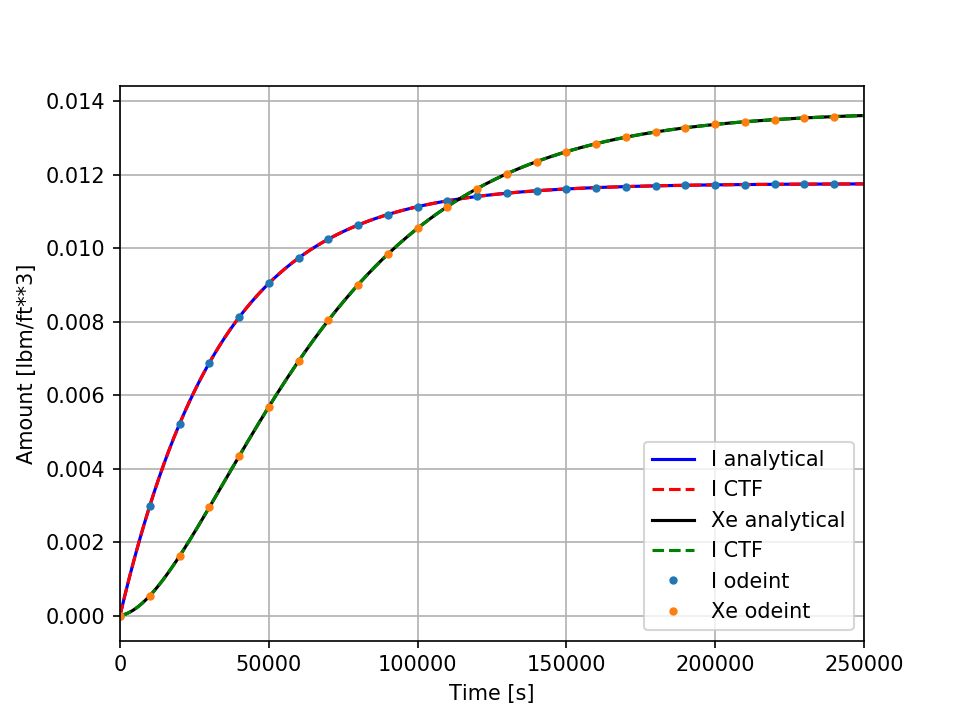
\includegraphics[width=5in]{images/XeIBuildup.png}\\
  \caption{Xe and I build up}
  \label{fig:Xe_I_buildup_source_problem}
\end{figure}

\begin{figure}[ht] 
\centering
\begin{minipage}{.5\textwidth}
  \centering
  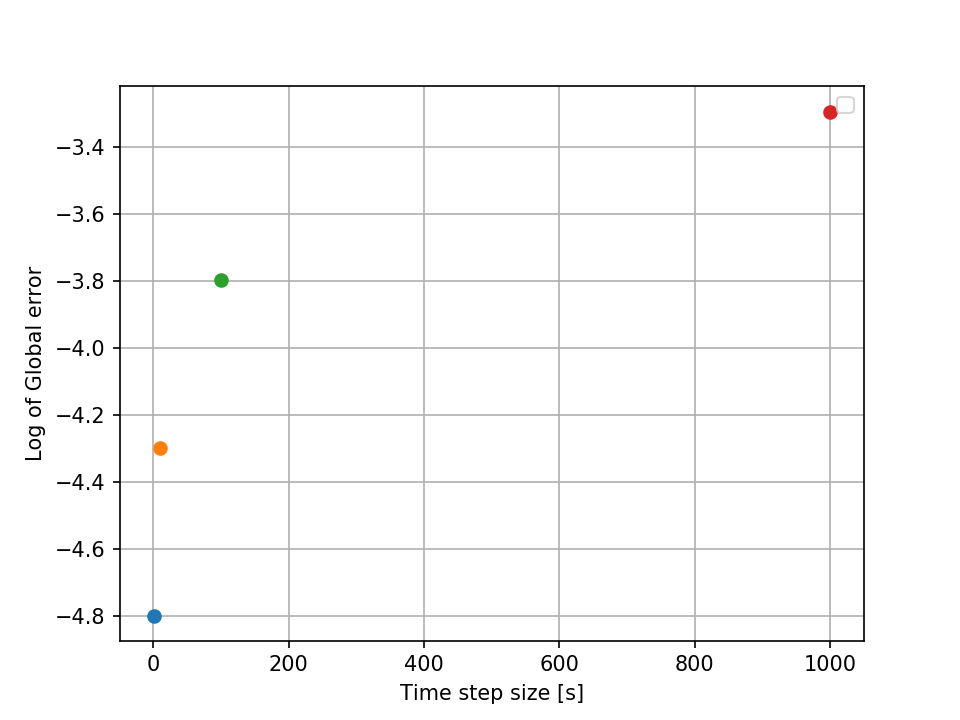
\includegraphics[width=.9\linewidth]{images/IError.png}
  \captionof{figure}{Iodine error}
  \label{fig:I_error_source_term}
\end{minipage}%
\begin{minipage}{.5\textwidth}
  \centering
  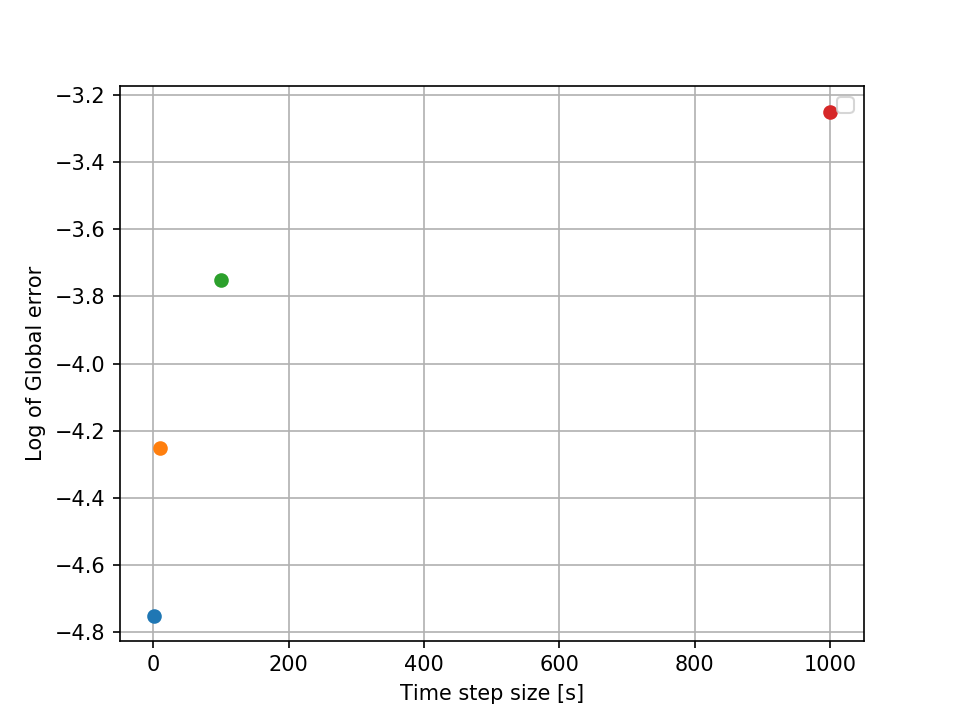
\includegraphics[width=.9\linewidth]{images/XeError.png}
  \captionof{figure}{Xenon error}
  \label{fig:Xe_error_source_term}
\end{minipage}
\end{figure}

Figure \ref{fig:Xe_I_buildup_source_problem} shows three different solutions; analytical, CTF and odeint. We have already discussed the analytical and CTF solutions, the odeint solution comes from the Python module Scipy and is a general ODE solver. All three solutions show good accordance with one another. From Figures \ref{fig:I_error_source_term} \ref{fig:Xe_error_source_term} you can see the global error decreases with decreasing time step size. 

% Single Channel Axial Step change
\subsection{Single Channel Axial Step Change}
This problem consist of a single 1 meter long channel with a varying number of axial levels. There are no source terms in the channel, only advection in the x direction. Initially the inlet concentration is set to 50 with a step change occurring for time greater then 5 seconds. A summary of the problem is shown in Equation \ref{eq:axial_step_change}.

\begin{equation}
\frac{\partial C}{\partial t} = -v_{z} \frac{\partial C}{\partial z} \quad \quad C_{o} = \begin{cases}
5 &  5 > t > 0\\
10 & 5 \geq t
\end{cases}
\label{eq:axial_step_change}
\end{equation}

Figure \ref{fig:axial_step_change} shows the concentration at the outlet of the pipe for three axial meshes. The orange line is the analytical concentration at the outlet of the pipe based on the fluid velocity. For large dx values, the tails on the left and right hand side of the orange line are indicative of numerical diffusion \cite{versteeg2007}. Decreasing the axial meshing size leads to a better approximation to the solution and reduces the error cause by numerical diffusion. 

% Lateral flow step change
\subsection{Multi-channel Lateral Flow Step Change}
Lateral flow is tested in a similar manor to the axial step change test. The only difference is that channels must be stacked next to one another to build the geometry. Instead of being able to change the number of axial levels in a single channel, we must change the number of channel in the problem itself and to change the geometry of each channel as the values of dz become smaller. 

Figure \ref{fig:latFlowResults} shows the outlet concentration. The results mimic the axial flow results, showing numerical diffusion decreases as the lateral meshing gets smaller. 

% Single channel non-constant neutron flux
\subsection{Single Channel Axial Neutron Flux}
The purpose of this problem is to test advective mass transport inside CTF with nonuniform neutron flux. This problem 
consist of a single channel with 100 levels. A neutron flux represented by Equation \ref{eq:variable_neutron_flux}.

\begin{align}
   \phi = \phi_{\theta}\sin\left(\frac{\pi z}{z_{max}}\right)
   & \label{eq:variable_neutron_flux}
\end{align}

\vspace{12.7mm} %5mm vertical space

\begin{figure}[ht] 
\centering
\begin{minipage}{.5\textwidth}
  \centering
  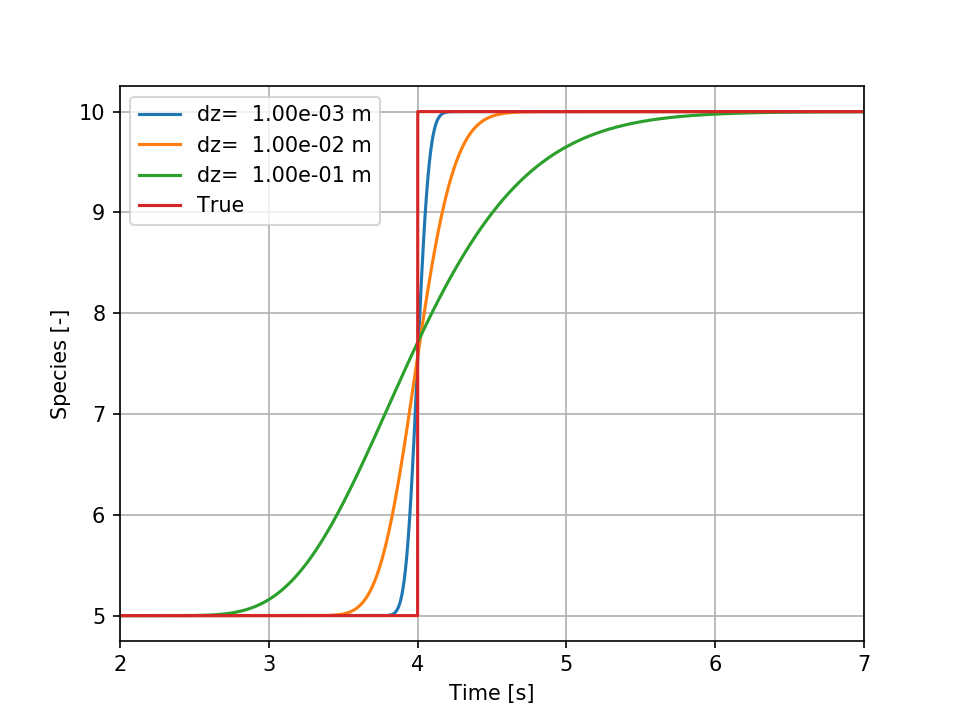
\includegraphics[width=.9\linewidth]{images/transportSpeciesLateral.png}
  \captionof{figure}{Outlet concentration as \\ a function of time for lateral flow}
  \label{fig:latFlowResults}
\end{minipage}%
\begin{minipage}{.5\textwidth}
  \centering
  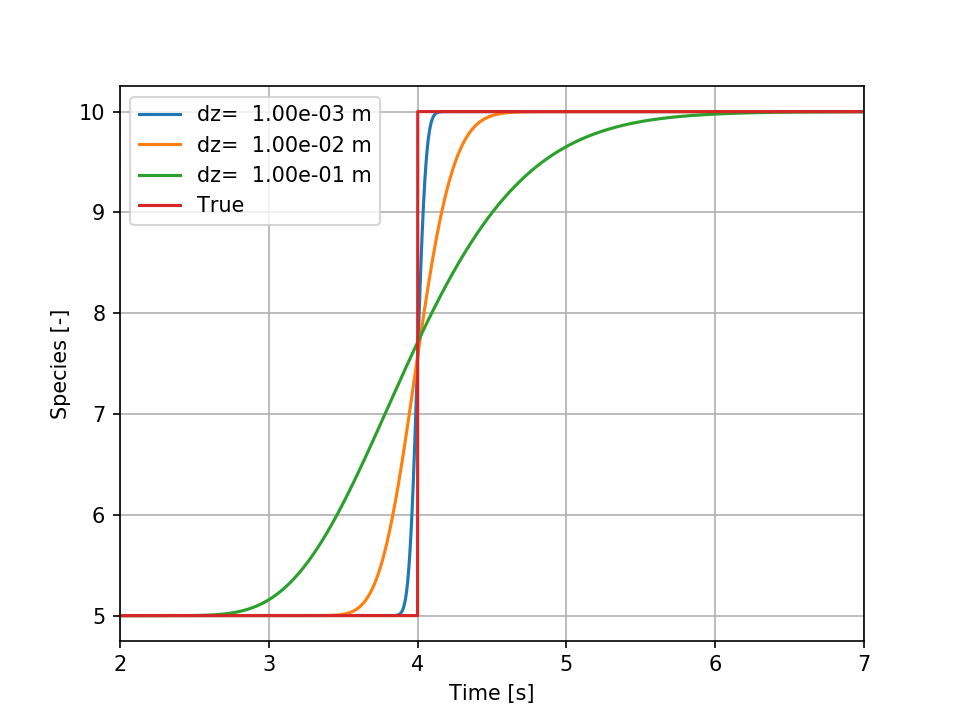
\includegraphics[width=.9\linewidth]{images/transportSpeciesConvection.png}
  \captionof{figure}{Outlet concentration as \\ a function of time for axial flow}
  \label{fig:axial_step_change}
\end{minipage}
\end{figure}

\newpage



In Equation \ref{eq:variable_neutron_flux} $\phi_{\theta}$ is the weighing factor and sets the maximum value at the 
midpoint in the problem. Z is the end point value for each axial level going up the channel and $z_{max}$ is the total 
length of the channel. A flux array is generated inside of the unit test driver and is called to set the flux at each level in 
the problem. The mean value theorem is implemented when generating this array. This is done to accurately represent 
the flux for each axial level as an average value which equals the flux over the integrated area. Equation 
\ref{eq:variable_neutron_flux_mean_value} represents the equation utilized in CTF to build the flux array. 

\begin{align}
   \phi = \left(\frac{1}{z_{2} - z_{1}}\right)\frac{\pi z \phi_{\theta}}{z_{max}}\left[\cos\left(\frac{\pi z_{1}}{z_{max}}\right) - \cos\left(\frac{\pi z_{1}}{z_{max}}\right)\right]
\label{eq:variable_neutron_flux_mean_value}
\end{align}

In Equation \ref{eq:variable_neutron_flux_mean_value} $z_{1}$ and $z_{2}$ represent the bottom and top value for the 
axial level of integration. 

For this case, we look at the transport of ${}^{135}I$ governed by Equation \ref{eq:IodineGeneralDiffEq} for steady state 1-D flow at constant velocity (v).

\begin{equation}
    \frac{d\rho_{I}}{dz} = \frac{1}{v_{z}}\bigg[\frac{M_{I}\gamma_{I}\Sigma_{f}\phi_{\theta}}{N_{A}}\sin\left(\frac{\pi z}{z_{max}}\right) - \lambda_{I}\rho_{I}\bigg]
    \label{eq:Iodine1D}
\end{equation}

The analytical solution is:

\begin{equation}
    \rho_{I}(z) = \frac{M_{I}\pi\gamma_{I}\Sigma_{f}\phi_{\theta}}{z_{max} v Na  A}e^{-\frac{\lambda_{I}z}{v}} - \frac{M_{I}\gamma_{I}\Sigma_{f}\phi_{\theta}}{ v Na  A}\bigg[ \frac{\pi}{z_{max}}\cos{\left(\frac{\pi z}{z_{max}}\right)}-\frac{\lambda_{I}}{v}\sin{\left(\frac{\pi z}{z_{max}}\right)}\bigg]
\end{equation}

\begin{equation*}
    A = \frac{\lambda_{I}^{2}}{v^{2}} + \frac{\pi^{2}}{z_{max}^{2}}
\end{equation*}

Figure \ref{fig:iodine_flux_solution} shows the analytical vs. CTF solution for a system of 100 axial levels. Figure \ref{fig:iodine_flux_error} gives the log of the global error vs. the dz step size. 

\begin{figure}[ht] 
\centering
\begin{minipage}{.5\textwidth}
  \centering
  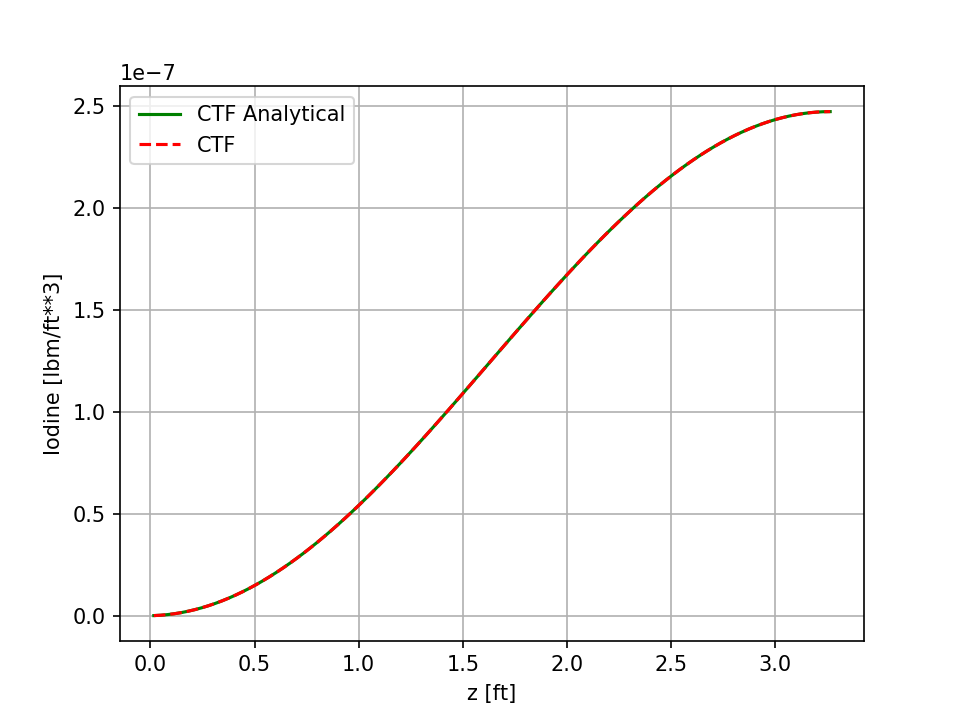
\includegraphics[width=.9\linewidth]{images/transportedSpeciesAxialNonuniform.png}
  \captionof{figure}{Iodine solution}
  \label{fig:iodine_flux_solution}
\end{minipage}%
\begin{minipage}{.5\textwidth}
  \centering
  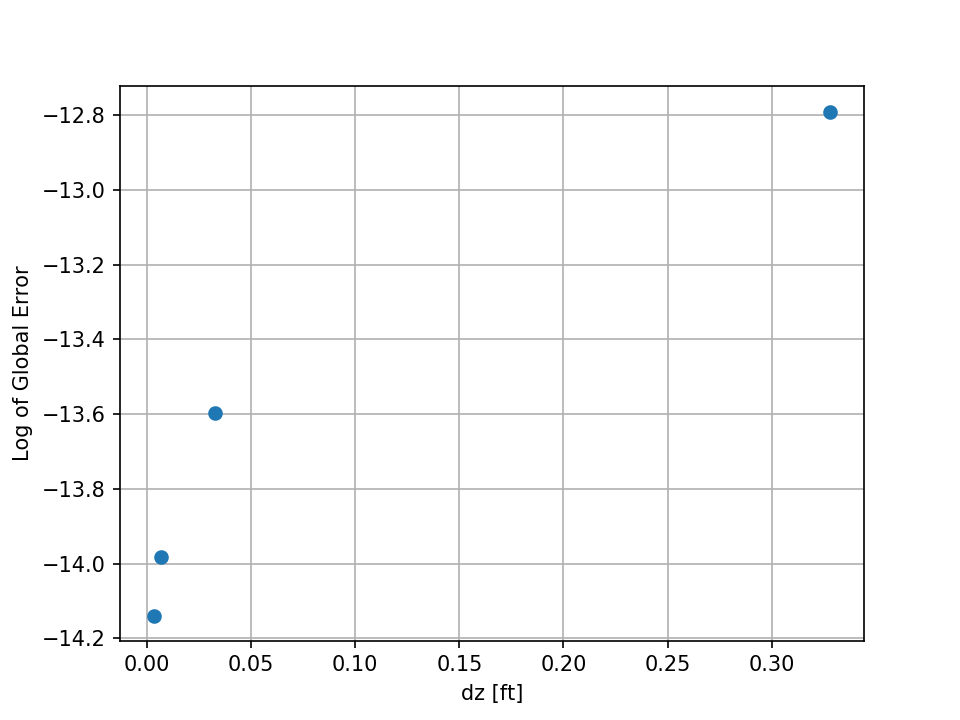
\includegraphics[width=.9\linewidth]{images/transportedSpeciesAxialNonuniformError.png}
  \captionof{figure}{Global error}
  \label{fig:iodine_flux_error}
\end{minipage}
\end{figure}

\newpage

% multiphase species transport
\section{Multi-phase Species Transport}\label{sec:gas_transport}

\subsection{Bubble Growth}
Bubble growth is governed by changes in temperature, pressure and mass. Equation \ref{eq:ideal_gas_law_volume} shows the relation between volume, temperature, pressure and mass. 

\begin{equation}
	V = \frac{nRT}{P}
	\label{eq:ideal_gas_law_volume}
\end{equation}

Volume is directly proportional to moles (n) and temperature (T) and inversely proportional to pressure (P). This means that increasing moles or temperature will cause a direct increase in volume. Increasing the pressure will decrease the bubble volume, leading to an overall decrease in interfacial area. The following cases test this relationship to ensure an accurate representation of bubble dynamics. 

In each of the following test a single 10 level channel is used to determine each variables impact on interfacial area and bubble diameter. The specified variable linearly increases as the species flow up the channel. At the end of the channel, the interfacial area and bubble diameter will be accessed to determine if it increased or decreased. An analytical solution will not be addressed, only the general trend. 

% Temperature effect
\subsubsection{Temperature}
Temperature linearly increases up the channel, bubble diameter and interfacial area are shown in Figures \ref{fig:temp_increase_bubDia} and \ref{fig:temp_increase_intArea}. Figures \ref{fig:temp_decrease_bubDia} and \ref{fig:temp_decrease_intArea} demonstrate the effect of a temperature decrease.

%Pressure effect
\subsubsection{Pressure}
Figures \ref{fig:press_increase_bubDia} and \ref{fig:press_increase_intArea} show bubble diameter and interfacial area under a pressure increase. Figures \ref{fig:press_decrease_bubDia} and \ref{fig:press_decrease_intArea} show a the same variables under and pressure decrease.

\subsubsection{Mass}
Testing masses effect was a little different than temperature and pressure. In the previous two cases mass transfer into or out of the bubble was stopped by setting the mass transfer coefficient (k) to zero. K is set to a small positive value to simulate mass leaving the bubbles. Mass entering the bubbles is achieved by switching the sign of k. A small k value is need to ensure that equilibrium isn't reached between the liquid and gas phase. This will cause bubble diameter and interfacial area to continuously increase or decrease up the channel. Figures \ref{fig:mass_increase_bubDia} through \ref{fig:mass_decrease_intArea} exhibit mass transfer from the bubbles.

\subsection{Interfacial Area Source}
Phase migration is testing in a single channel with two chemical species helium and xenon. At the bottom of the channel helium bubbles at reference diameter $(D_{ref})$ are inject along with xenon dissolved in the liquid phase. As the mixture travels up the channel xenon migrates into the helium bubbles with both streams exiting at the top of the channel. Xenon migration is governed by Equation \ref{eq:liq_side_coupling} where the value for $k$ is taken from \cite{houtzeel1967}. Helium is not allowed to dissolve in the salt by making its mass transfer coefficient zero. Table \ref{tab:intArea_test_parameters} summarizes important parameters utilized in the test.  

\FloatBarrier
\newpage

\begin{figure}[p] 
\centering
\begin{minipage}{.5\textwidth}
  \centering
  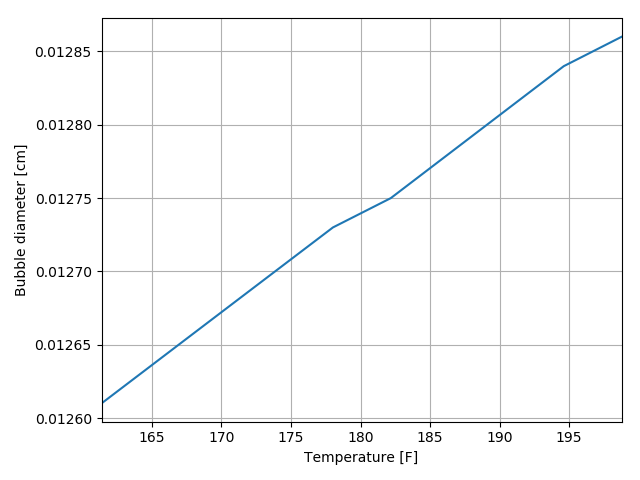
\includegraphics[width=.9\linewidth]{images/BubbleDiaTemperatureIncrease.png}
  \captionof{figure}{effect of temperature increase \\ on bubble diameter}
  \label{fig:temp_increase_bubDia}
\end{minipage}%
\begin{minipage}{.5\textwidth}
  \centering
  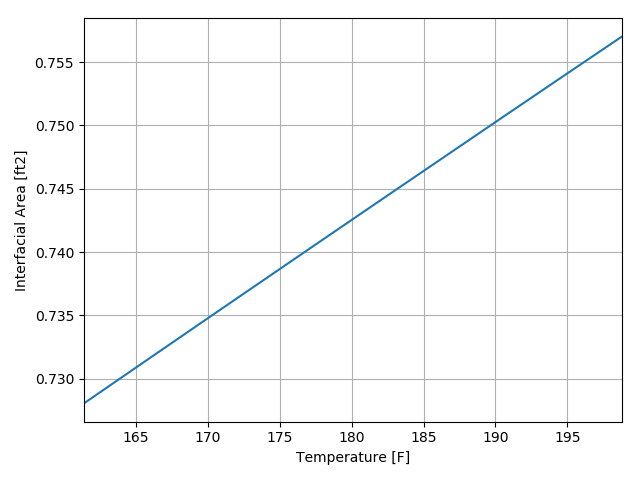
\includegraphics[width=.9\linewidth]{images/IntAreaTemperatureIncrease.png}
  \captionof{figure}{Effect of temperature increase \\ on interfacial area}
  \label{fig:temp_increase_intArea}
\end{minipage}
\end{figure}

\begin{figure}[p] 
\centering
\begin{minipage}{.5\textwidth}
  \centering
  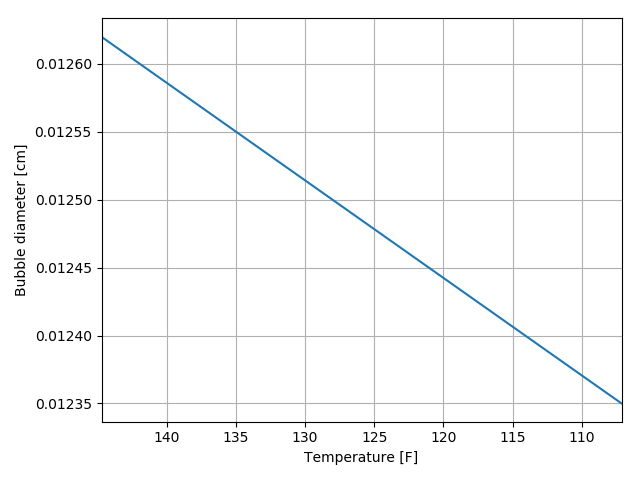
\includegraphics[width=.9\linewidth]{images/BubbleDiaTemperatureDecrease.png}
  \captionof{figure}{Effect of temperature \\ decrease  on bubble diameter}
  \label{fig:temp_decrease_bubDia}
\end{minipage}%
\begin{minipage}{.5\textwidth}
  \centering
  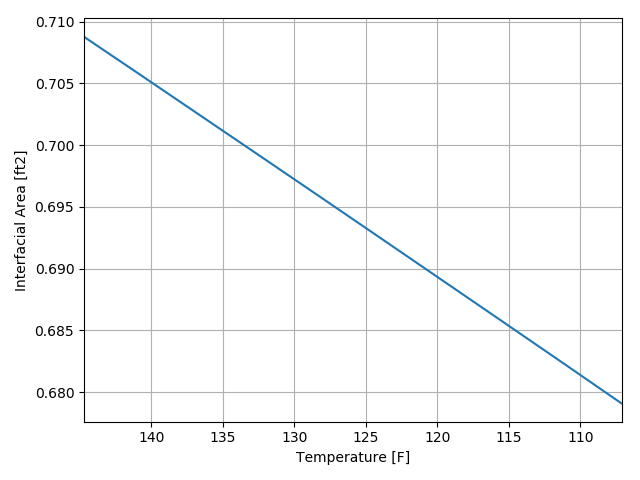
\includegraphics[width=.9\linewidth]{images/IntAreaTemperatureDecrease.png}
  \captionof{figure}{Effect of temperature \\ decrease on interfacial area}
  \label{fig:temp_decrease_intArea}
\end{minipage}
\end{figure}

\FloatBarrier
\newpage
\FloatBarrier

\begin{figure}[p] 
\centering
\begin{minipage}{.5\textwidth}
  \centering
  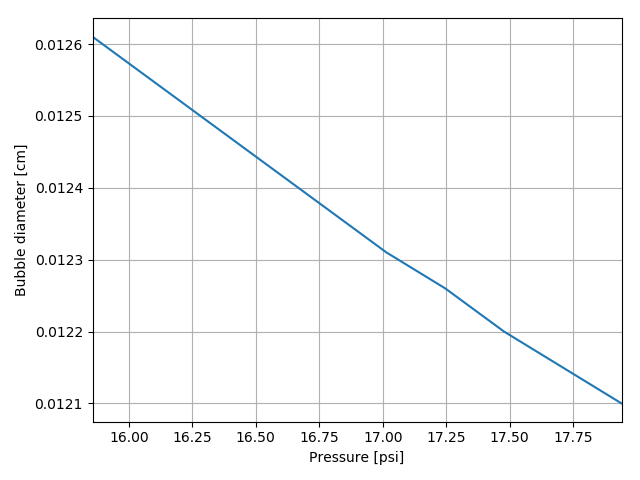
\includegraphics[width=.9\linewidth]{images/BubbleDiaPressureIncrease.png}
  \captionof{figure}{Effect of pressure increase \\ on bubble diameter}
  \label{fig:press_increase_bubDia}
\end{minipage}%
\begin{minipage}{.5\textwidth}
  \centering
  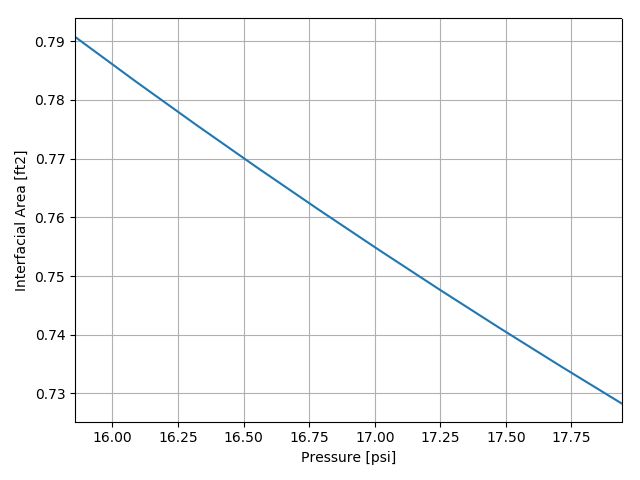
\includegraphics[width=.9\linewidth]{images/IntAreaPressureIncrease.png}
  \captionof{figure}{Effect of pressure increase \\ on interfacial area}
  \label{fig:press_increase_intArea}
\end{minipage}
\end{figure}

\begin{figure}[p] 
\centering
\begin{minipage}{.5\textwidth}
  \centering
  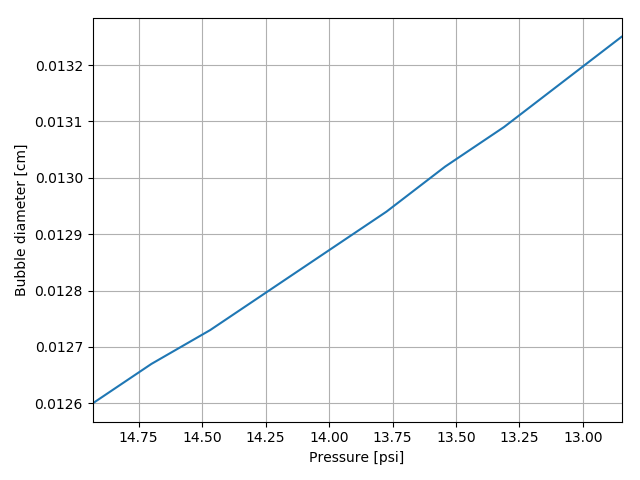
\includegraphics[width=.9\linewidth]{images/BubbleDiaPressureDecrease.png}
  \captionof{figure}{Effect of pressure decrease \\ on bubble diameter}
  \label{fig:press_decrease_bubDia}
\end{minipage}%
\begin{minipage}{.5\textwidth}
  \centering
  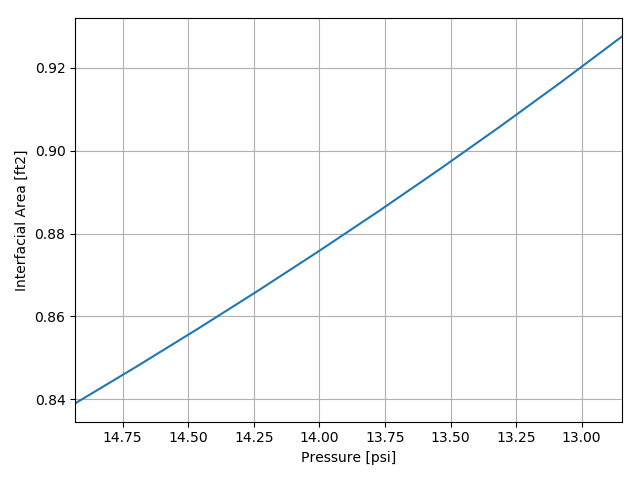
\includegraphics[width=.9\linewidth]{images/IntAreaPressureDecrease.png}
  \captionof{figure}{Effect of pressure decrease \\ on interfacial area}
  \label{fig:press_decrease_intArea}
\end{minipage}
\end{figure}

\FloatBarrier
\newpage
\FloatBarrier



\begin{figure}[p] 
\centering
\begin{minipage}{.5\textwidth}
  \centering
  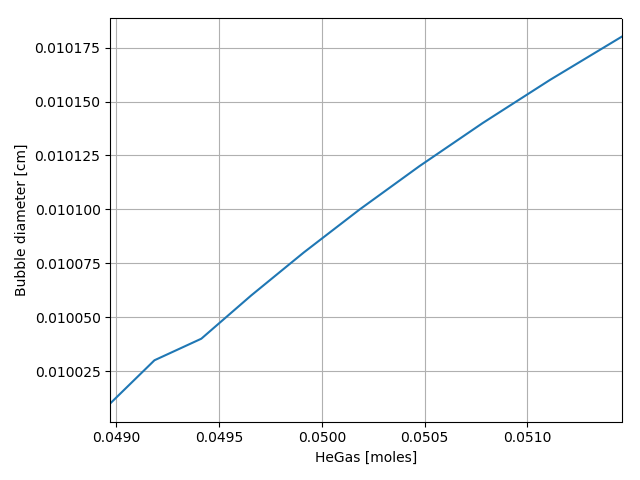
\includegraphics[width=.9\linewidth]{images/BubbleDiaMassIncrease.png}
  \captionof{figure}{Effect of mass increase \\ on bubble diameter}
  \label{fig:mass_increase_bubDia}
\end{minipage}%
\begin{minipage}{.5\textwidth}
  \centering
  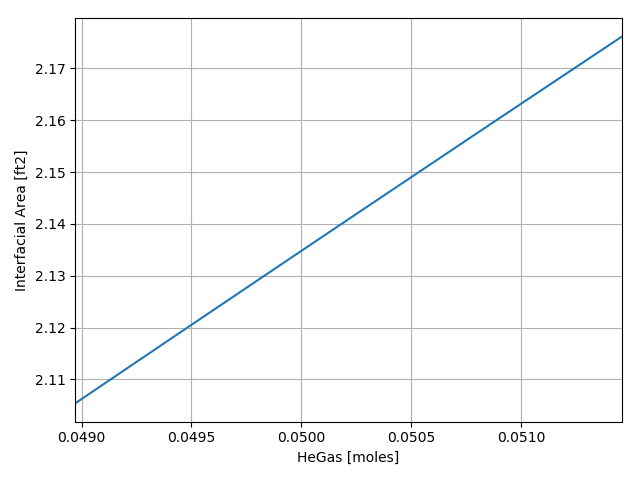
\includegraphics[width=.9\linewidth]{images/IntAreaMassIncrease.png}
  \captionof{figure}{Effect of mass increase \\ on interfacial area}
  \label{fig:mass_increase_intArea}
\end{minipage}
\end{figure}

\begin{figure}[p] 
\centering
\begin{minipage}{.5\textwidth}
  \centering
  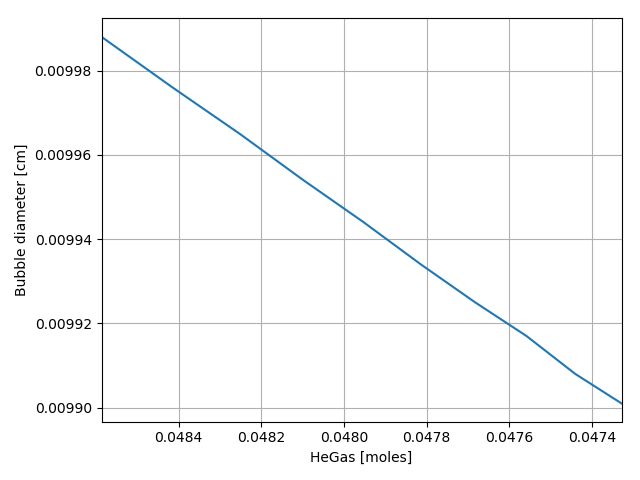
\includegraphics[width=.9\linewidth]{images/BubbleDiaMassDecrease.png}
  \captionof{figure}{Effect of mass decrease \\ on bubble diameter}
  \label{fig:mass_decrease_bubDia}
\end{minipage}%
\begin{minipage}{.5\textwidth}
  \centering
  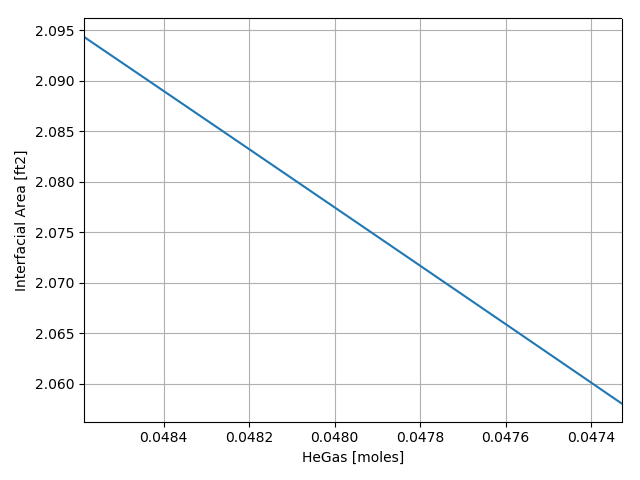
\includegraphics[width=.9\linewidth]{images/IntAreaMassDecrease.png}
  \captionof{figure}{Effect of mass decrease \\ on interfacial area}
  \label{fig:mass_decrease_intArea}
\end{minipage}
\end{figure}

\FloatBarrier
\newpage
\FloatBarrier



\begin{table}[htbp!]
   \caption{\label{tab:intArea_test_parameters} Problem parameters}
   \centering
   \begin{tabular}{lll}
   \hline
   \textbf{Parameter} & \textbf{Value} & \textbf{Unit} \\
   \hline 
   $k_{Xe}$ & 2.0 \cite{houtzeel1967} & ft/hr\\ [1ex]
   $k_{He}$ & 0.0 & ft/hr \\ [1ex]
   $H_{Xe}$ & 2.75E-9 \cite{houtzeel1967} & mole/cm${}^{3}$/atm \\ [1ex]
   $D_{ref}$ & 0.0127 \cite{engel1971} & cm \\ [1ex]
   He injection rate & 2.0E-6 & moles/s \\ [1ex]
   \hline
   \end{tabular}
\end{table}

The set of equations that govern the problem are a set of coupled nonlinear first order ordinary differential equations. Nonlinearality comes from the fact that interfacial area changes as a function of mass transfer into the bubbles. Equations \ref{eq:intArea_test_xeGass} through \ref{eq:intArea_test_area} are solved using scipys odeint package in Python. 

\begin{equation}
    \frac{d\rho_{Xe}^{g}}{dz} = \frac{1}{v_{z}}\bigg[\frac{kA}{V}(\rho_{Xe}^{*} - \frac{\rho_{Xe}^{l}}{1-\alpha}) \bigg]
    \label{eq:intArea_test_xeGass}
\end{equation}

\begin{equation}
    \frac{d\rho_{Xe}^{l}}{dz} = \frac{1}{v_{z}}\bigg[\frac{kA}{V}(\frac{\rho_{Xe}^{l}}{1-\alpha} - \rho_{Xe}^{*}) \bigg]
\end{equation}

\begin{equation}
    n_{bubble} = \frac{n_{Xe} + n_{He}}{\text{\# of Bubbles}}
\end{equation}

\begin{equation}
    A_{bubble} = \pi^{1/3}\bigg(\frac{6nRT}{P}\bigg)^{2/3}
\end{equation}

\begin{equation}
    A = A_{bubble} * (\text{\# of bubbles})
    \label{eq:intArea_test_area}
\end{equation}

Figures \ref{fig:IntArea_source_xe_gas_sol} and \ref{fig:IntArea_source_xe_liq_sol} show the ODE solutions, with their respective global errors in Figures \ref{fig:IntArea_source_xe_gas_error} and \ref{fig:IntArea_source_xe_liq_error}. Both CTF solutions match their gold solutions quite well. Global error for both solutions decreases by increasing the number of axial levels thus decreasing the axial step size.  


\FloatBarrier
\newpage

\begin{figure}[p] 
\centering
\begin{minipage}{.5\textwidth}
  \centering
  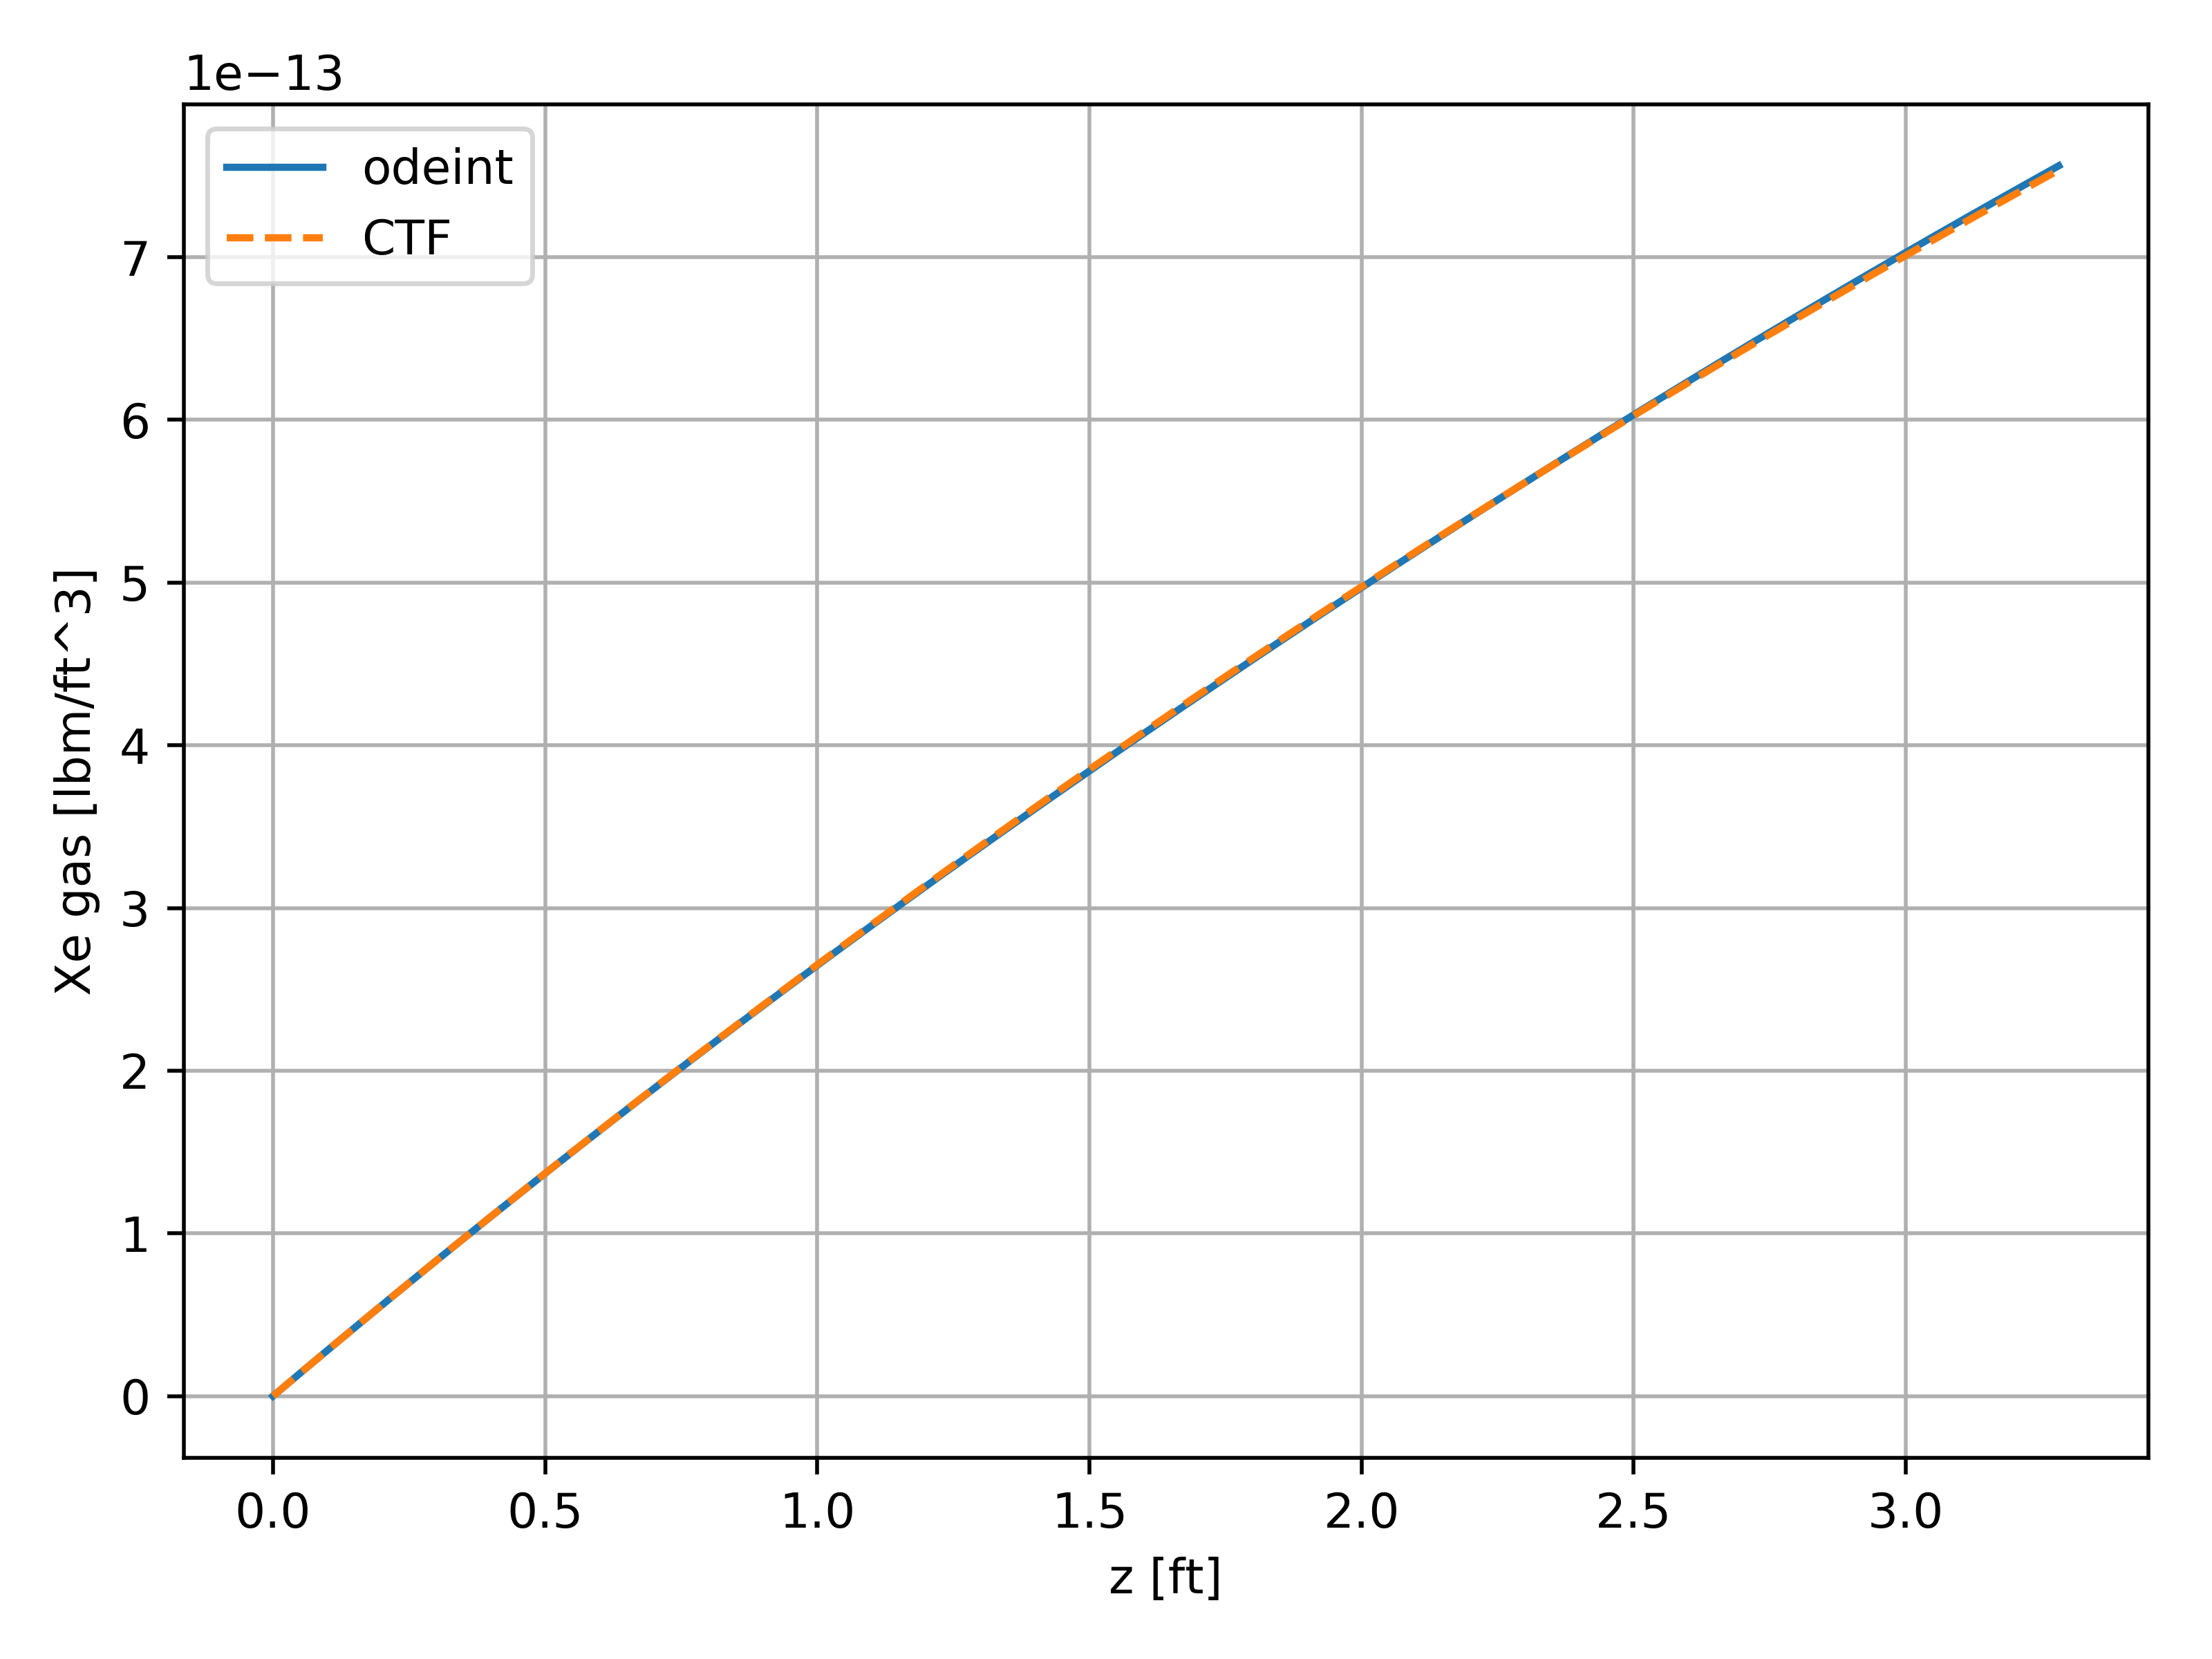
\includegraphics[width=.9\linewidth]{images/transportSpeciesIntAreaXeGas.png}
  \captionof{figure}{Xenon gas solution}
  \label{fig:IntArea_source_xe_gas_sol}
\end{minipage}%
\begin{minipage}{.5\textwidth}
  \centering
  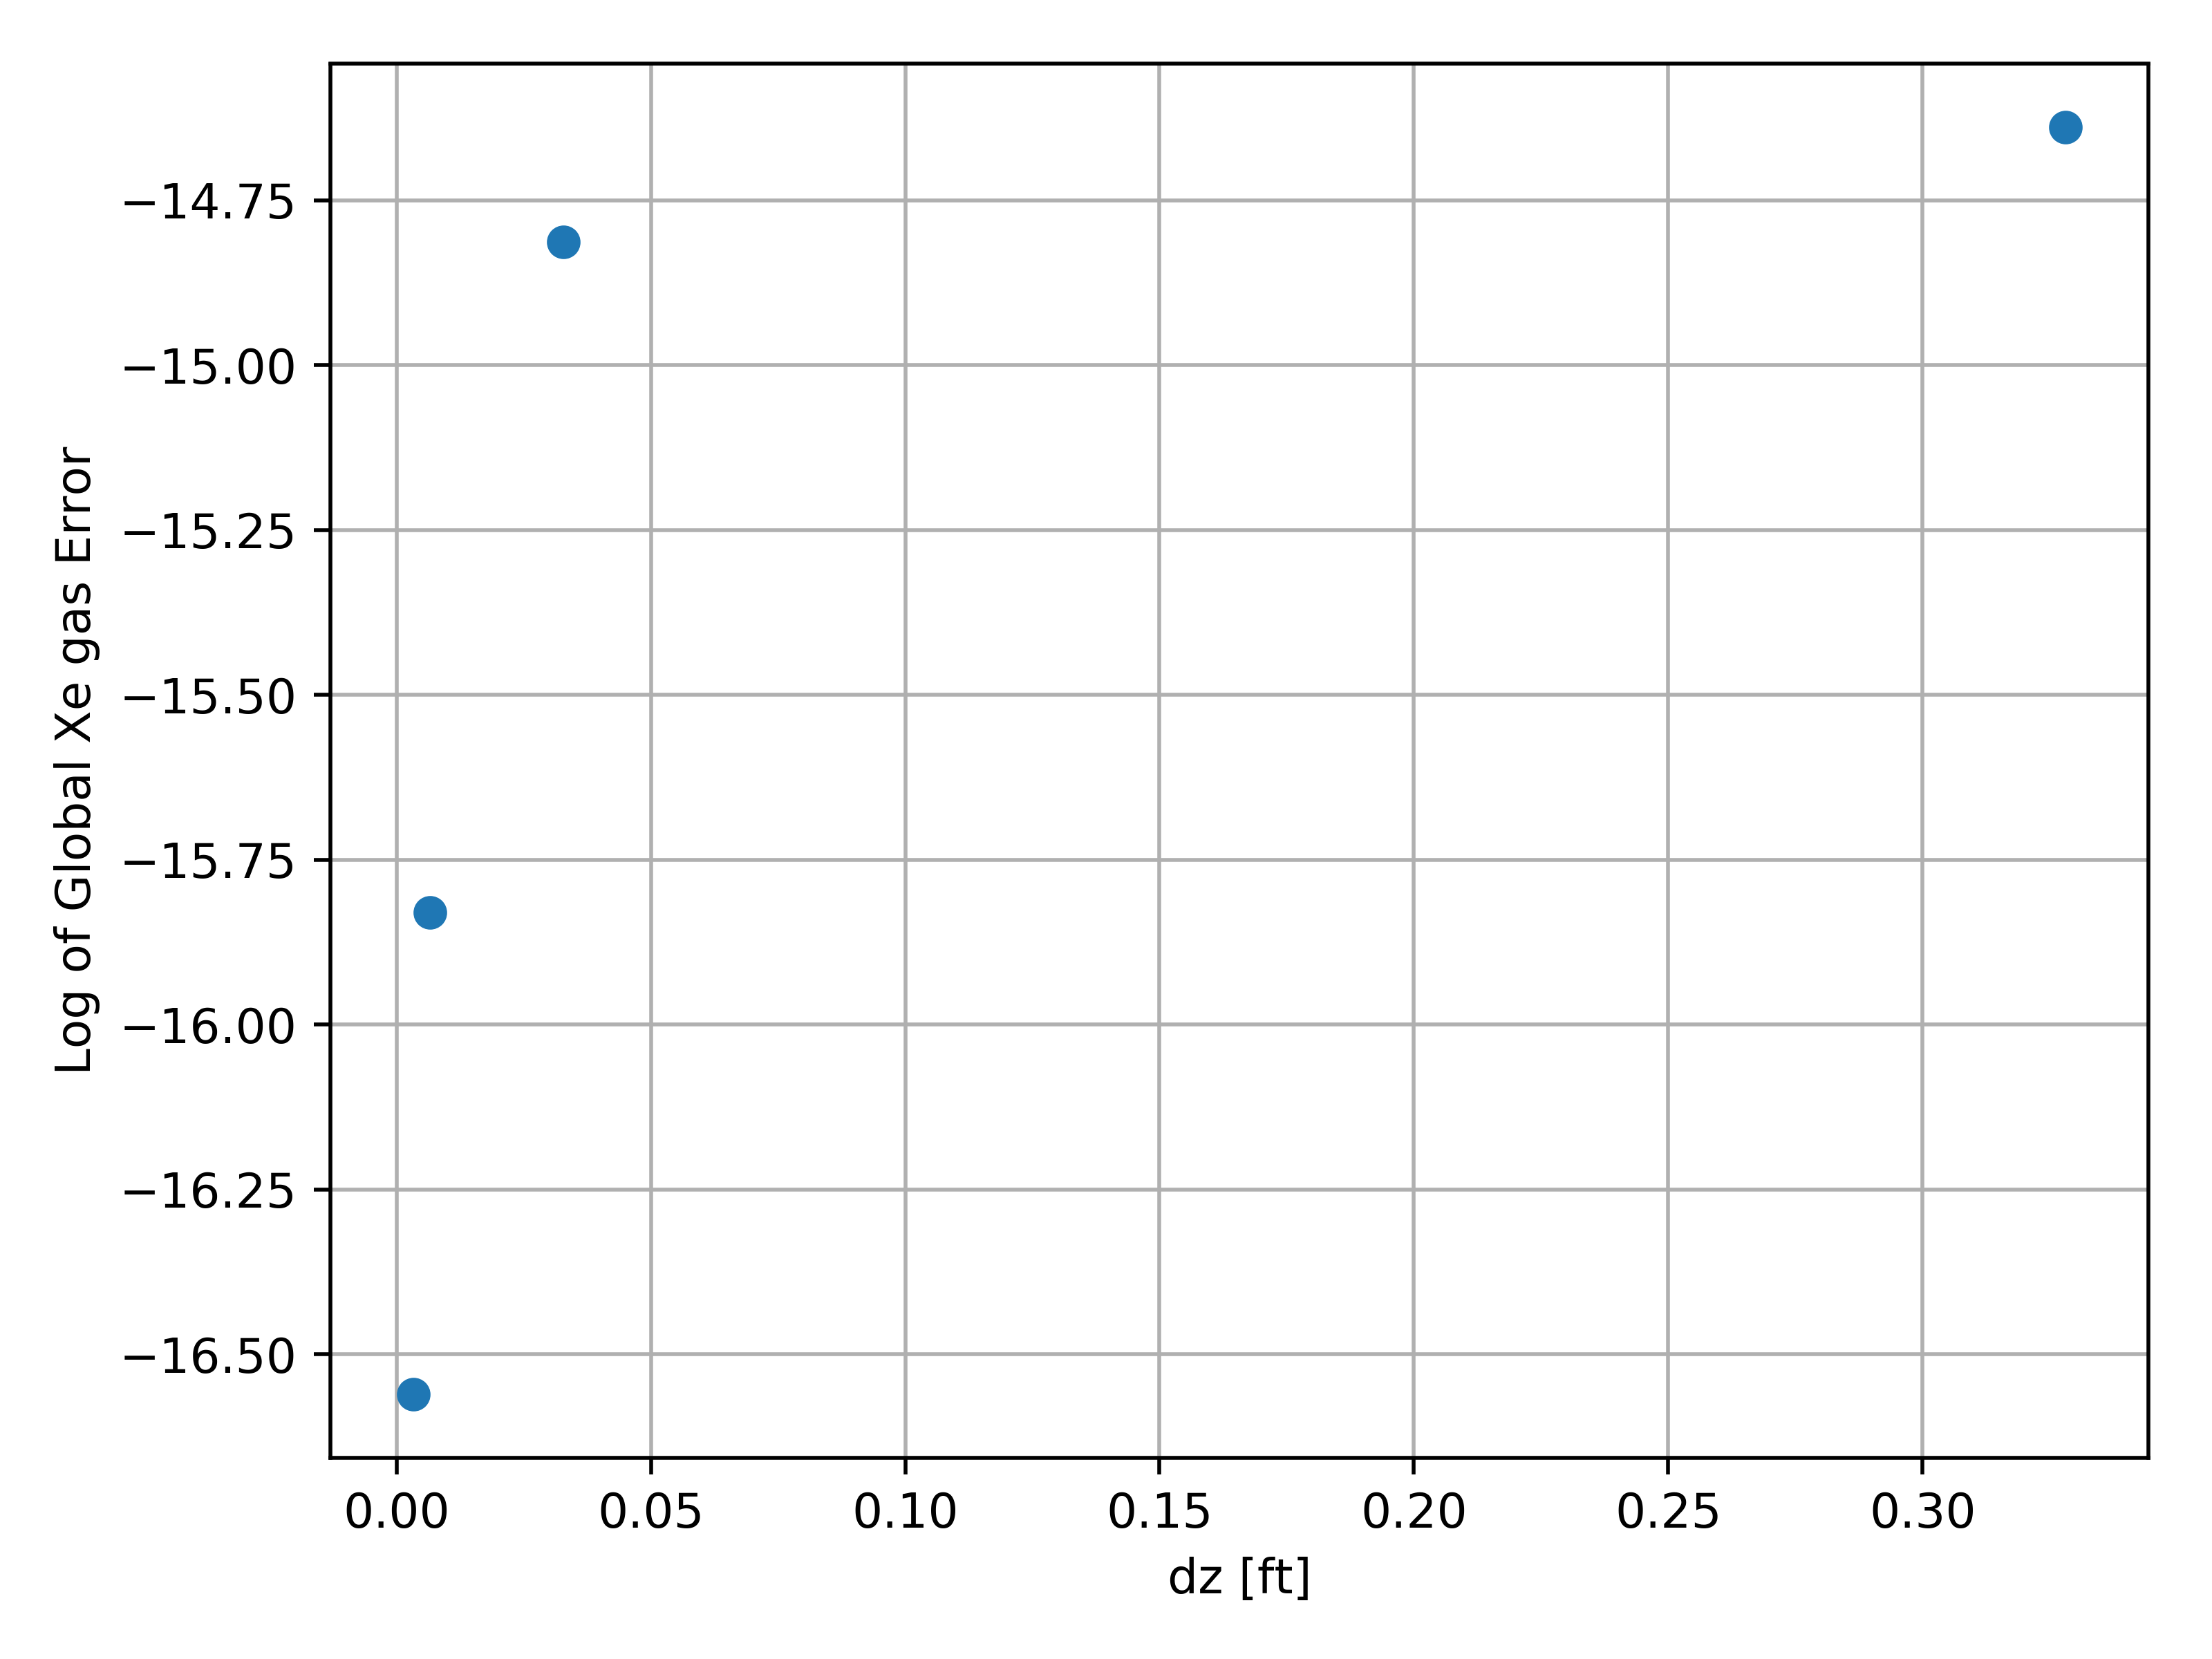
\includegraphics[width=.9\linewidth]{images/transportedSpeciesIntAreaXeGasError.png}
  \captionof{figure}{Xenon gas error vs mesh size}
  \label{fig:IntArea_source_xe_gas_error}
\end{minipage}
\end{figure}

\begin{figure}[p] 
\centering
\begin{minipage}{.5\textwidth}
  \centering
  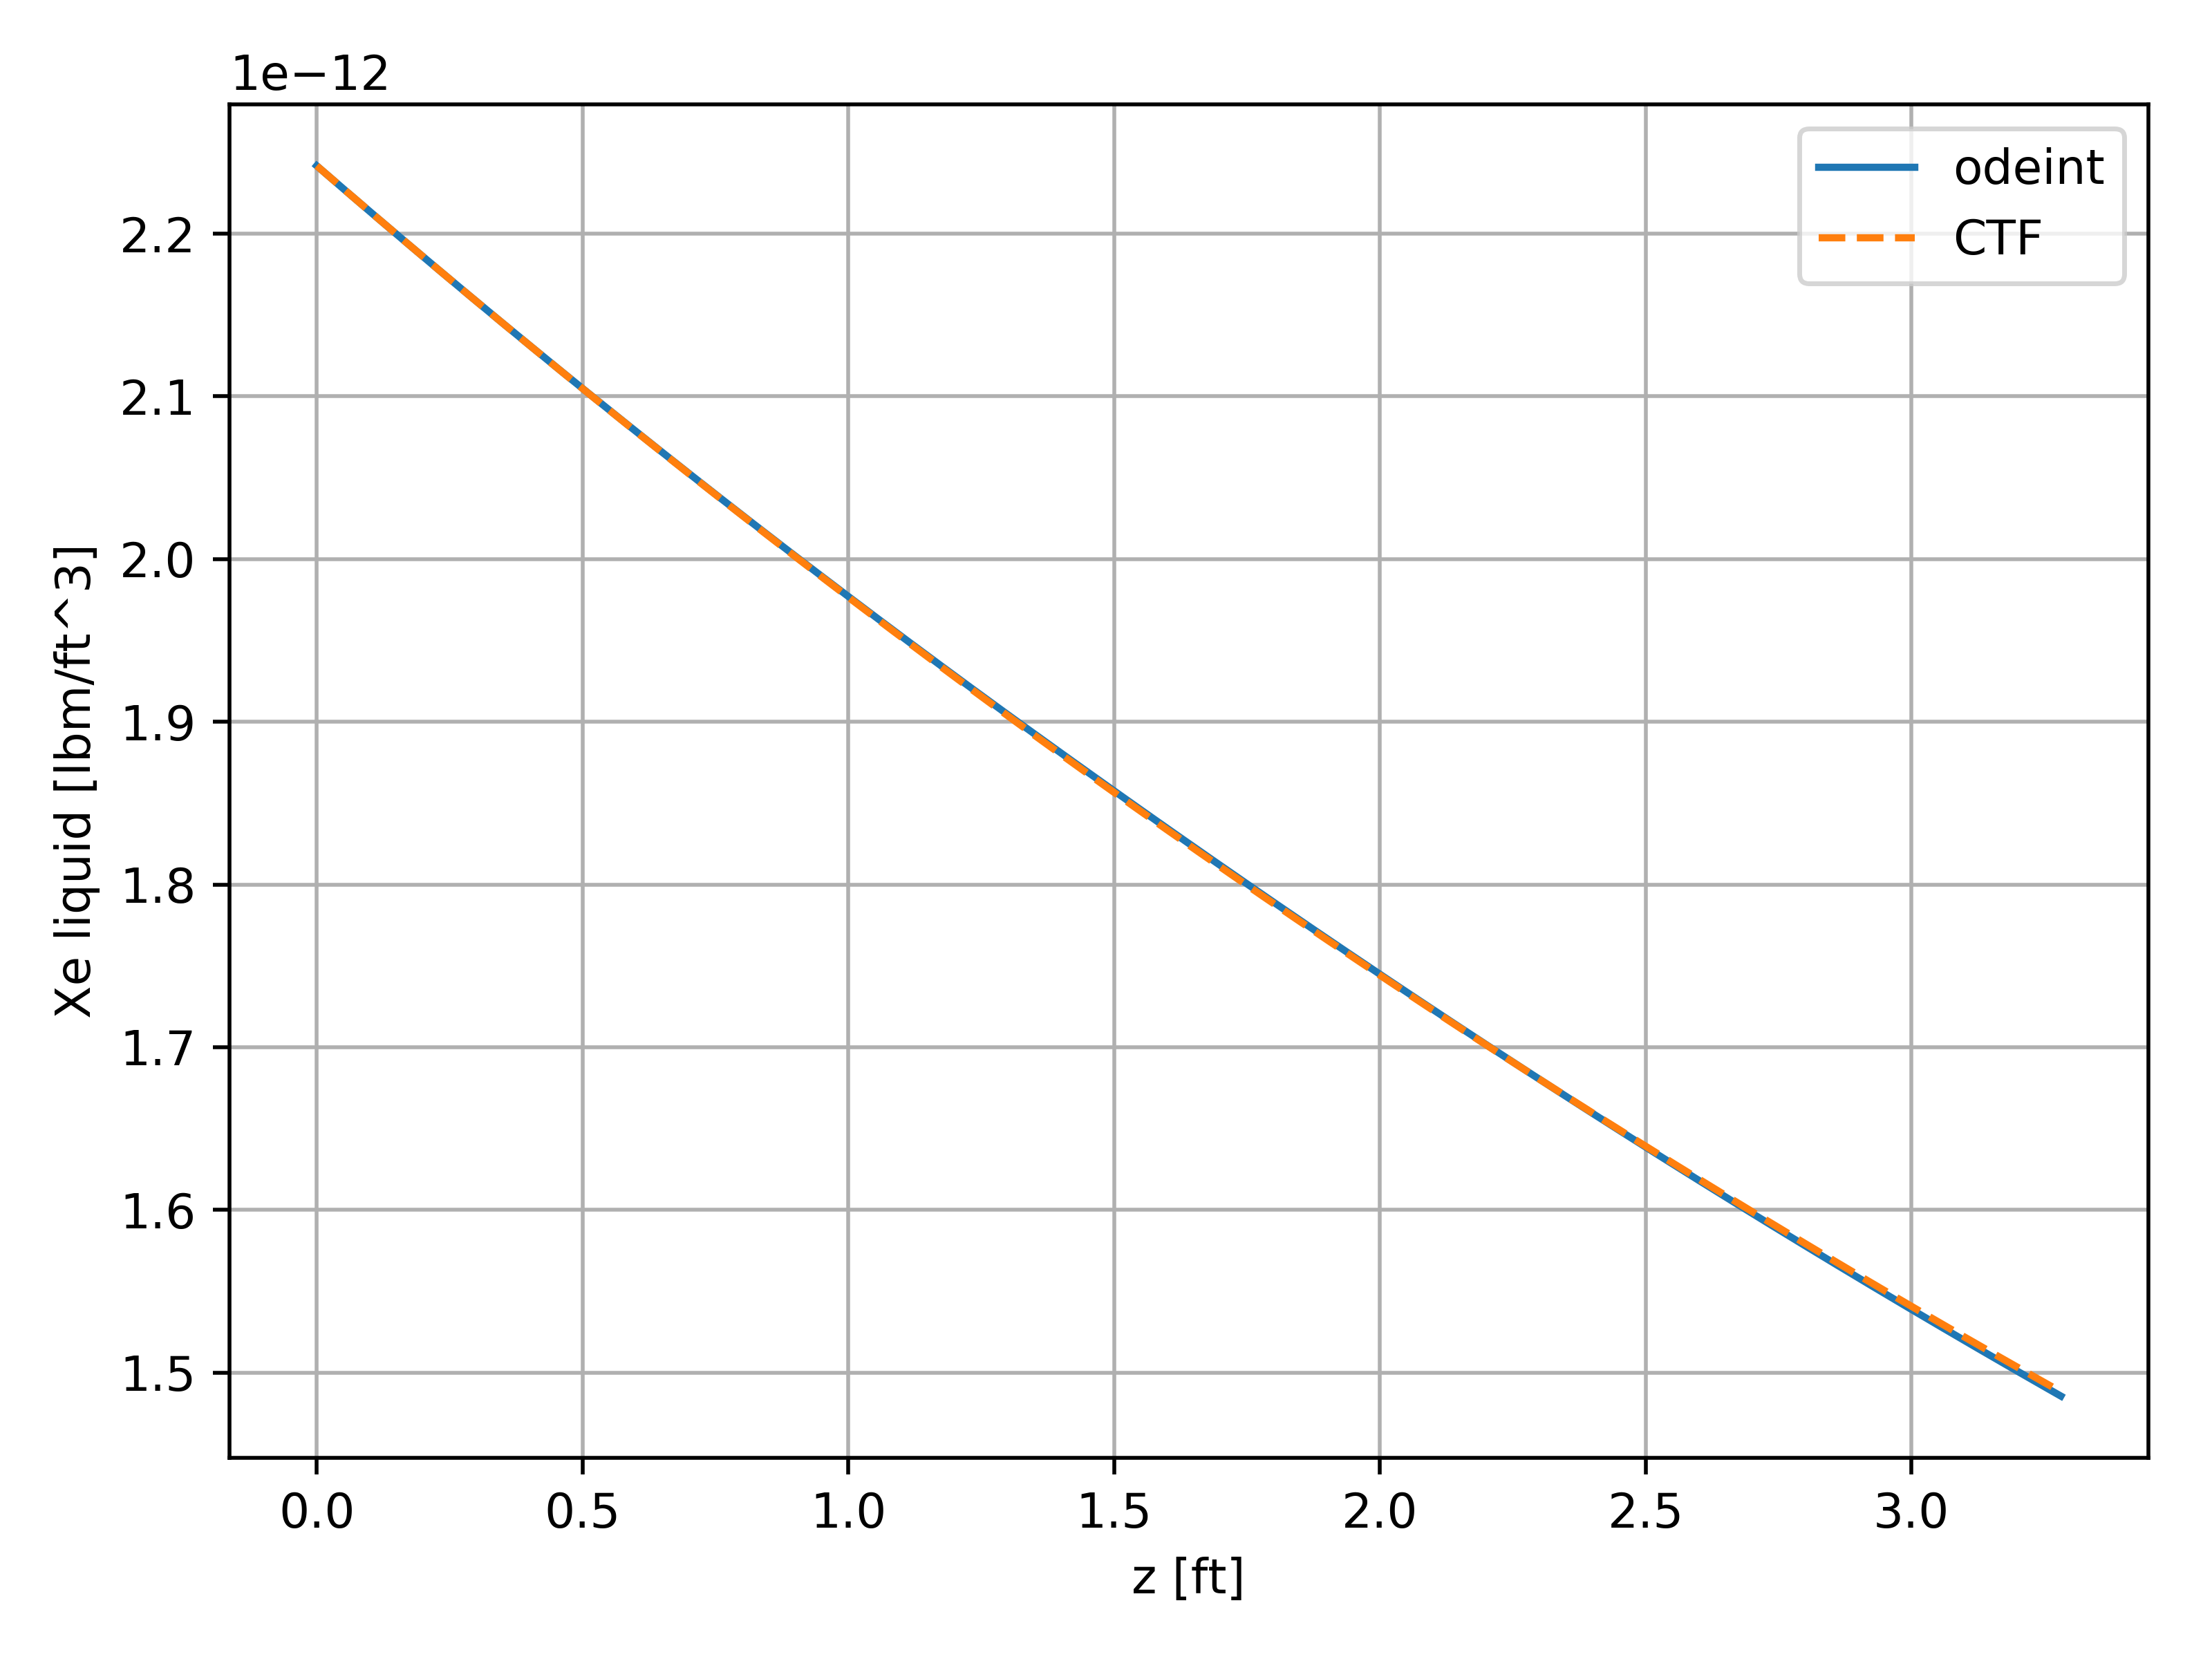
\includegraphics[width=.9\linewidth]{images/transportSpeciesIntAreaXeLiq.png}
  \captionof{figure}{Xenon liquid solution}
  \label{fig:IntArea_source_xe_liq_sol}
\end{minipage}%
\begin{minipage}{.5\textwidth}
  \centering
  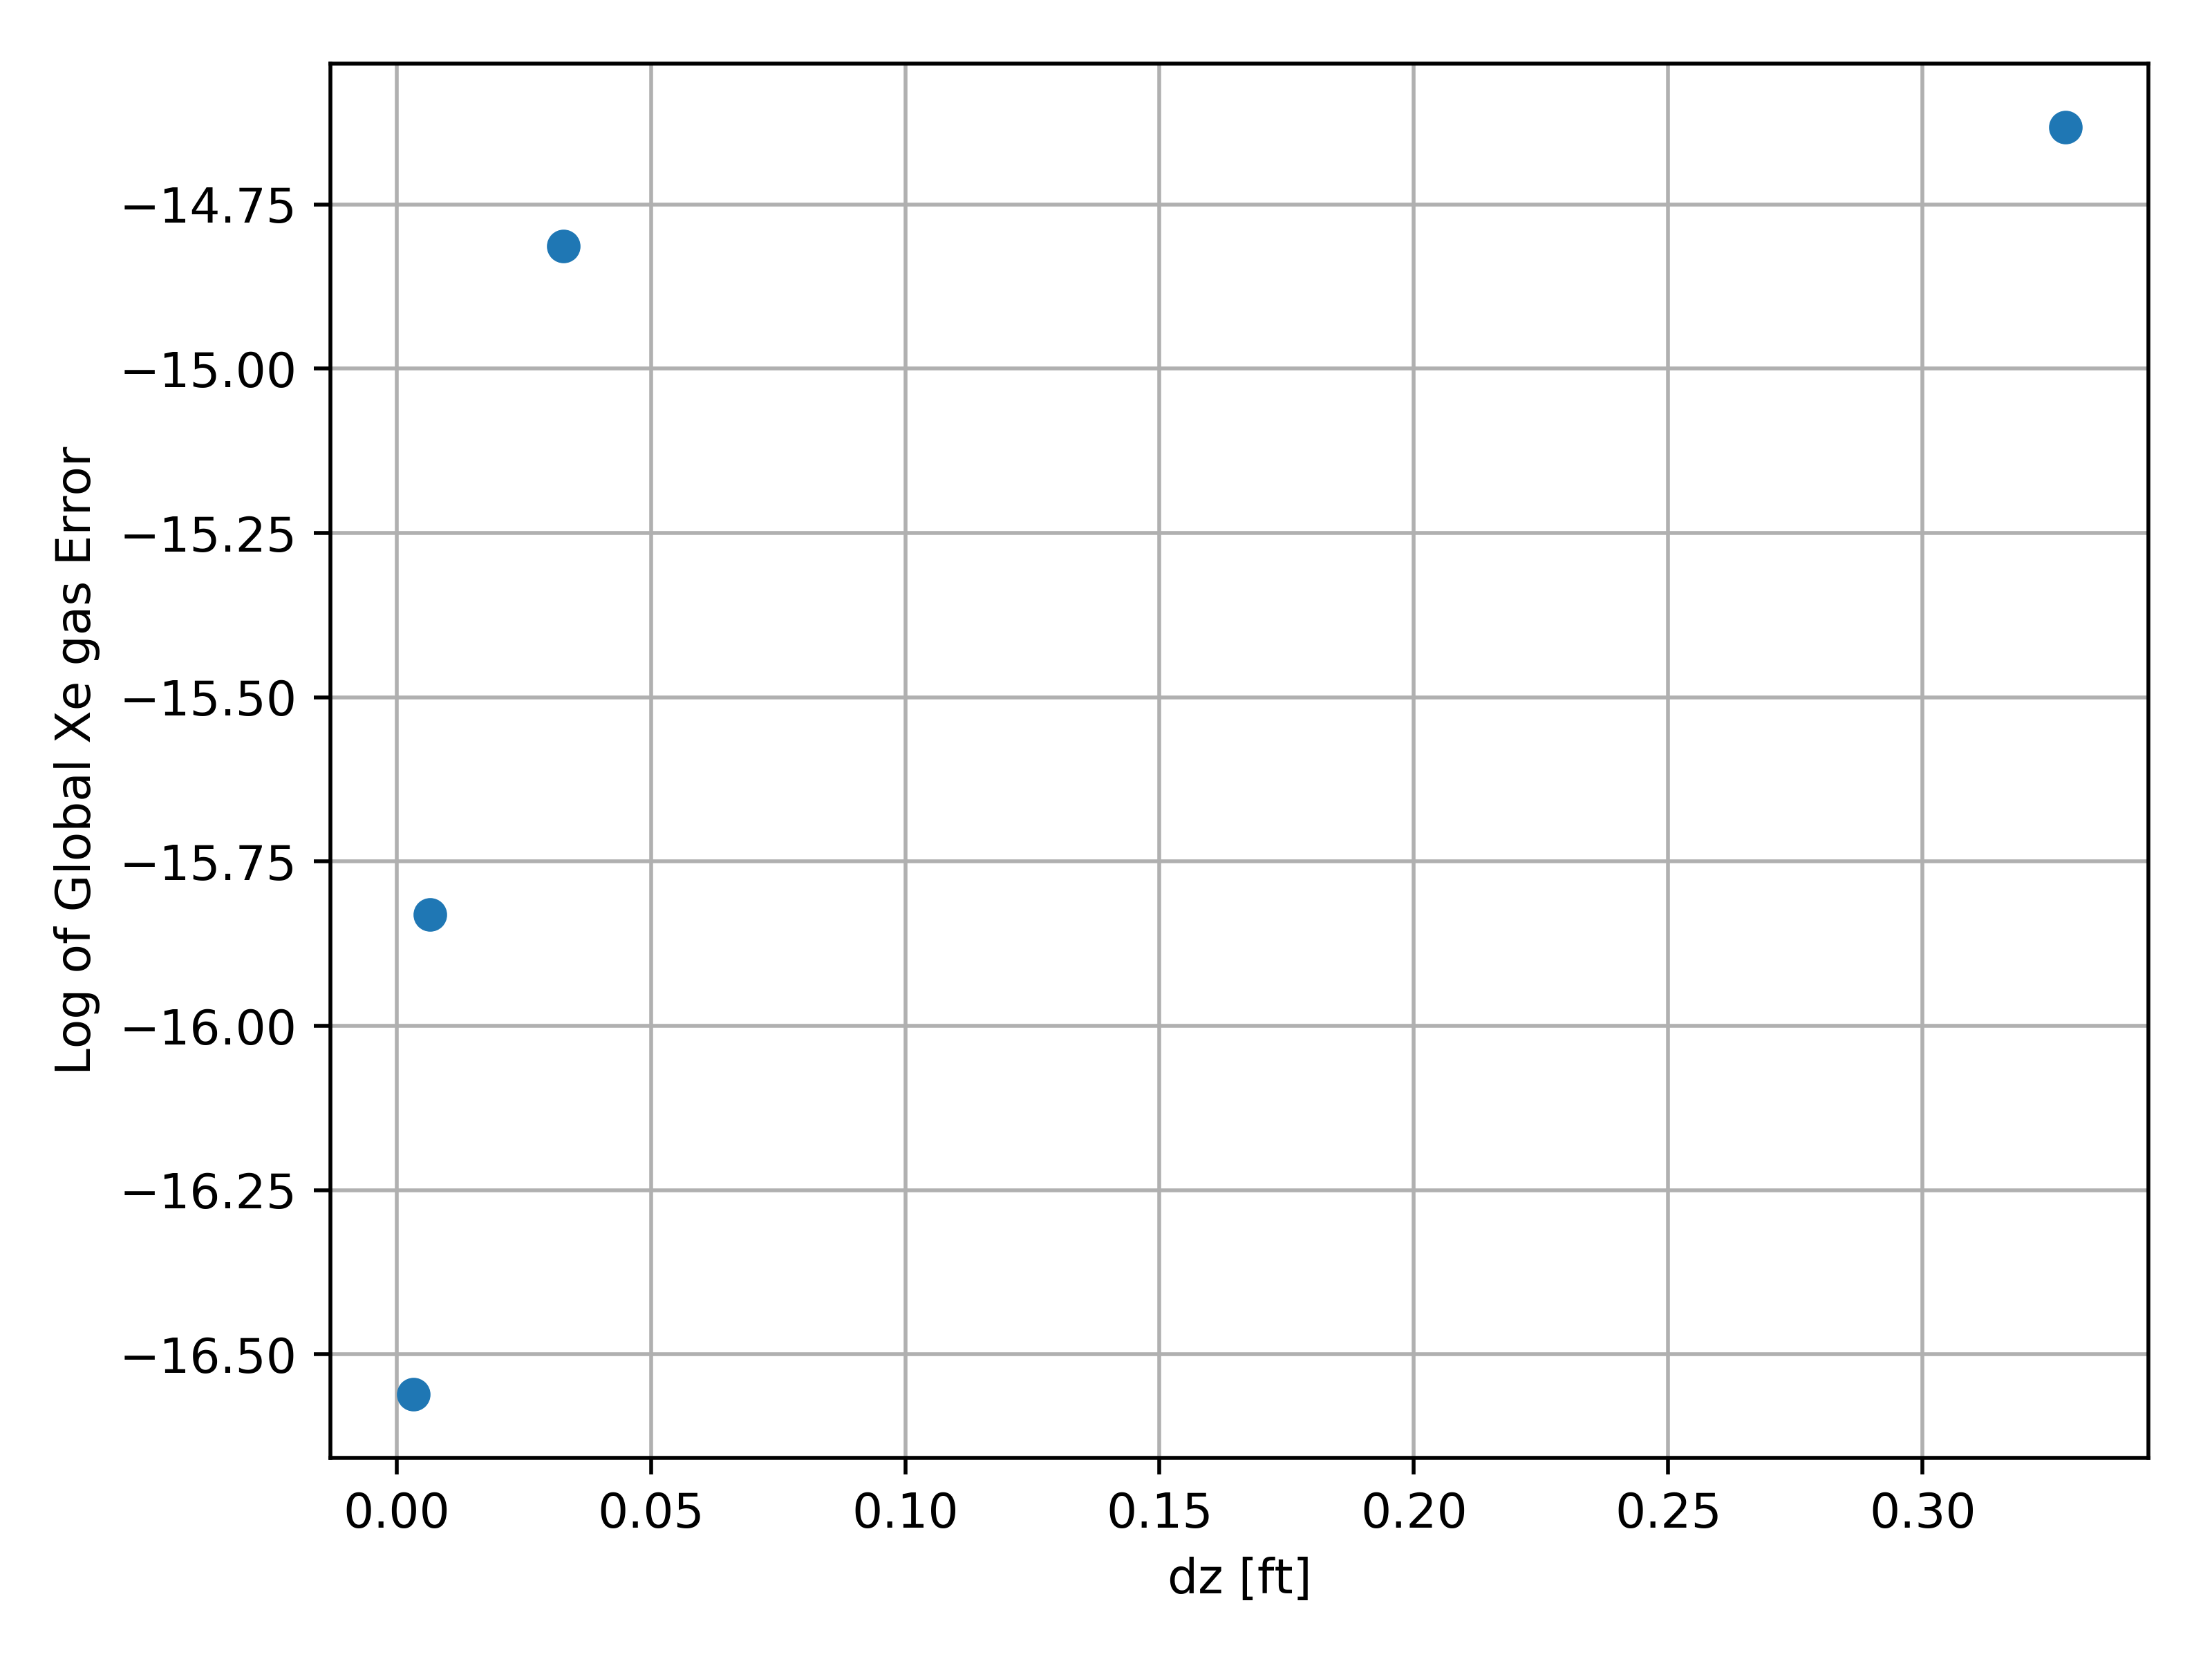
\includegraphics[width=.9\linewidth]{images/transportedSpeciesIntAreaXeLiqError.png}
  \captionof{figure}{Xenon liquid error vs mesh size}
  \label{fig:IntArea_source_xe_liq_error}
\end{minipage}
\end{figure}
\FloatBarrier
\newpage

\subsection{Bubble and Species Removal}
Gas removal was defined in \ref{ch:bubble_BC} to be a removal efficiency multiplied by the incoming flow rate of gas in the cell.  This problem consist of two channels each with 10 axial levels, shown in Figure
\ref{fig:MultiChanBubRemoval_problem}. Xenon and Helium gas bubbles are injected at the bottom of both channels in the first level. Velocity in the axial direction brings the species up and out of the channel. A velocity component is added between the channels and 1/2 the velocity in the axial direction. This causes species to migrate from channel one into channel two. In the seventh level of the second channel 80\% of the bubbles are removed from the channel, bringing with it 80\% of the species in the bubble. 

 Once the problem is run to steady state, a simple mass balance around the removal cell is used to ensure removal is properly working. From simplicity the mass flow rate coming from the bottom of the removal cell is one, from the left is two and leaving the top is three. 
 
\begin{equation}
    \dot{m_{3}} = \dot{m_{1}} + \dot{m_{2}}
    \label{eq:bubbleRemoval_mass_balance}
\end{equation}

Using the following relations between mass flow rate, flux, area and concentration, Equation \ref{eq:bubbleRemoval_mass_balance} is solved for the concentration in the removal cell.

\begin{equation}
    m_{3} = v_{z}C_{3}A_{3}; \quad m_{2} = 0.5v_{z}C_{2}A_{2}(1-S_{eff}); \quad m_{1} = v_{z}C_{1}A_{1}(1-S_{eff})
\end{equation}

Solving equation \ref{eq:bubbleRemoval_mass_balance} for the concentration in the removal cell gives:

\begin{equation}
    C_{removal} = (1-S_{eff}) \bigg[\frac{0.5C_{2}A_{2}}{A_{3}} + C_{1}\bigg]
\end{equation}

Figures \ref{fig:XeGasHeatMap}, \ref{fig:XeliqHeatMap} and \ref{fig:IntAreaConHeatMap} show the density of xenon in the gas bubbles, xenon in the liquid and interfacial area concentration respectively.  All three variables show migration from channel one to channel two due to the velocity component in the lateral direction. Both the concentrations for xenon in the gas and interfacial area drop in the removal cell. After the removal cell, interfiacal area and xenon in the gas both increase from mass transfer, and migration from channel one. 


\FloatBarrier
\newpage

\begin{figure}[ht] 
\centering
\begin{minipage}{.5\textwidth}
  \centering
  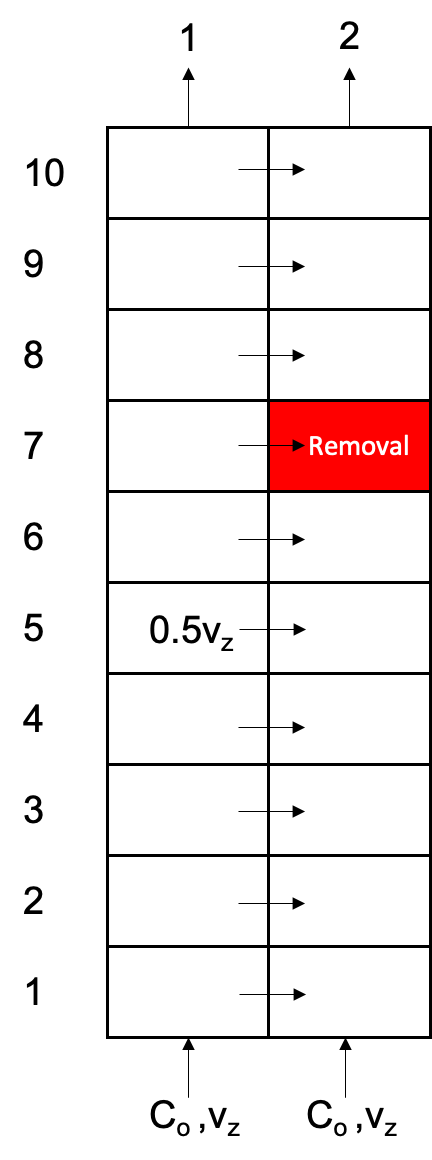
\includegraphics[width=0.78\linewidth]{images/MultiChanBubbleRemoval.png}
  \captionof{figure}{Problem domain}
  \label{fig:MultiChanBubRemoval_problem}
\end{minipage}%
\begin{minipage}{.5\textwidth}
  \centering
  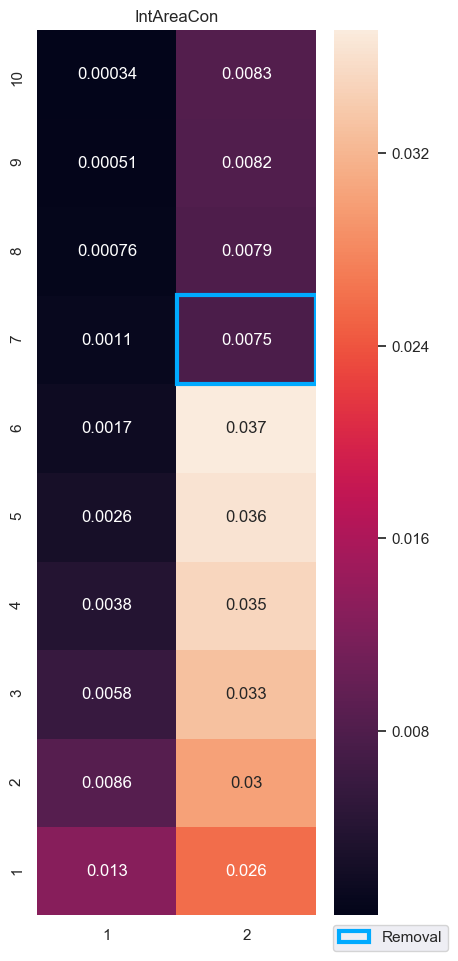
\includegraphics[width=1\linewidth]{images/IntAreaConHeatMap.png}
  \captionof{figure}{Interfacial area concentration}
  \label{fig:IntAreaConHeatMap}
\end{minipage}
\end{figure}

\begin{figure}[ht] 
\centering
\begin{minipage}{.5\textwidth}
  \centering
  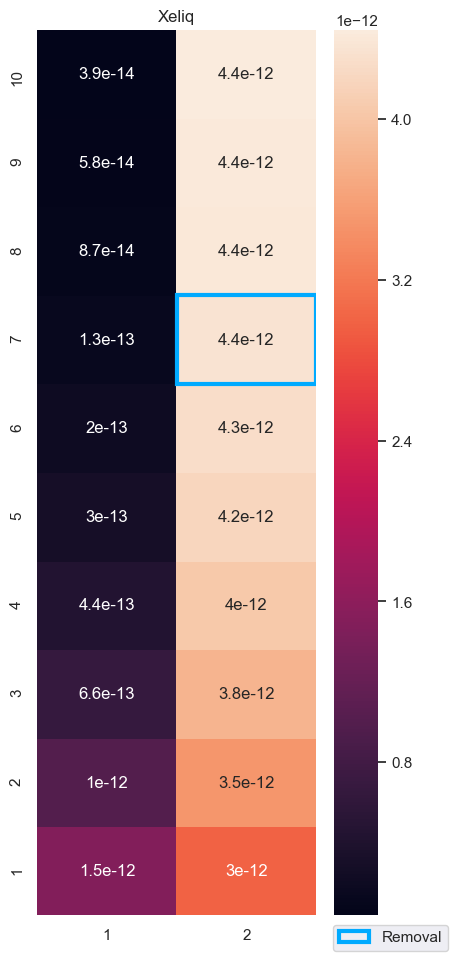
\includegraphics[width=1\linewidth]{images/XeliqHeatMap.png}
  \captionof{figure}{Xenon dissolved in the liquid}
  \label{fig:XeliqHeatMap}
\end{minipage}%
\begin{minipage}{.5\textwidth}
  \centering
  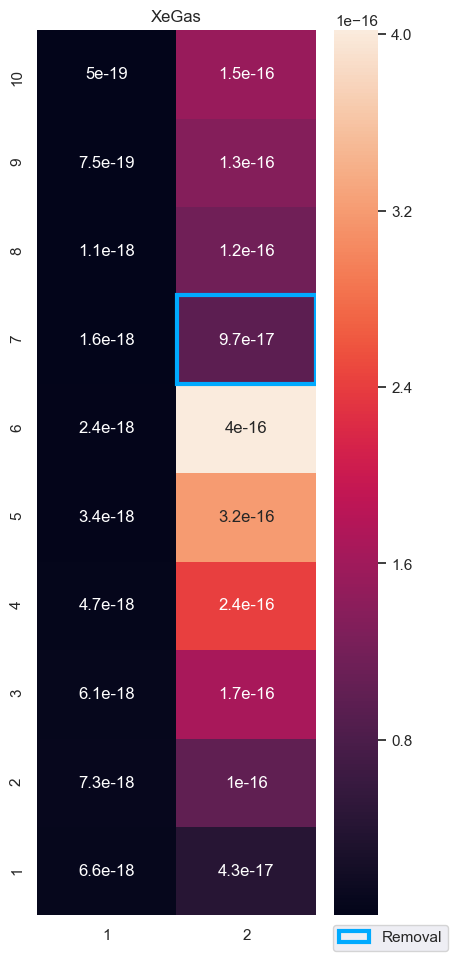
\includegraphics[width=1\linewidth]{images/XeGasHeatMap.png}
  \captionof{figure}{Xenon is the gas bubbles}
  \label{fig:XeGasHeatMap}
\end{minipage}
\end{figure}

\FloatBarrier
\newpage




\section{Case Studies}
Sections \ref{sec:gen_transport} and \ref{sec:gas_transport} demonstrated that individual components for species transport and multi-phase transport properly work. In this section we will analysis a coupled xenon iodine system, as well as how varying parameters impacts the xenon behavior. A base case is chosen from related MSRE information, then boundary conditions are changed to examine their impact on xenon in the circulating bubbles. 


The governing equations are similar to those in Equations \ref{eq:XenonGeneralDiffEq} and \ref{eq:IodineGeneralDiffEq} but with the addition of mass transfer from xenon in the liquid to xenon in the gas. These Equations are shown in \ref{eq:XenonLiqCaseStudyDiffEq} through \ref{eq:IodineLiqCaseStudyDiffEq}. A total of five species will be modeled, two for xenon, two for helium and one for iodine. One of the xenon species will denote the xenon dissolved in the molten salt and the other will denote the xenon trapped in the helium bubbles, the same goes for helium. Iodine is assumed not to migrate into the circulating void. Table \ref{tab:simple_loop_test_parameters} gives the problem parameters for the base case. The average void experienced in the MSRE was between 0.02 and 0.04 \cite{engel1971}, the Helium gas injection rate was determined using these values.

The simple loop is a scaled down version of an MSRE model, shown in Figure \ref{fig:simple_loop}. This model is broken down into six sections each with their own color code. Red is the core region, gold is the upper plenum which houses the pump. White is the heat exchanger, blue is the turn around elbow. Purple is the down comer, and black is the core inlet. 

\vspace{12.7mm} %5mm vertical space

\begin{figure}[ht]
  \centering
  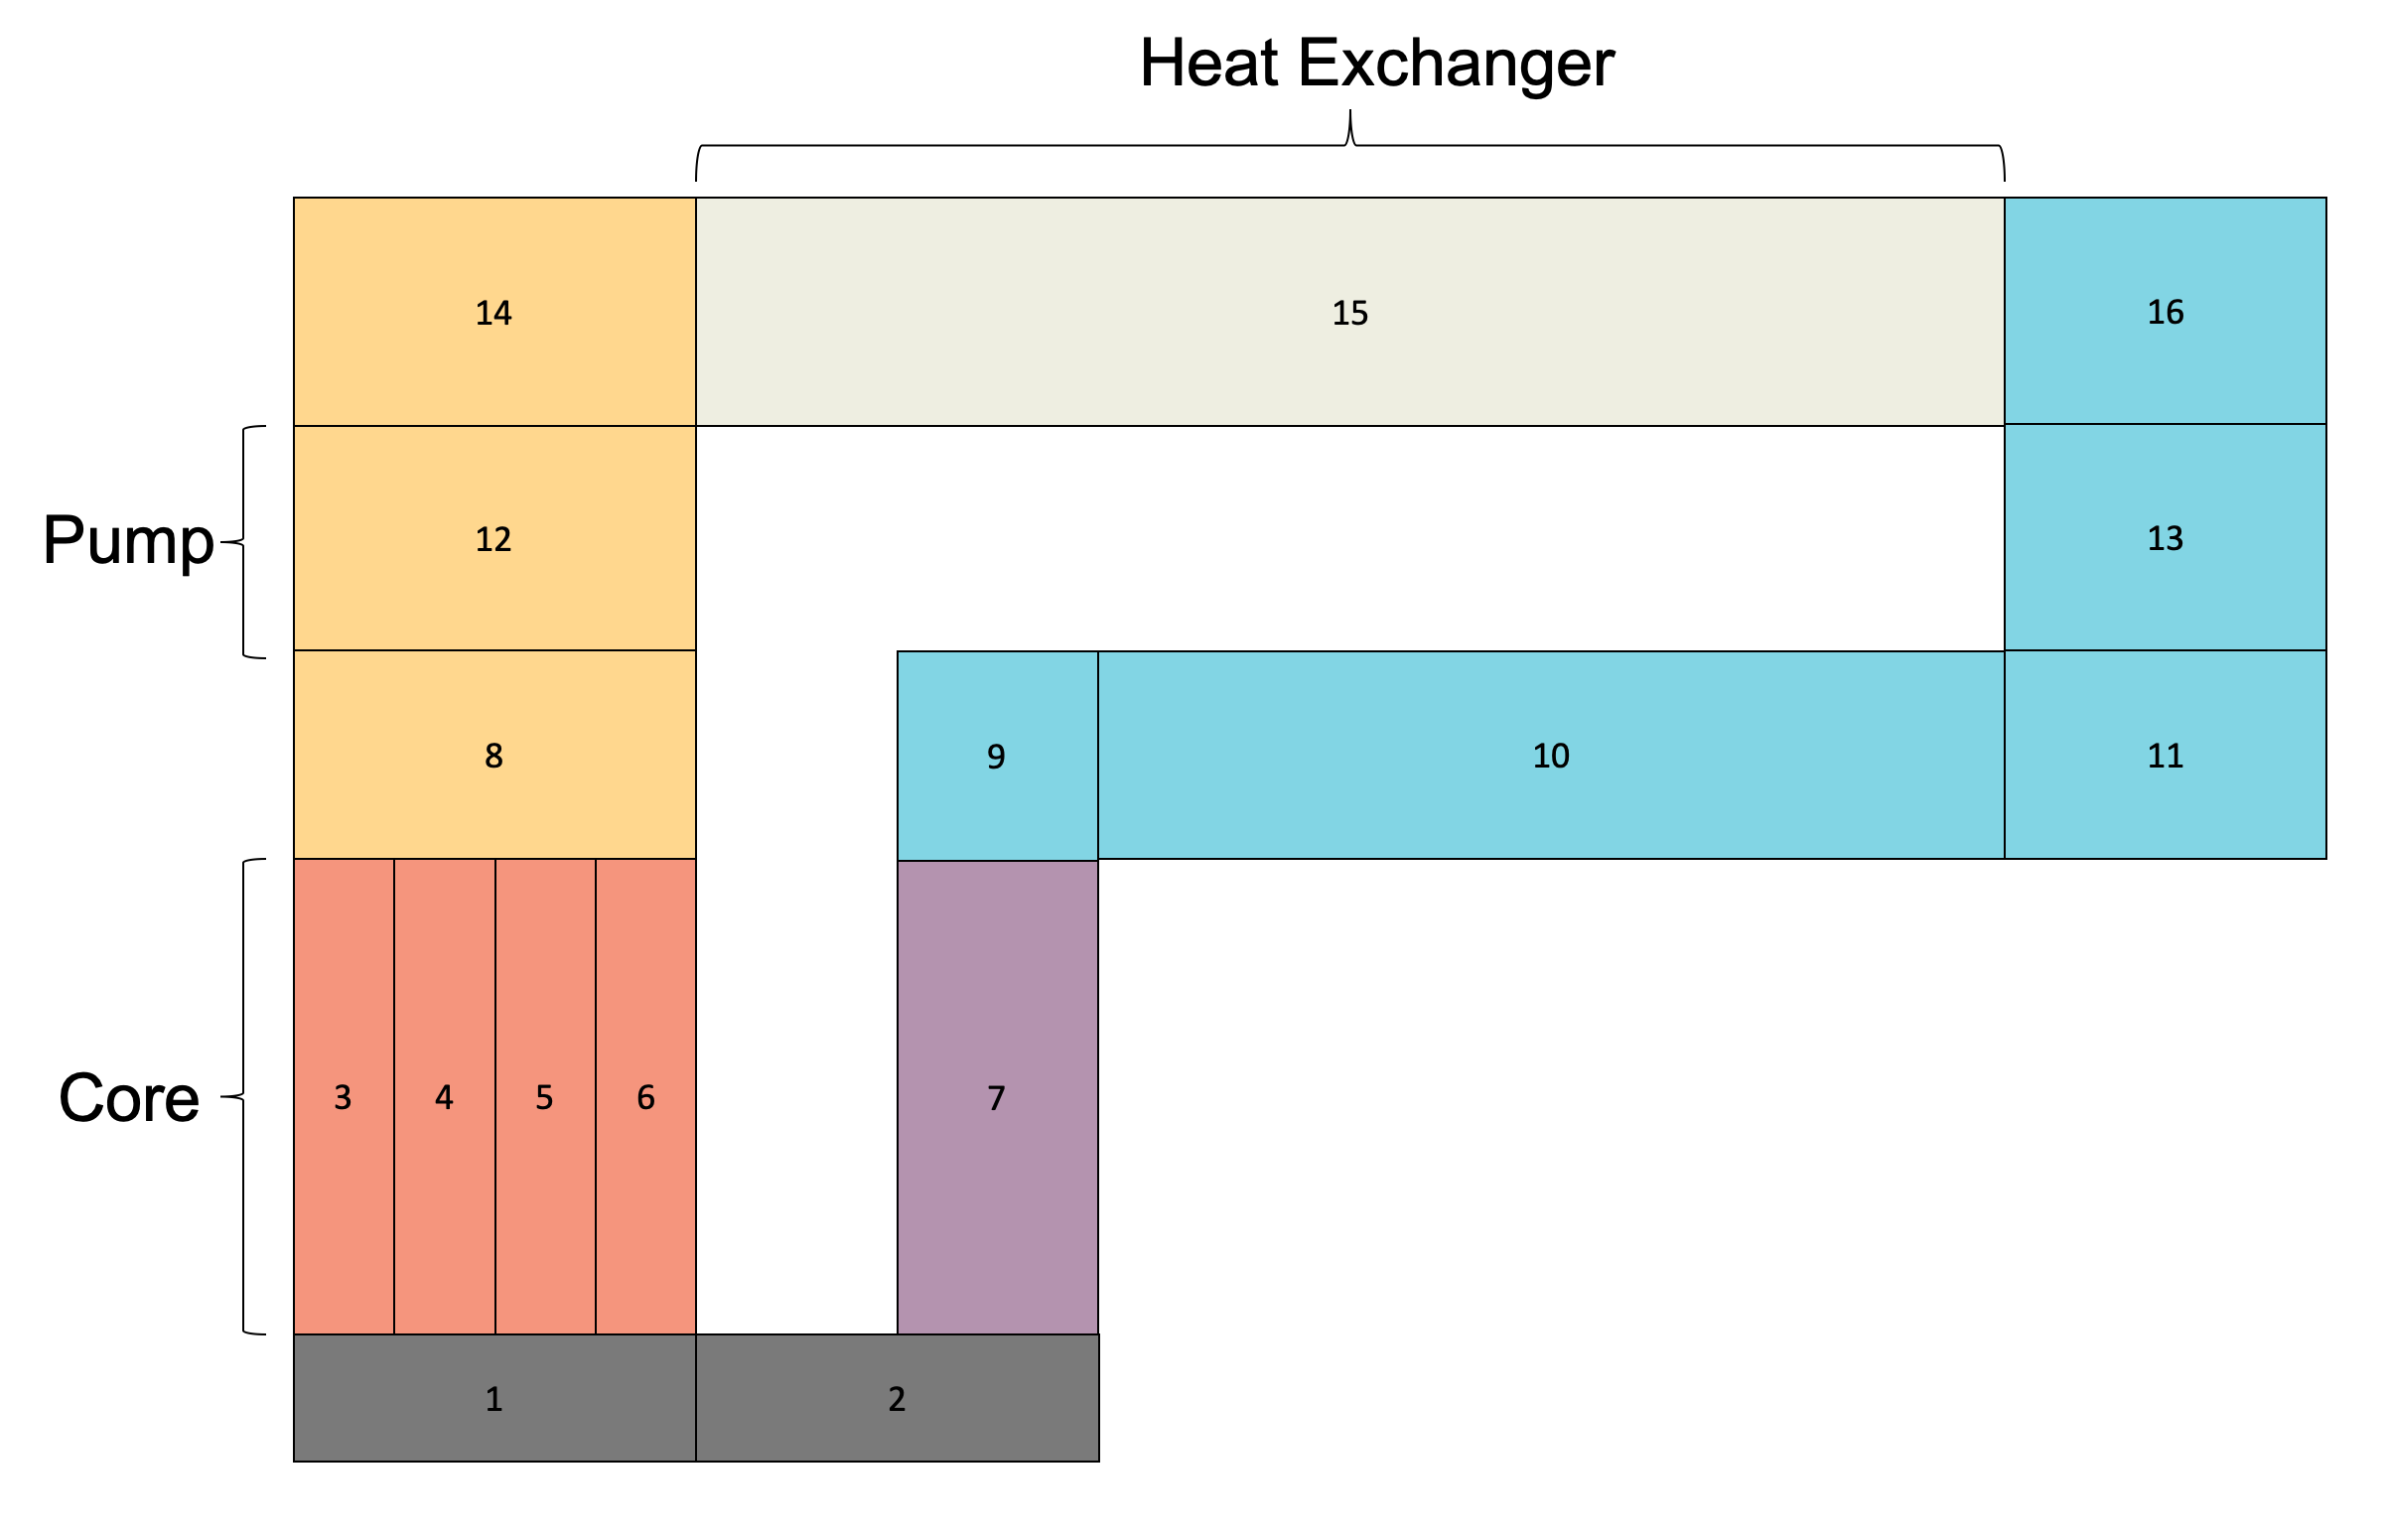
\includegraphics[width=5in]{images/simple_loop.png}\\
  \caption{Simple loop diagram}
  \label{fig:simple_loop}
\end{figure}

\begin{table}[htbp!]
   \caption{\label{tab:simple_loop_test_parameters} Base case parameters}
   \centering
   \begin{tabular}{lll}
   \hline
   \textbf{Parameter} & \textbf{Value} & \textbf{Unit} \\
   \hline 
   $\gamma_{I}$ & $6.3033$ \cite{cole2019}& $\%$ \\ [1ex]
   $\gamma_{Xe}$ & 0.2468 \cite{cole2019}& \% \\ [1ex]
   $\Sigma_{f}$ & 9.7532E-1 \cite{cole2019}& 1/ft \\ [1ex]
   $\Phi$ & $2.5E16$ \cite{nestor1960}& $n/ft^{2}/s$ \\ [1ex]
   $\lambda_{Xe}$ & 2.11E-5 \cite{cole2019}& 1/s\\ [1ex]
   $\lambda_{I}$ & 2.9306E-5 \cite{cole2019}& 1/s  \\ [1ex]
   $M_{Xe}$ & 135.0 & lbm/mol\\ [1ex]
   $M_{I}$ & 135.0 & lbm/mol \\ [1ex]
   $M_{He}$ & 4.0 & lbm/mol \\ [1ex]
   $k_{Xe}$ & 2.0 \cite{houtzeel1967} & ft/hr\\ [1ex]
   $k_{He}$ & 4.0 \cite{engel1971} & ft/hr \\ [1ex]
   $H_{Xe}$ & 2.75E-9 \cite{houtzeel1967} & mole/cm${}^{3}$/atm \\ [1ex]
   $H_{He}$ & 1.26E-7 \cite{engel1971} & mole/cm${}^{3}$/atm \\ [1ex]
   $D_{ref}$ & 0.03175${}^{a}$  & cm \\ [1ex]
   He injection rate & 2.0E-5 & moles/s \\ [1ex]
   Removal efficiency & 0.99 & \% \\ [1ex] 
   $\alpha$ Void fraction & - & - \\ [1ex]
   \hline
      \end{tabular}
    \begin{tablenotes}\footnotesize
   \item[a] This value is the average for the range of bubbles considered in the MSRE 0.0127-0.0508 cm \cite{engel1971}
   \end{tablenotes}

\end{table}

% xenon liq
\begin{equation}
\begin{split}
    \frac{\partial \rho_{Xe}^{l}}{\partial t} = -\nabla (\rho_{Xe}^{l}v) + \frac{M_{Xe}}{N_{A}(1-\alpha)} \gamma_{Xe}\Sigma_{f}\Phi + \frac{M_{Xe}}{M_{I}}\lambda_{I}\rho_{I} -  \\ \lambda_{Xe}\rho_{Xe} - \sigma_{a}\Phi\rho_{Xe} +   \frac{Ka}{V}\Big[\rho_{Xe}^{*} - \frac{\rho_{Xe}^{l}}{1-\alpha}\Big]
    \label{eq:XenonLiqCaseStudyDiffEq}
\end{split}
\end{equation}

% xenon gas
\begin{equation}
    \frac{\partial \rho_{Xe}^{g}}{\partial t} = -\nabla (\rho_{Xe}^{g}v) + \frac{Ka}{V}\Big[\frac{\rho_{Xe}^{l}}{1-\alpha}  - \rho_{Xe}^{*}\Big]
    \label{eq:XenonGasCaseStudyDiffEq}
\end{equation}

% helium gas
\begin{equation}
    \frac{\partial \rho_{He}^{g}}{\partial t} = -\nabla (\rho_{He}^{g}v) + \frac{Ka}{V}\Big[\frac{\rho_{He}^{l}}{1-\alpha}  - \rho_{He}^{*}\Big]
    \label{eq:HeGasCaseStudyDiffEq}
\end{equation}

% helium liquid
\begin{equation}
    \frac{\partial \rho_{He}^{l}}{\partial t} = -\nabla (\rho_{He}^{l}v) + \frac{Ka}{V}\Big[ \rho_{He}^{*} - \frac{\rho_{He}^{l}}{1-\alpha}\Big]
    \label{eq:heliumLiqCaseStudyDiffEq}
\end{equation}

% iodine liquid
\begin{equation}
    \frac{\partial \rho_{I}^{l}}{\partial t} = -\nabla (\rho_{I}^{l}v) + \frac{M_{I}}{N_{A}(1-\alpha)} \gamma_{I}\Sigma_{f}\Phi - \lambda_{I}\rho_{I}
    \label{eq:IodineLiqCaseStudyDiffEq}
\end{equation}

\subsection{Base Case Results}
All cases hear forth are ran using the explicit method for a run time of 1000 seconds (dt=1.0E-2) to allow the system to reach steady state. quantities of xenon dissolved in the liquid and trapped in the gas bubbles will be in atoms per foot cubed. In nuclear engineering it is common to use atomic densities. Helium both in the bubbles and dissolved in the liquid will be in moles per foot cubed. Along with the for mentioned variables, interfacial area, bubble diameter, void and percent xenon in the bubbles are also analysed. These variables will be used at the metrics for comparing the relative cases. Shown in Figure \ref{fig:BaseCaseTemp} to \ref{fig:BaseCaseXePercent} are the base case results.

\vspace{12.7mm} %5mm vertical space

% Temp and Press
\begin{figure}[ht] 
\centering
\begin{minipage}{.5\textwidth}
  \centering
  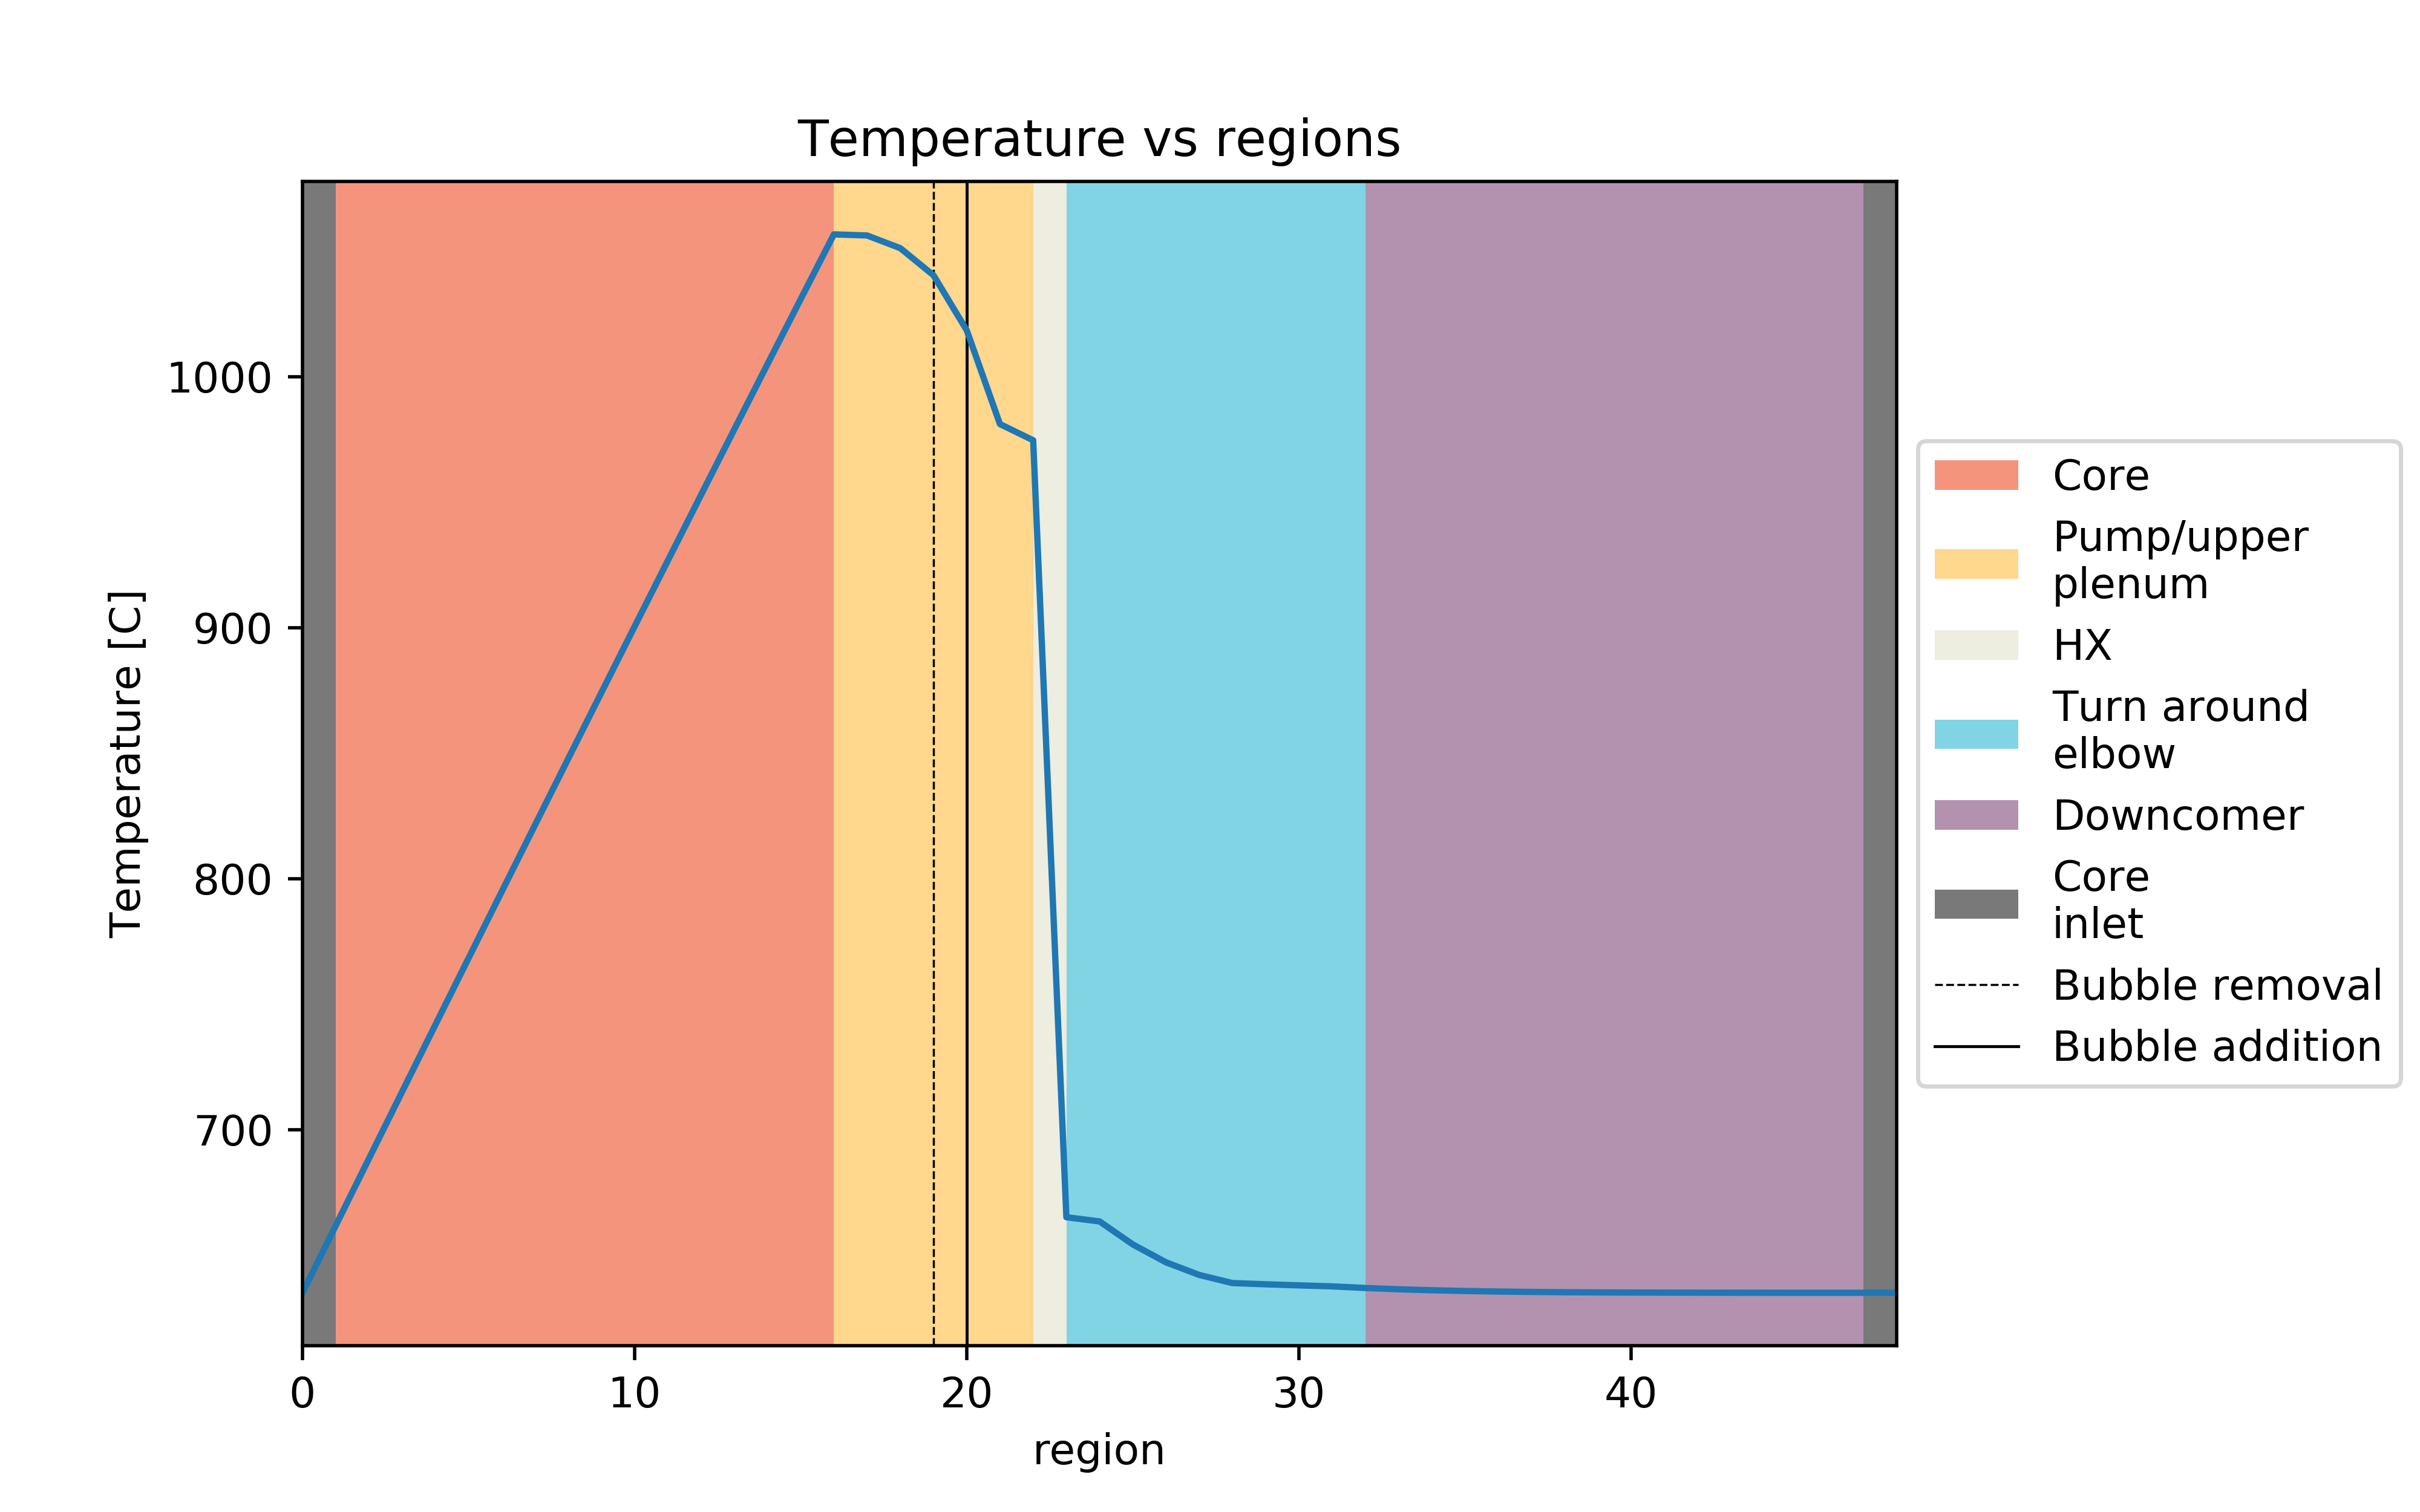
\includegraphics[width=1.0\linewidth]{images/BaseCaseTemperature.png}
  \captionof{figure}{Temperature}
  \label{fig:BaseCaseTemp}
\end{minipage}%
\begin{minipage}{.5\textwidth}
  \centering
  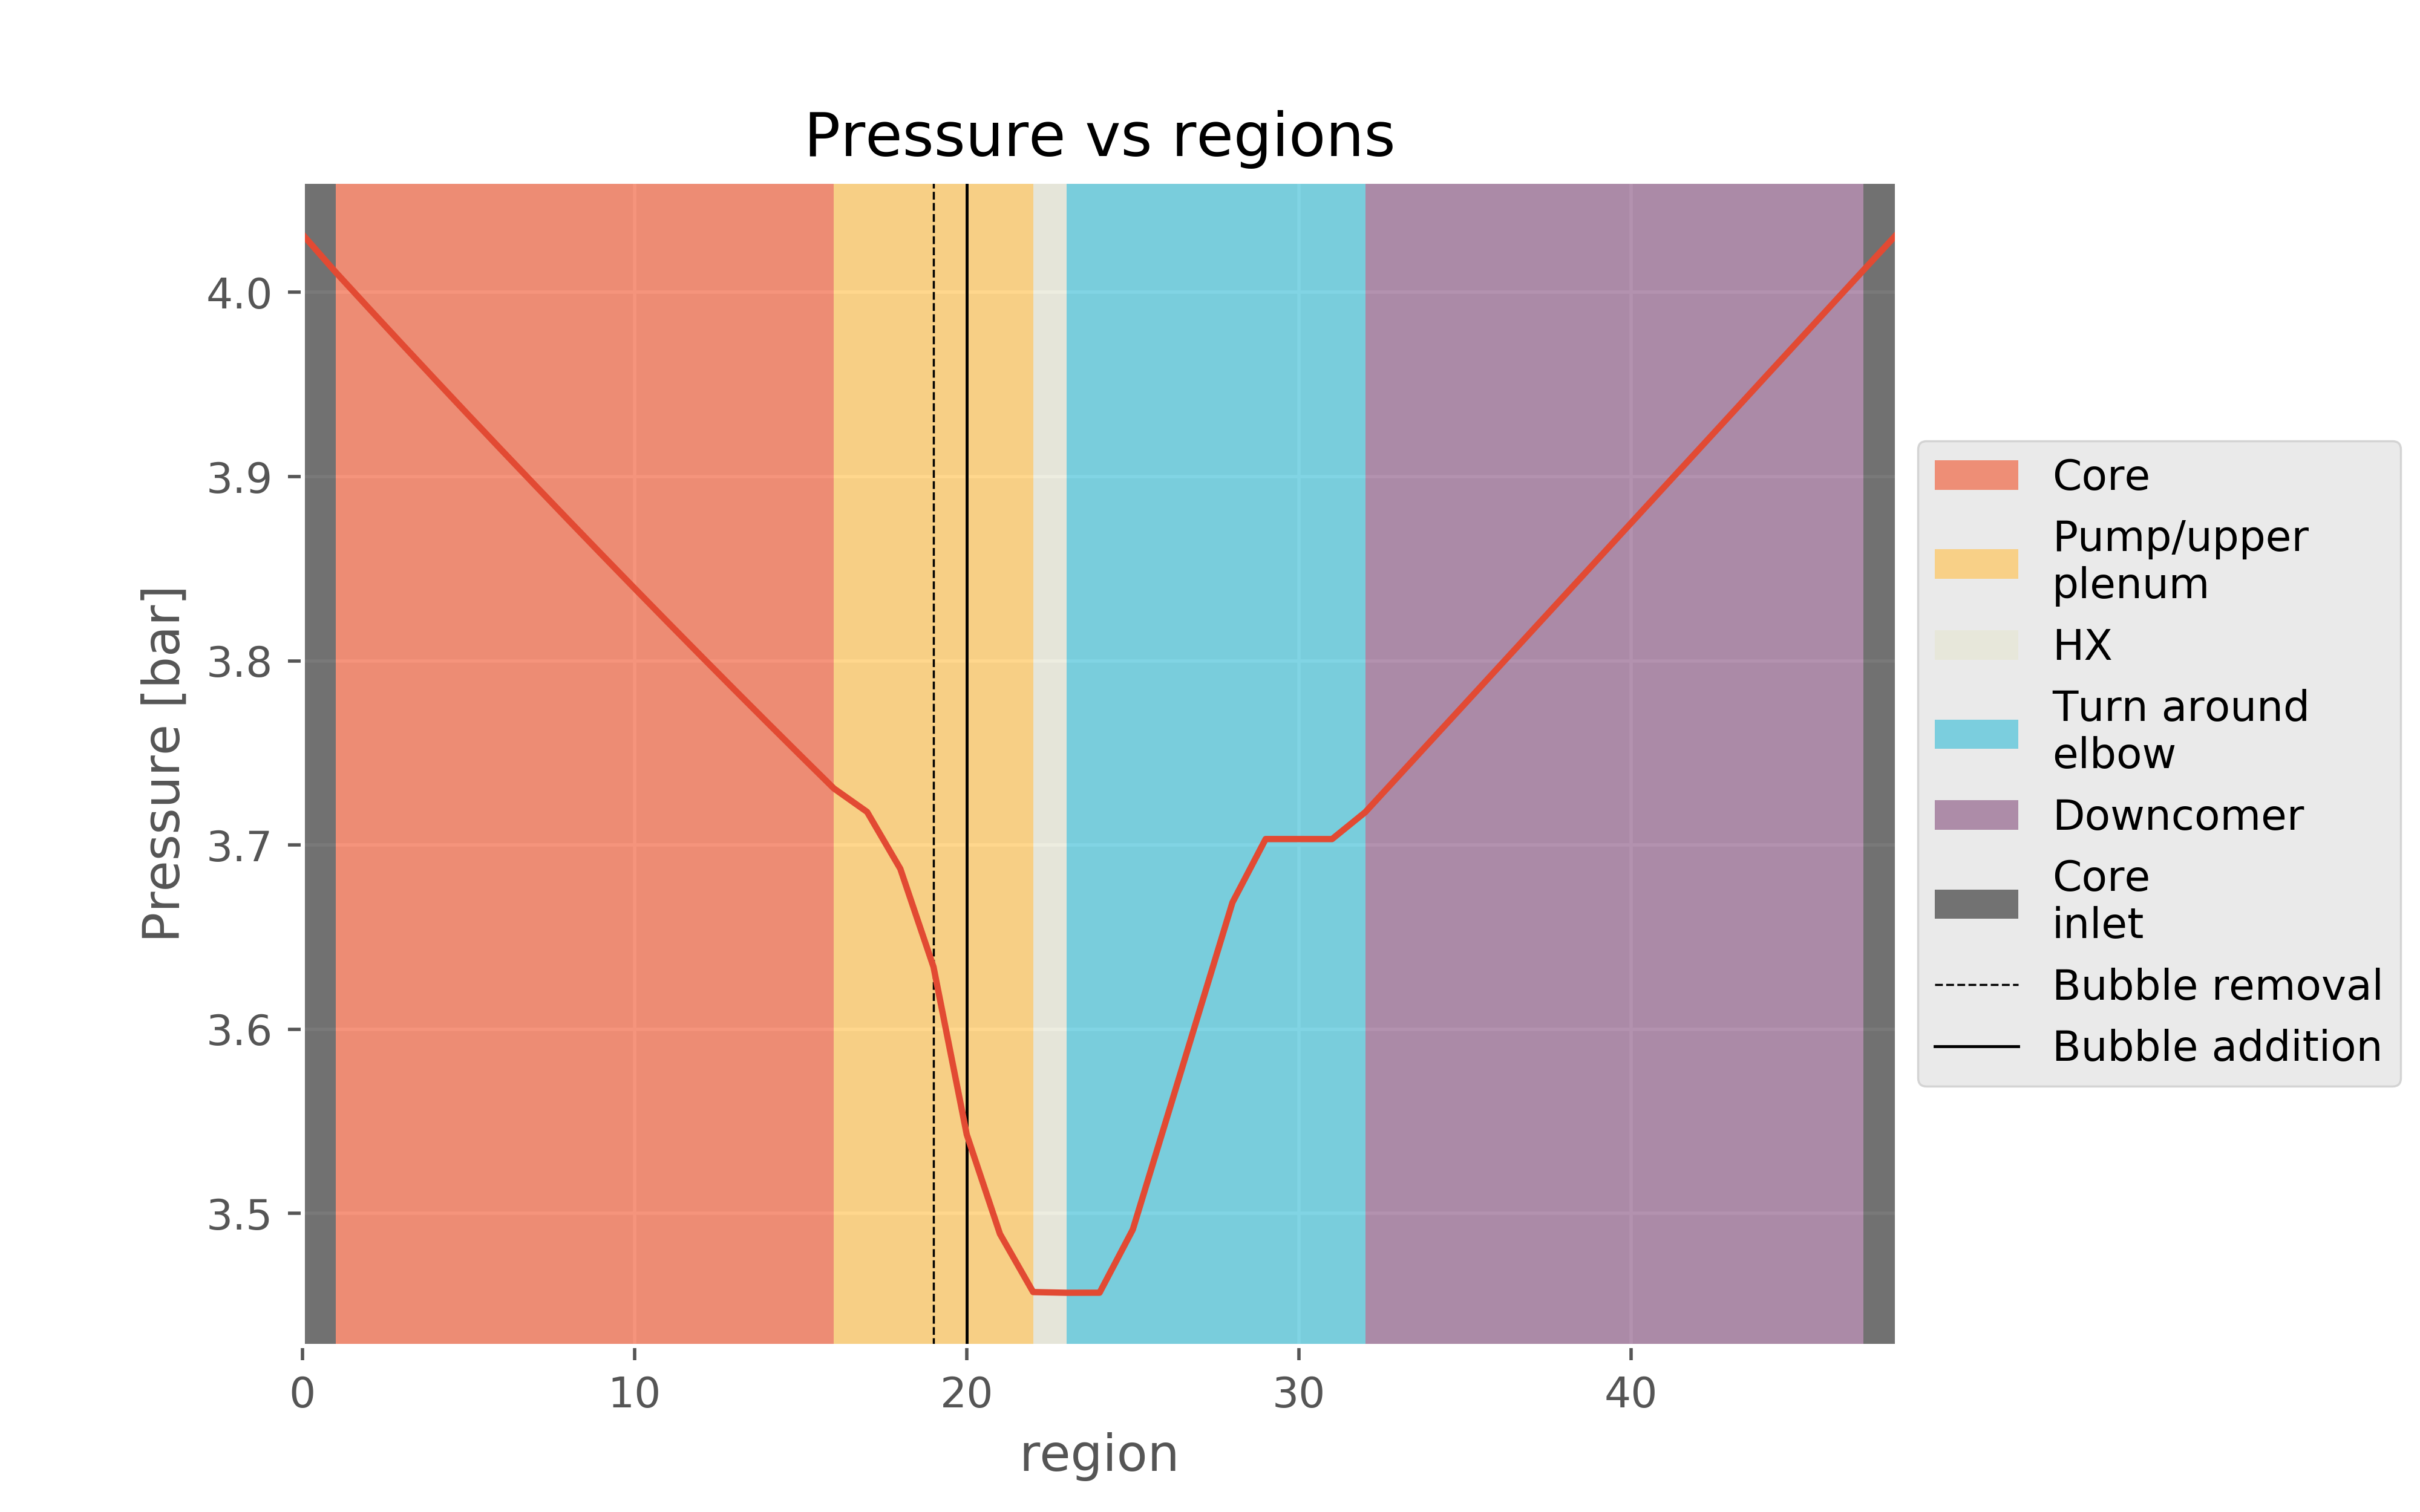
\includegraphics[width=1.0\linewidth]{images/BaseCasePressure.png}
  \captionof{figure}{Pressure}
  \label{fig:BaseCasePress}
\end{minipage}
\end{figure}

% void and diameter
\begin{figure}[ht] 
\centering
\begin{minipage}{.5\textwidth}
  \centering
  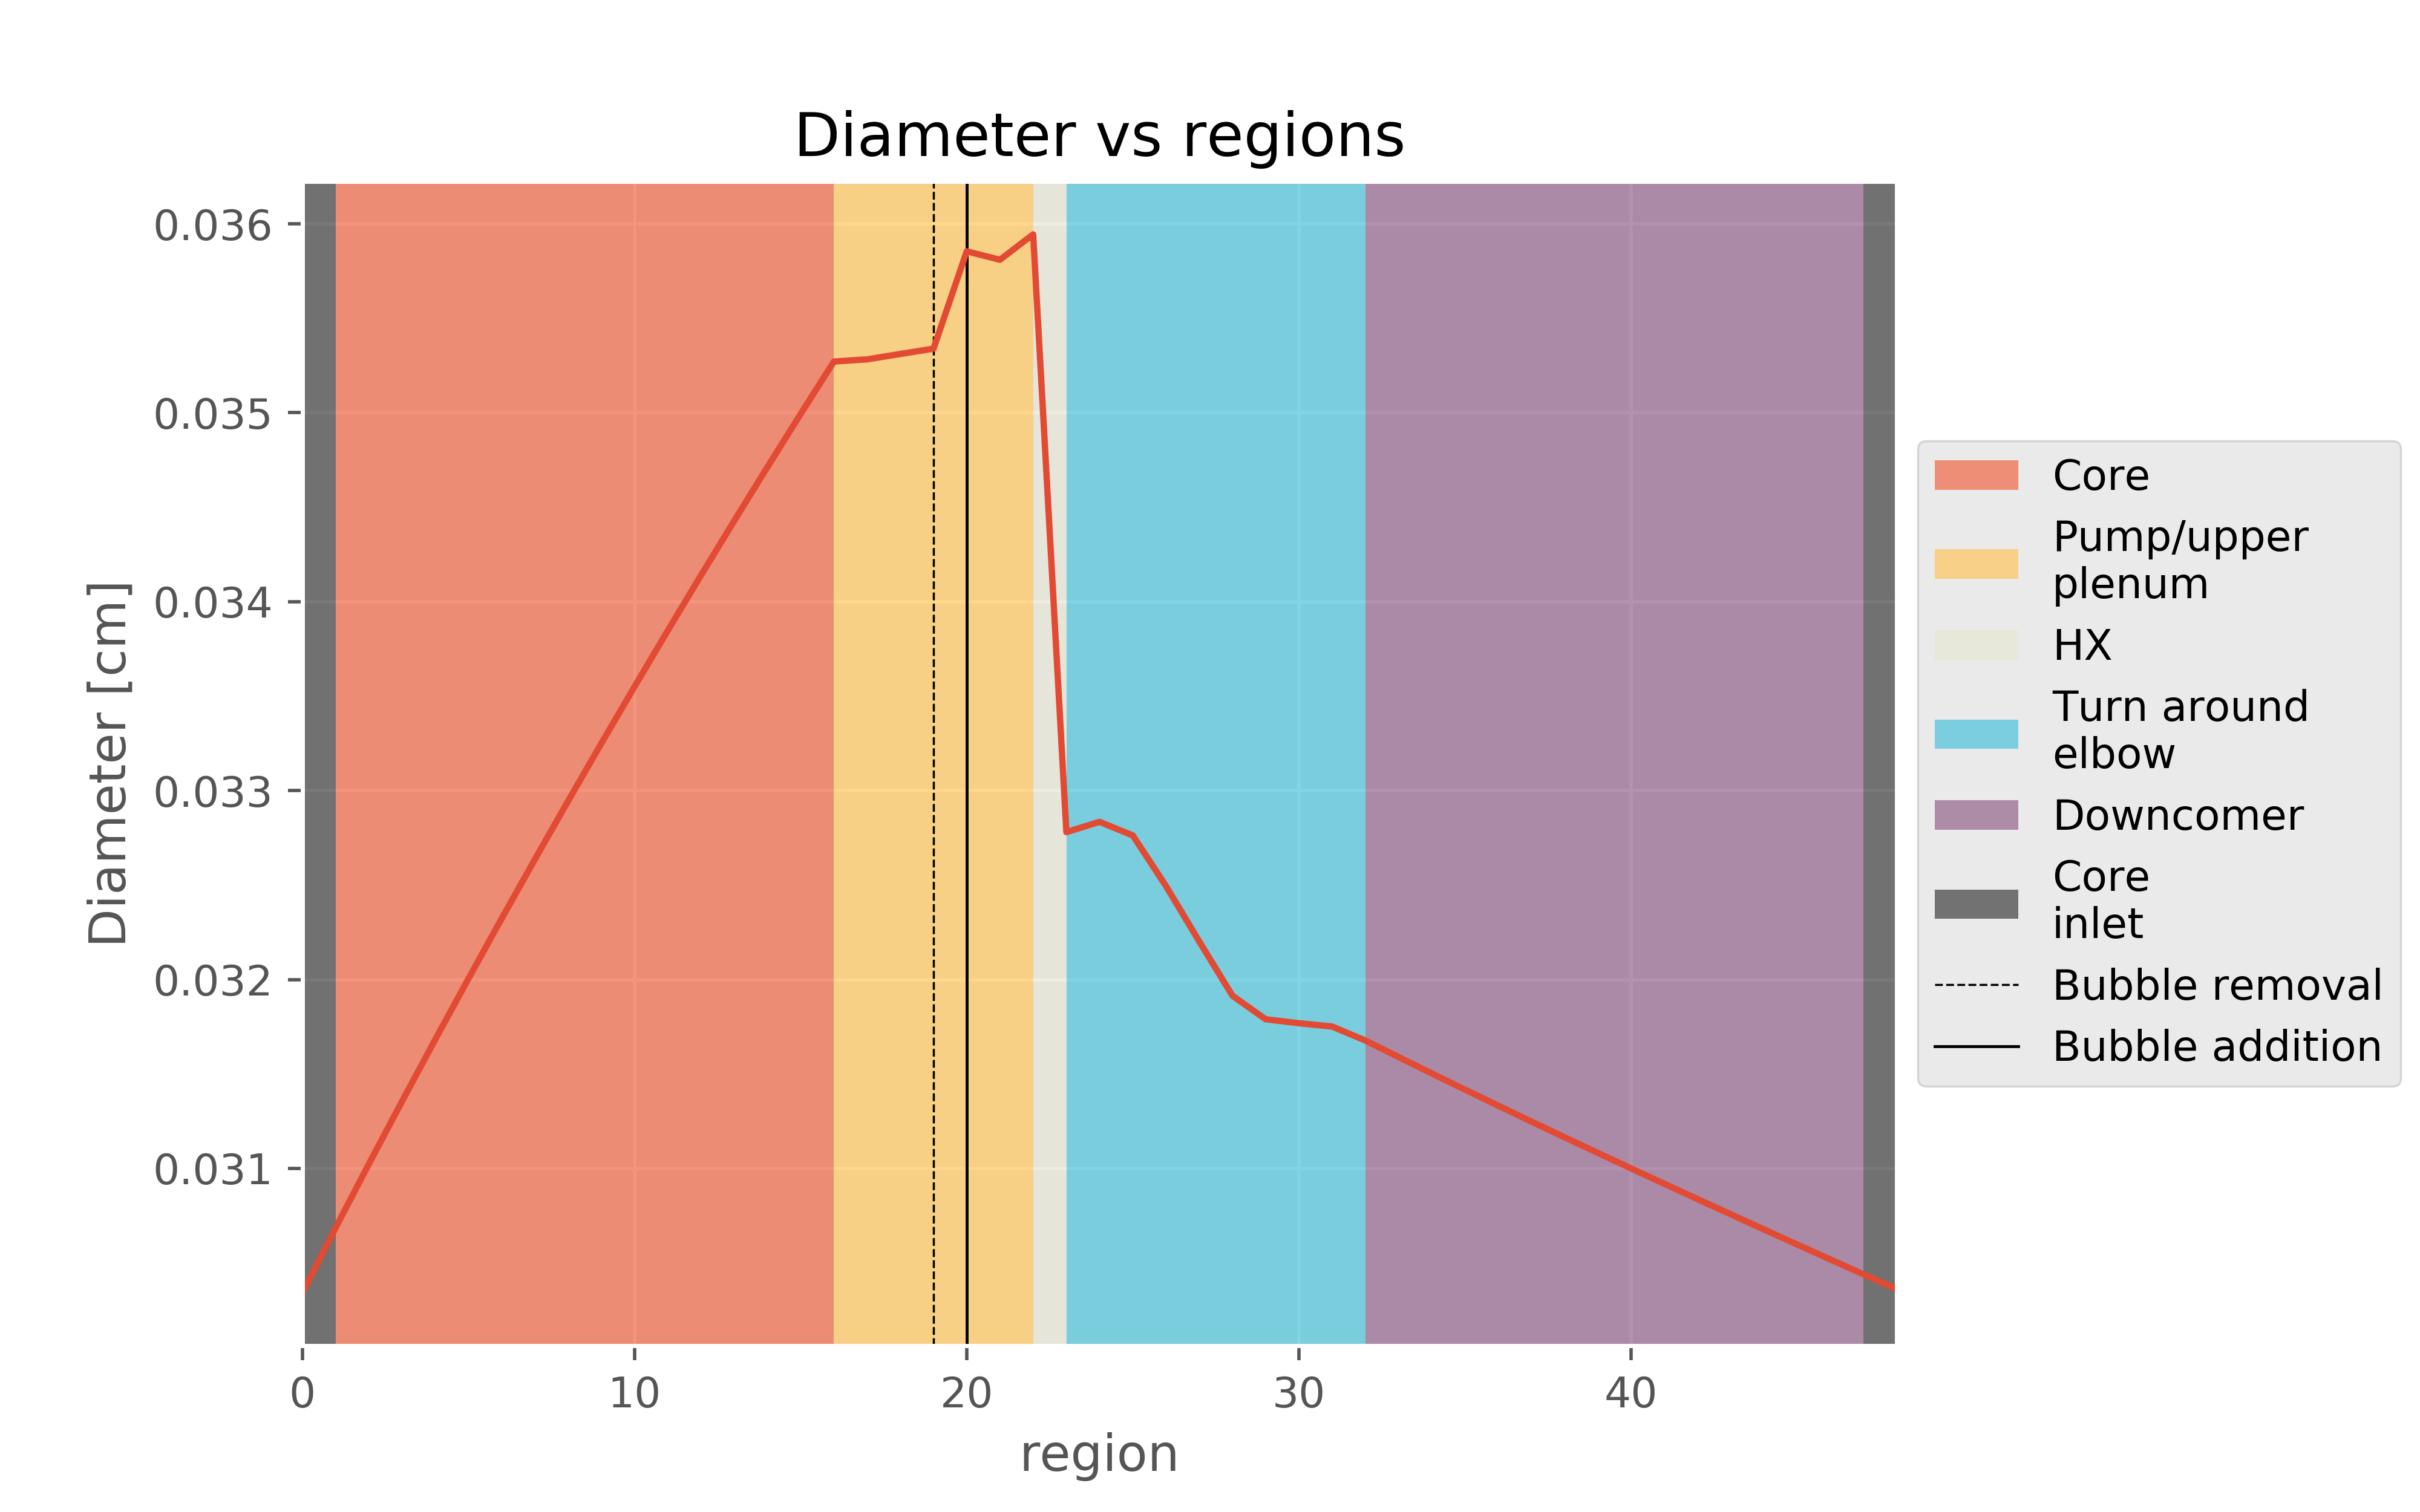
\includegraphics[width=1.0\linewidth]{images/BaseCaseDiameter.png}
  \captionof{figure}{Bubble diameter}
  \label{fig:BaseCaseDia}
\end{minipage}%
\begin{minipage}{.5\textwidth}
  \centering
  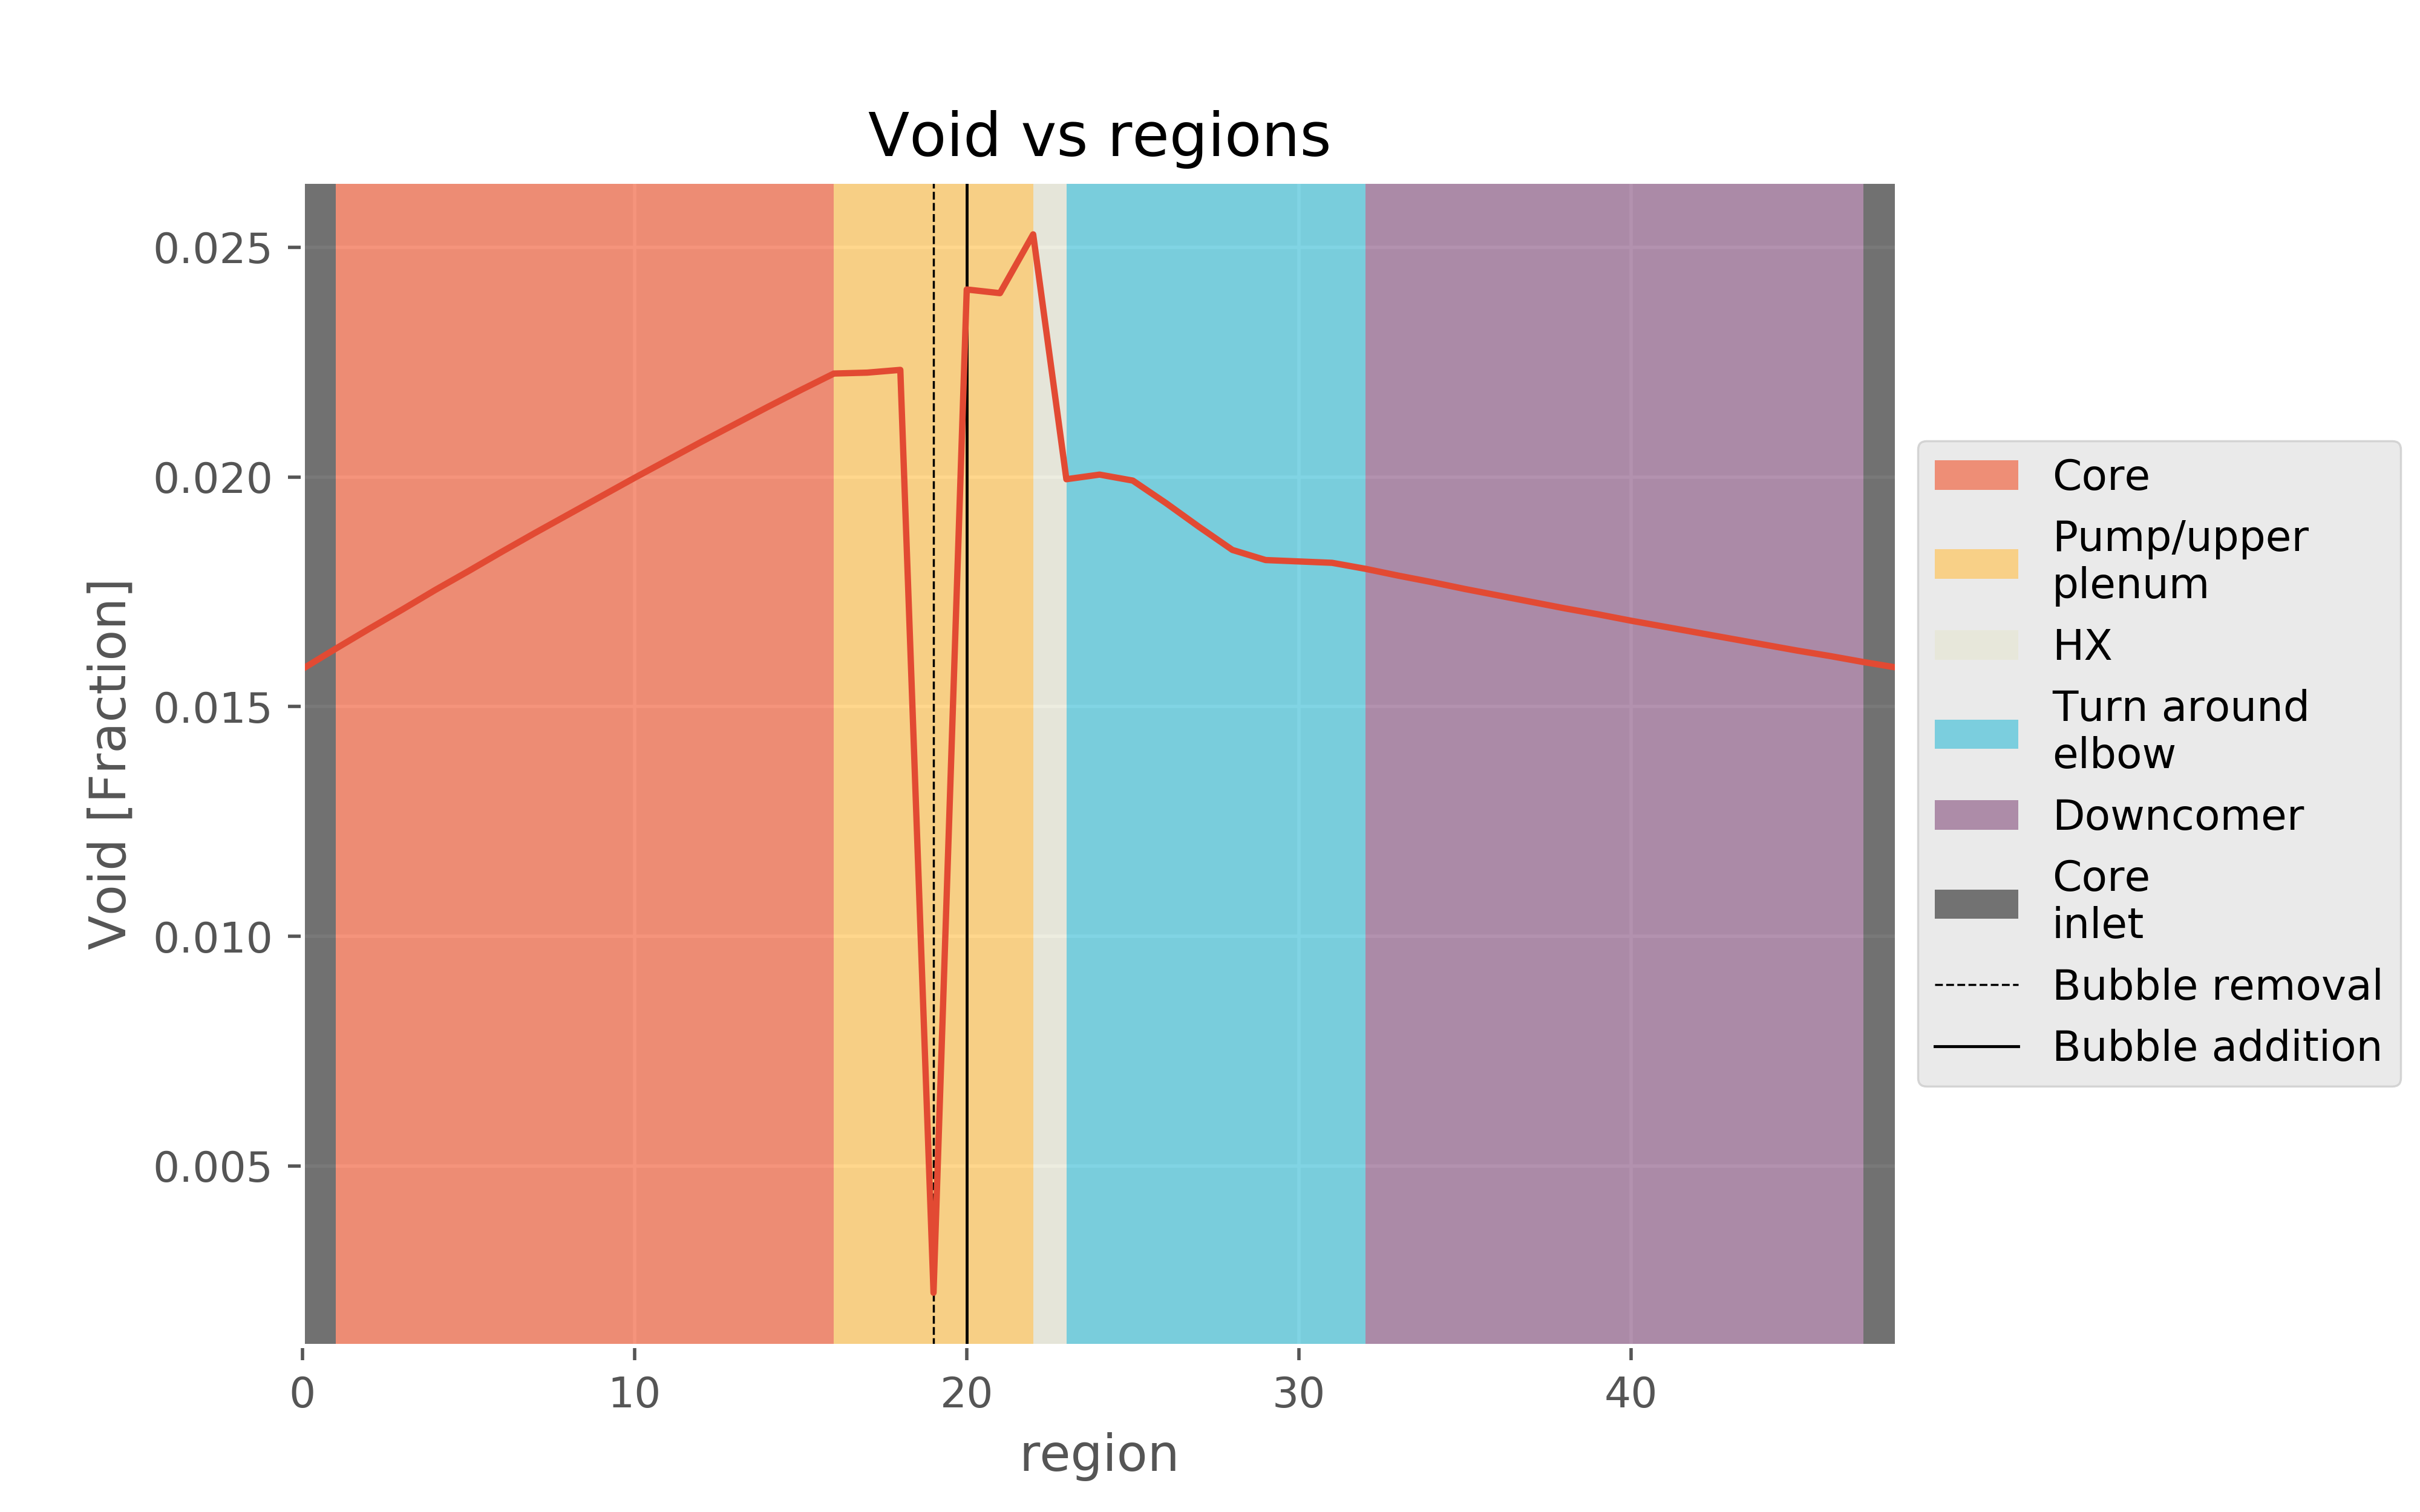
\includegraphics[width=1.0\linewidth]{images/BaseCaseVoid.png}
  \captionof{figure}{Void fraction}
  \label{fig:BaseCaseVoid}
\end{minipage}
\end{figure}

% IntArea and Iodine
\begin{figure}[ht] 
\centering
\begin{minipage}{.5\textwidth}
  \centering
  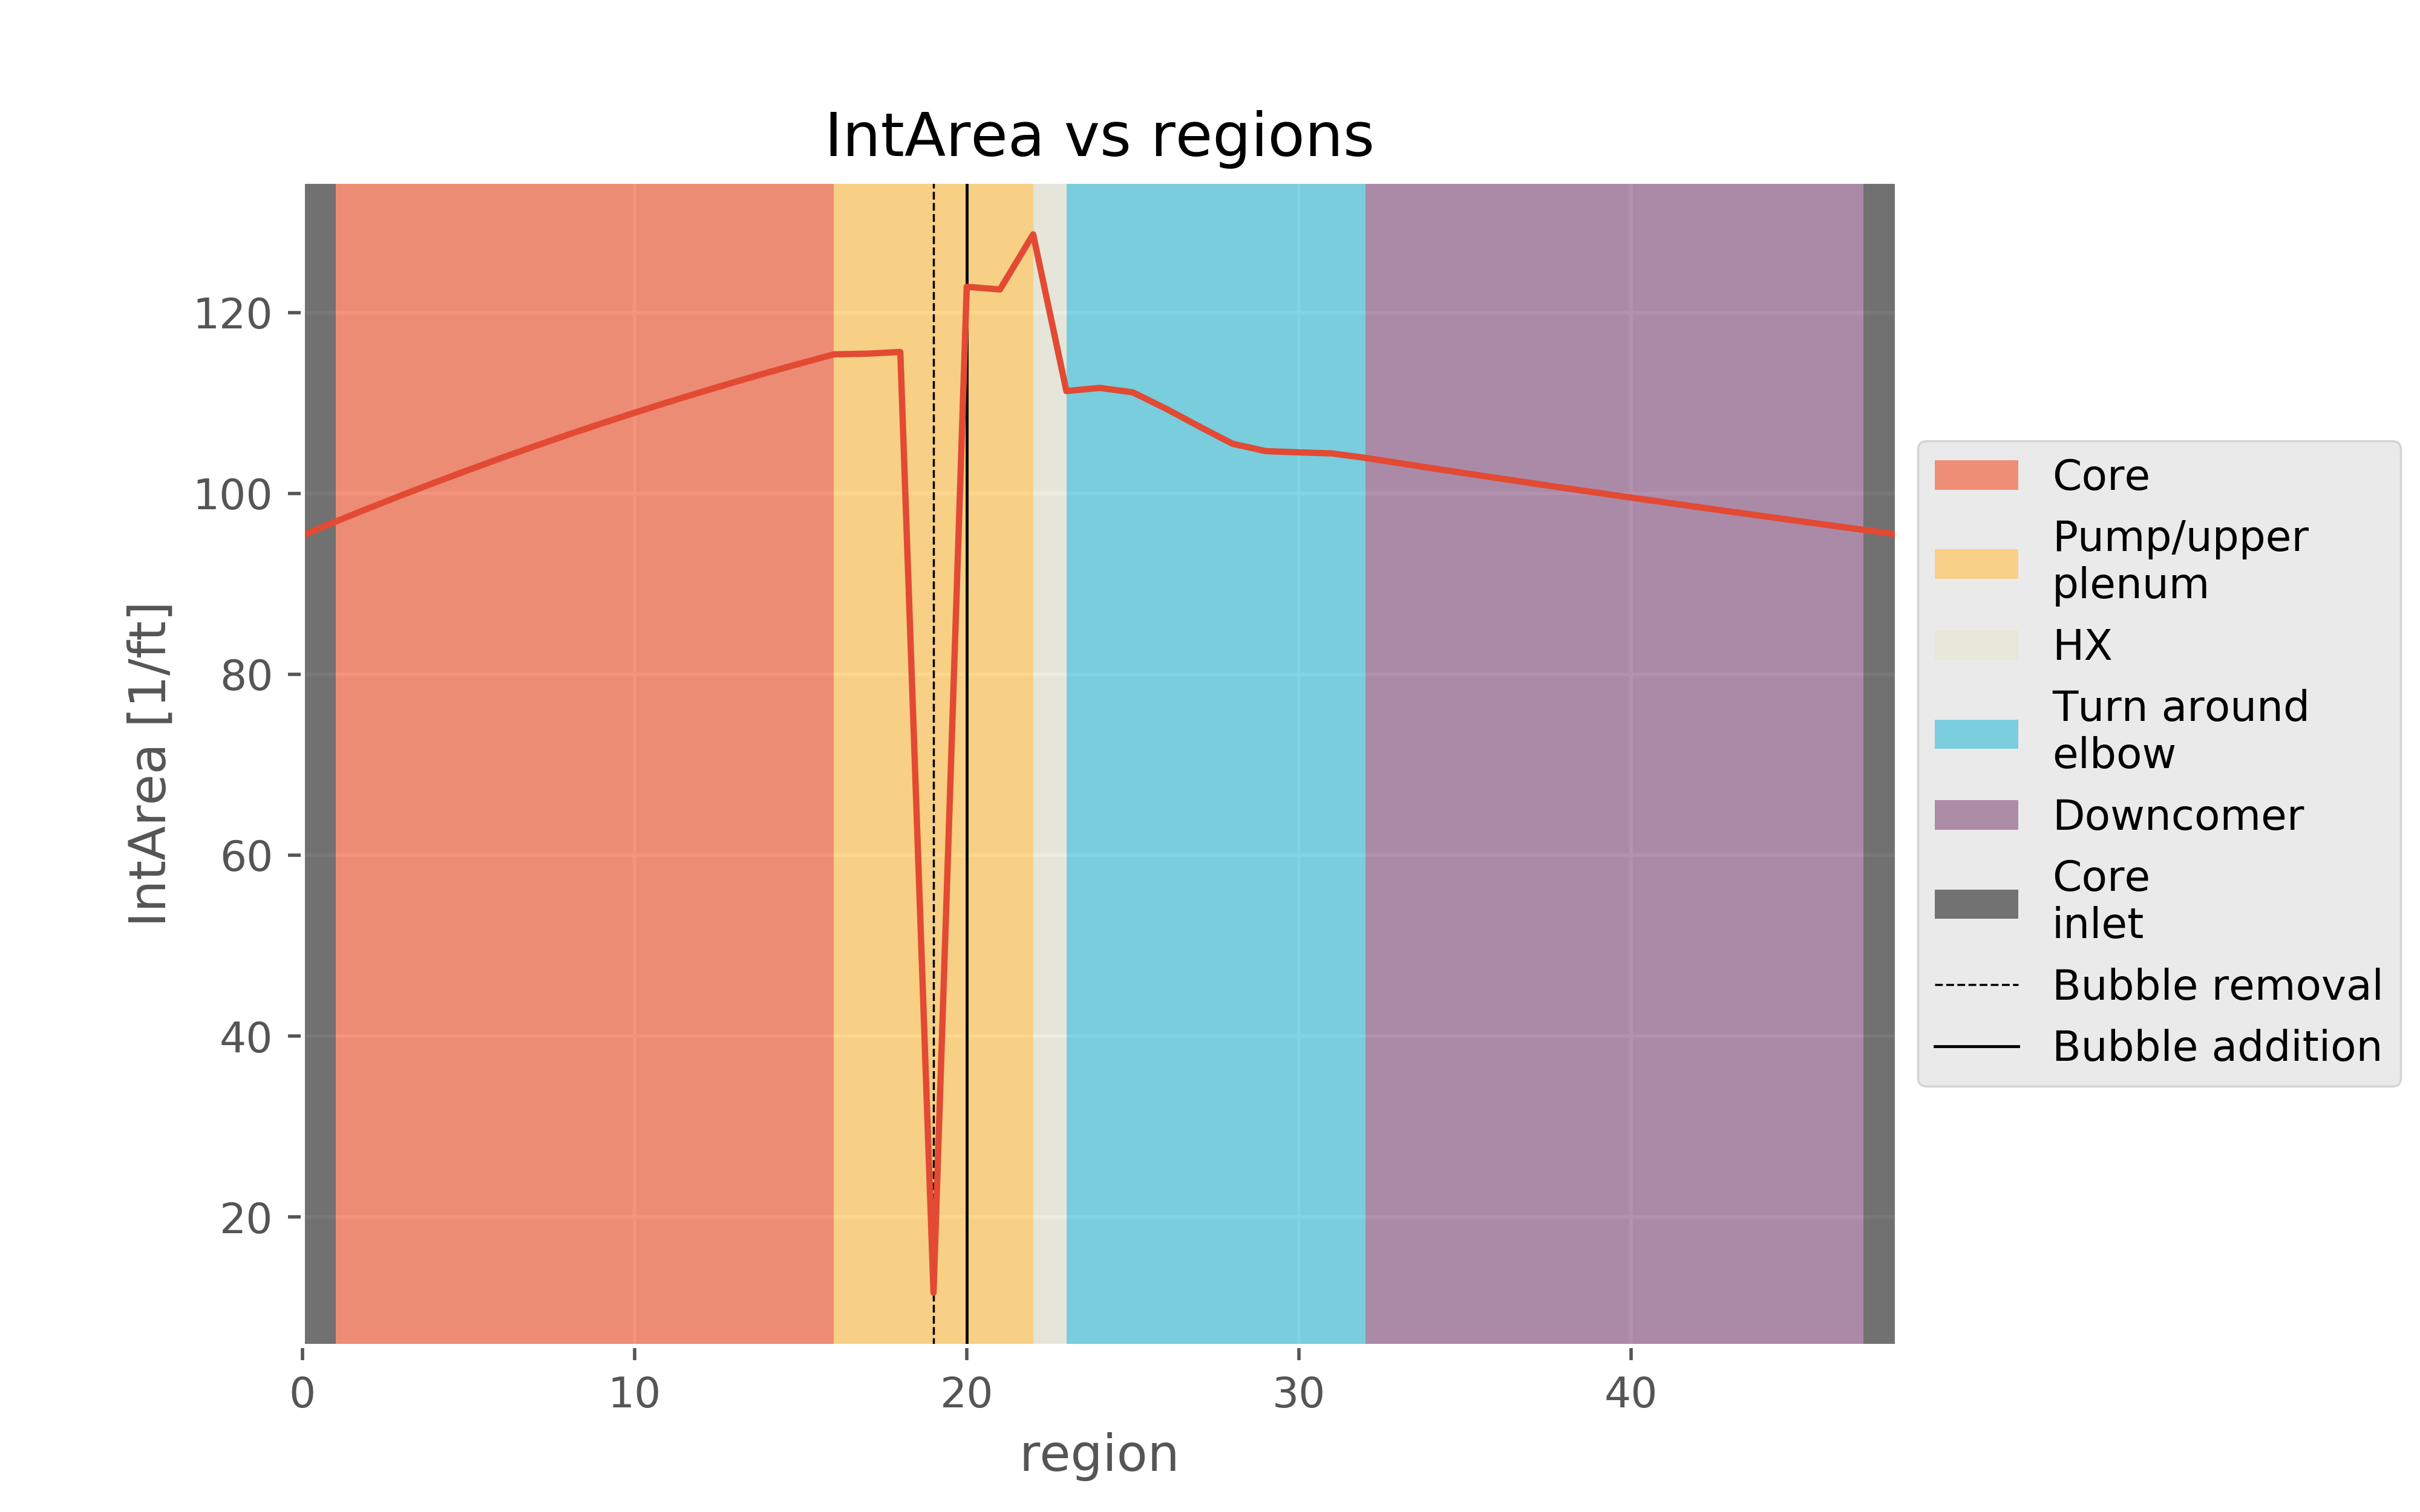
\includegraphics[width=1.0\linewidth]{images/BaseCaseIntArea.png}
  \captionof{figure}{Interfacial area concentration}
  \label{fig:BaseCaseIntAreaCon}
\end{minipage}%
\begin{minipage}{.5\textwidth}
  \centering
  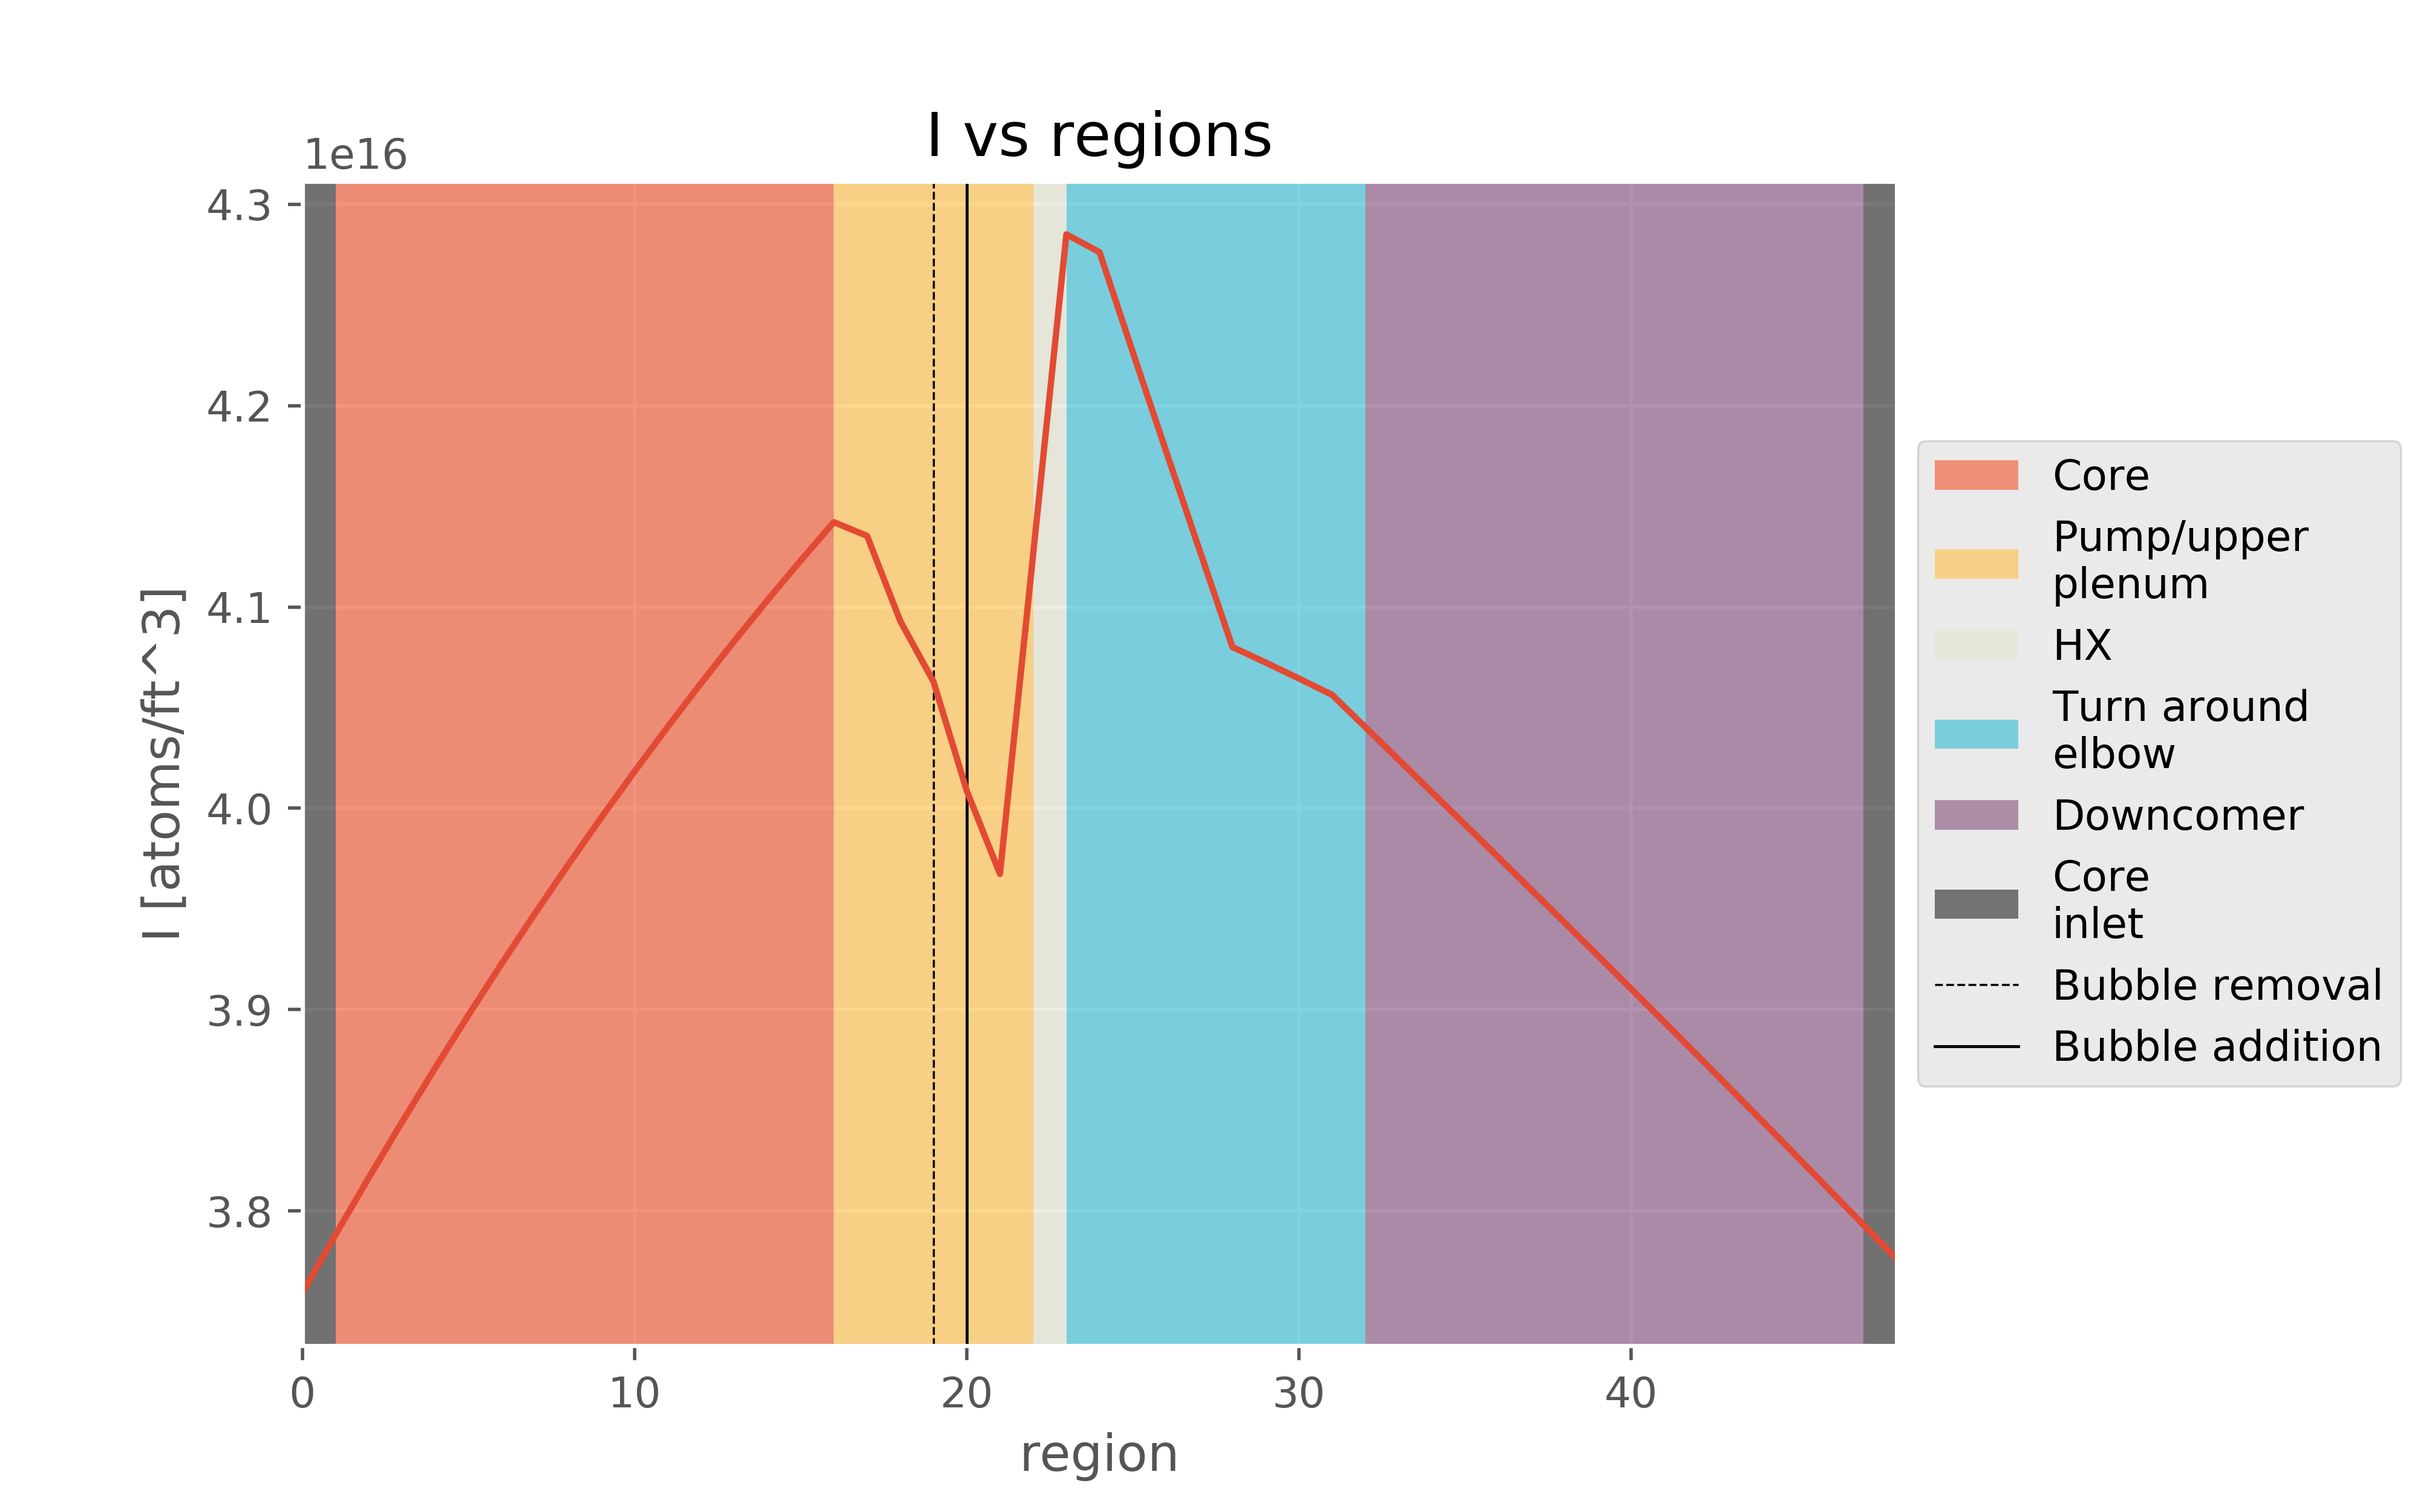
\includegraphics[width=1.0\linewidth]{images/BaseCaseI.png}
  \captionof{figure}{Iodine dissolve in the liquid}
  \label{fig:BaseCaseI}
\end{minipage}
\end{figure}

% HeLiq and HeGas
\begin{figure}[ht] 
\centering
\begin{minipage}{.5\textwidth}
  \centering
  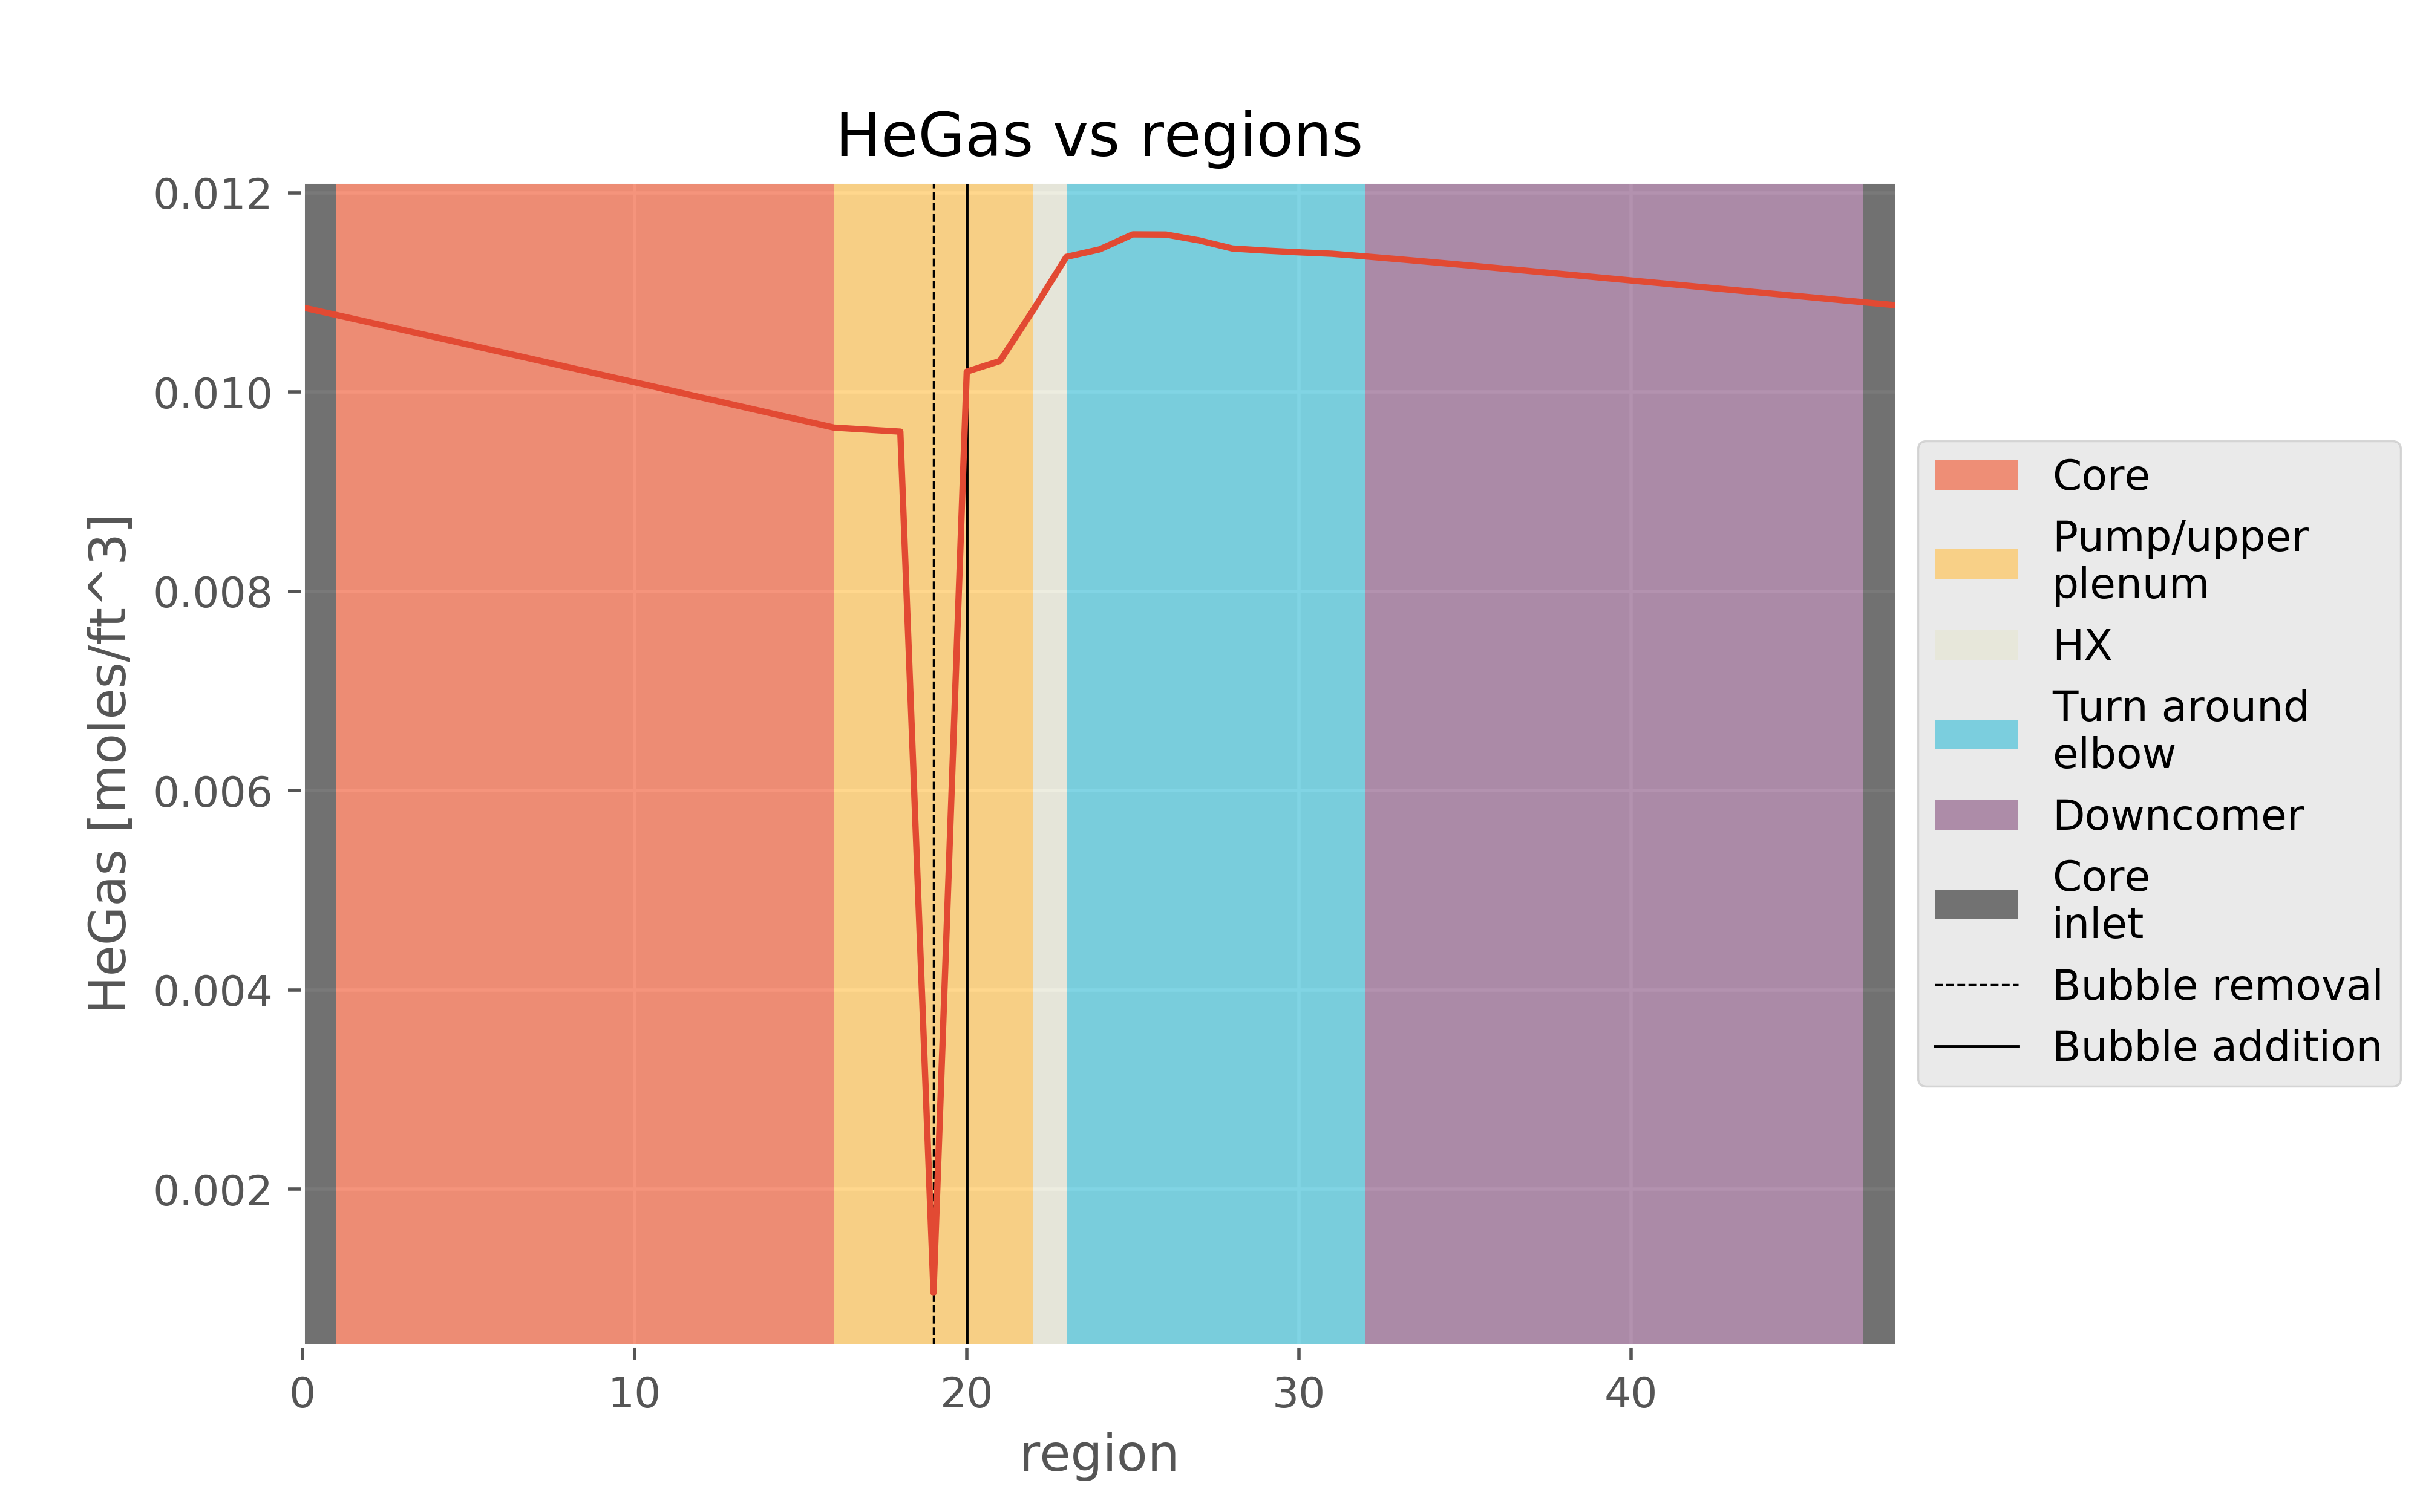
\includegraphics[width=1.0\linewidth]{images/BaseCaseHeGas.png}
  \captionof{figure}{Helium in bubbles}
  \label{fig:BaseCaseHeGas}
\end{minipage}%
\begin{minipage}{.5\textwidth}
  \centering
  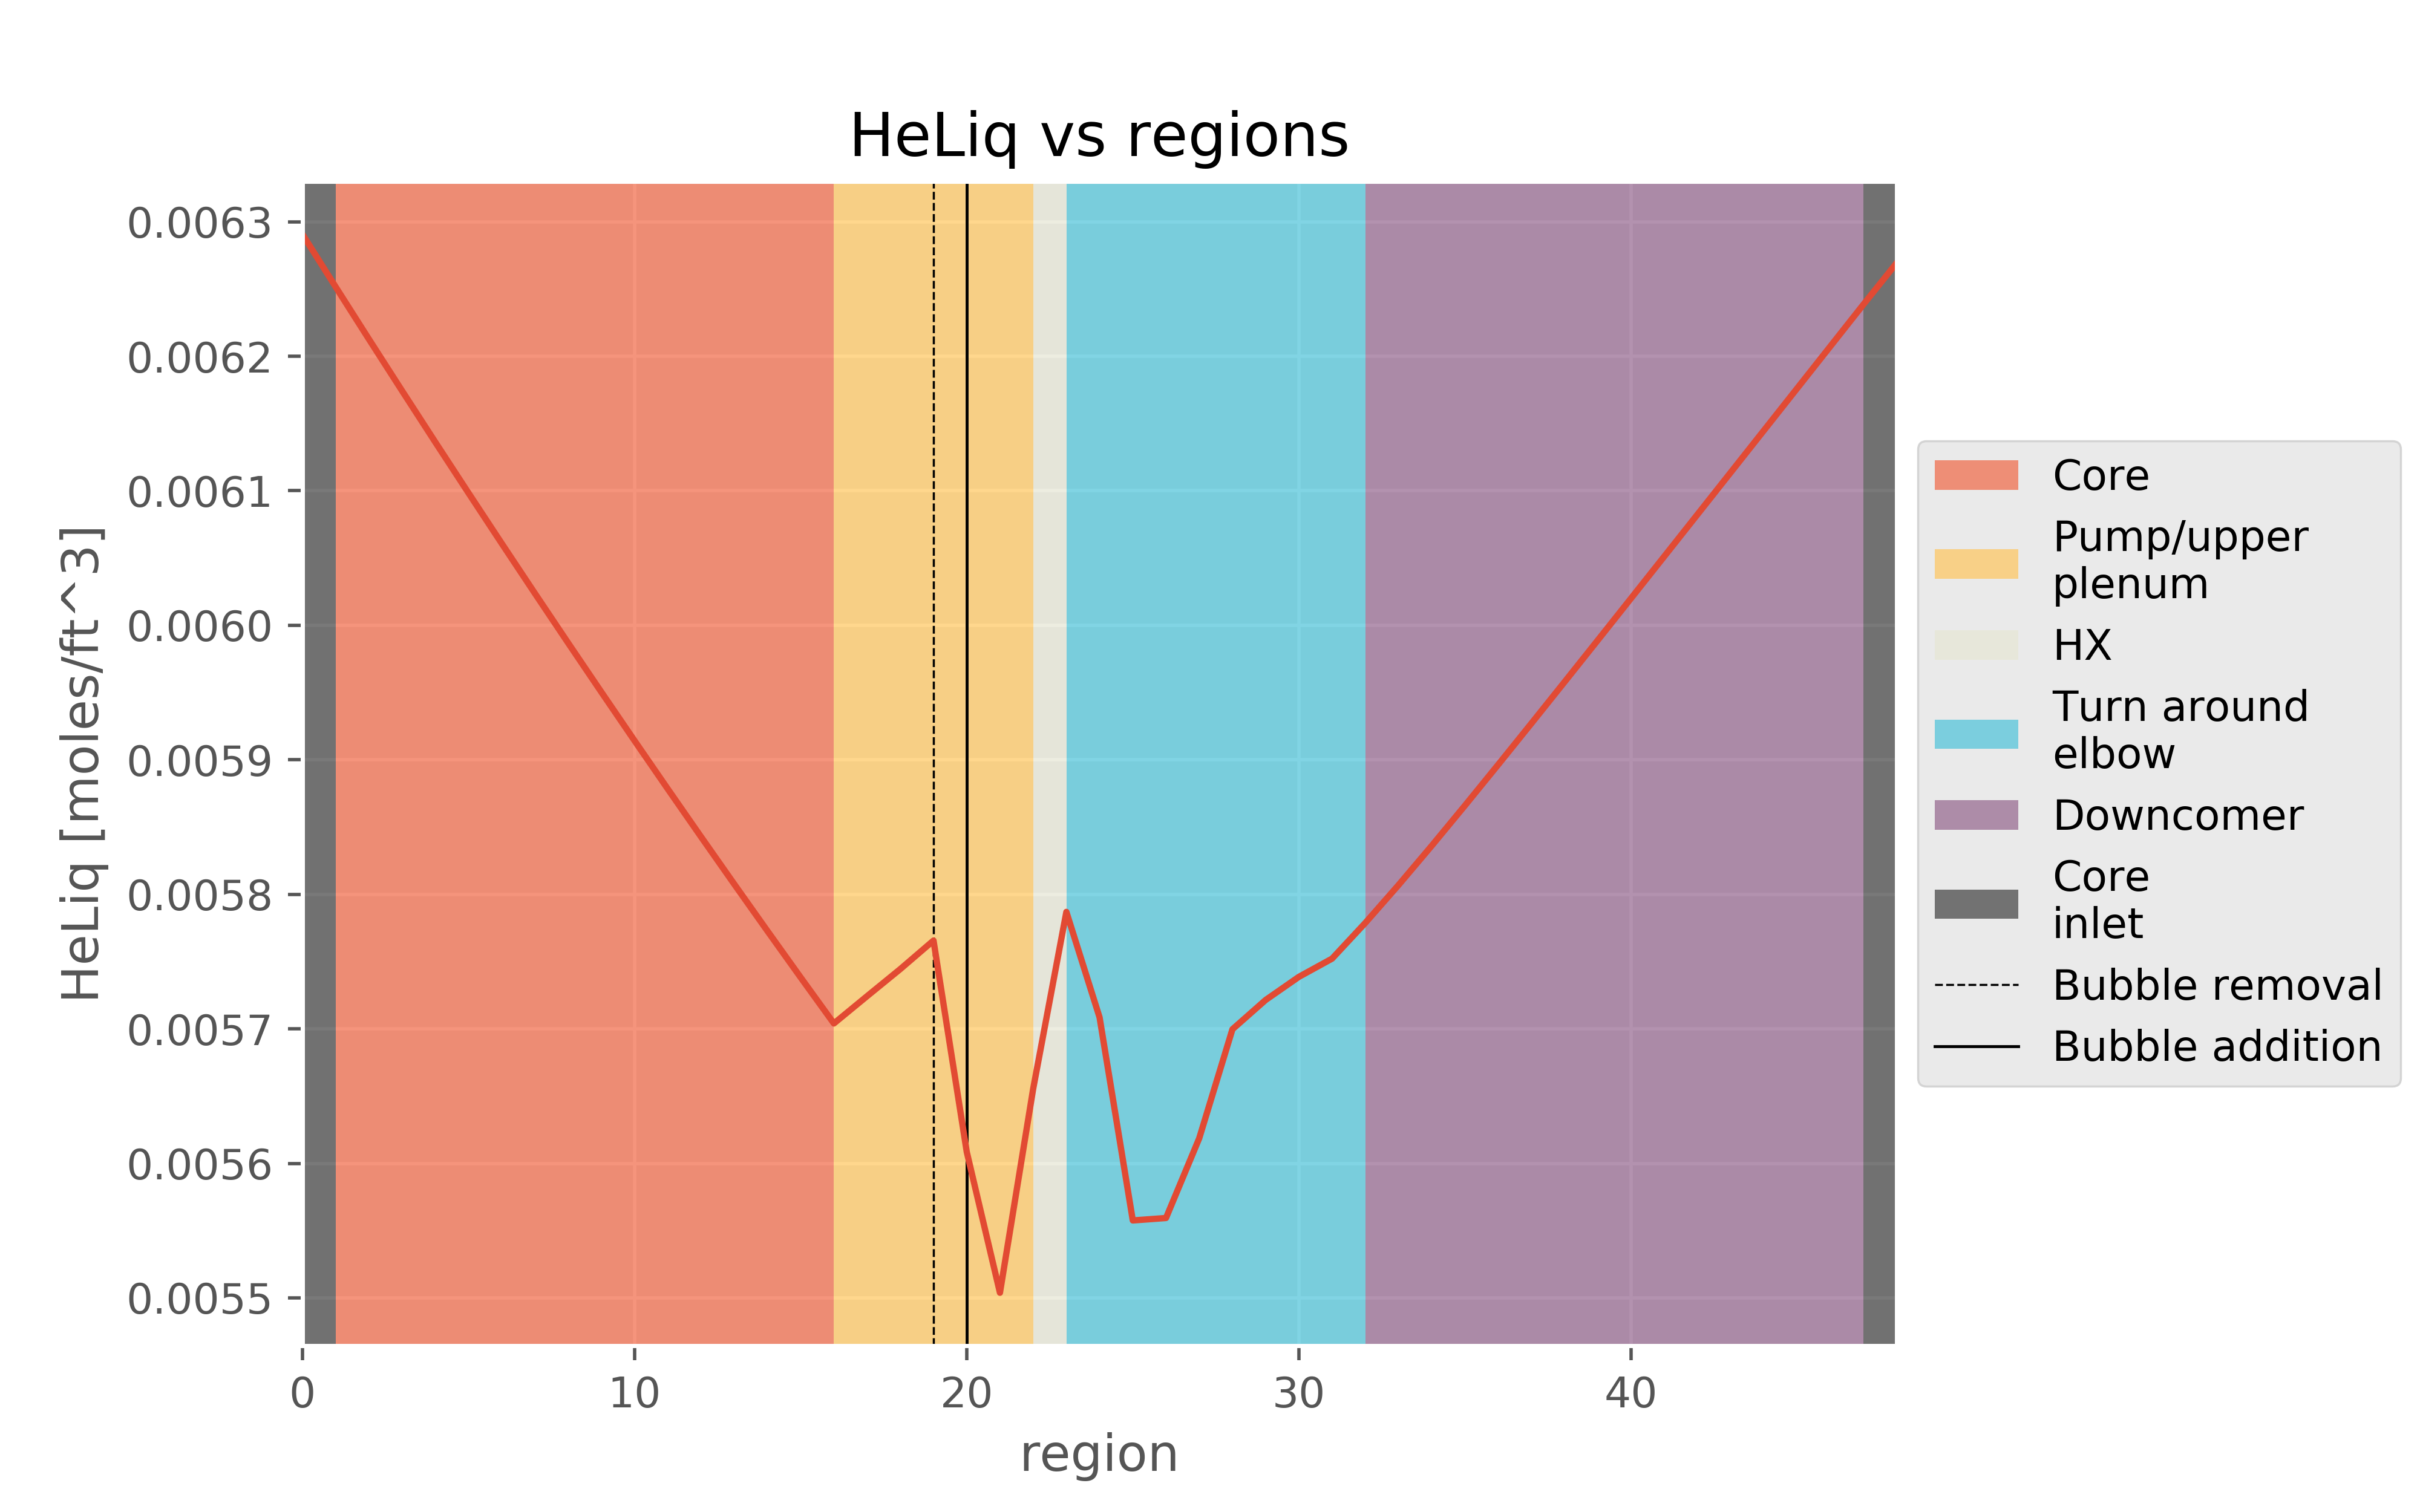
\includegraphics[width=1.0\linewidth]{images/BaseCaseHeLiq.png}
  \captionof{figure}{Helium in the liquid}
  \label{fig:BaseCaseHeLiq}
\end{minipage}
\end{figure}

% XeLiq XeGas 
\begin{figure}[ht] 
\centering
\begin{minipage}{.5\textwidth}
  \centering
  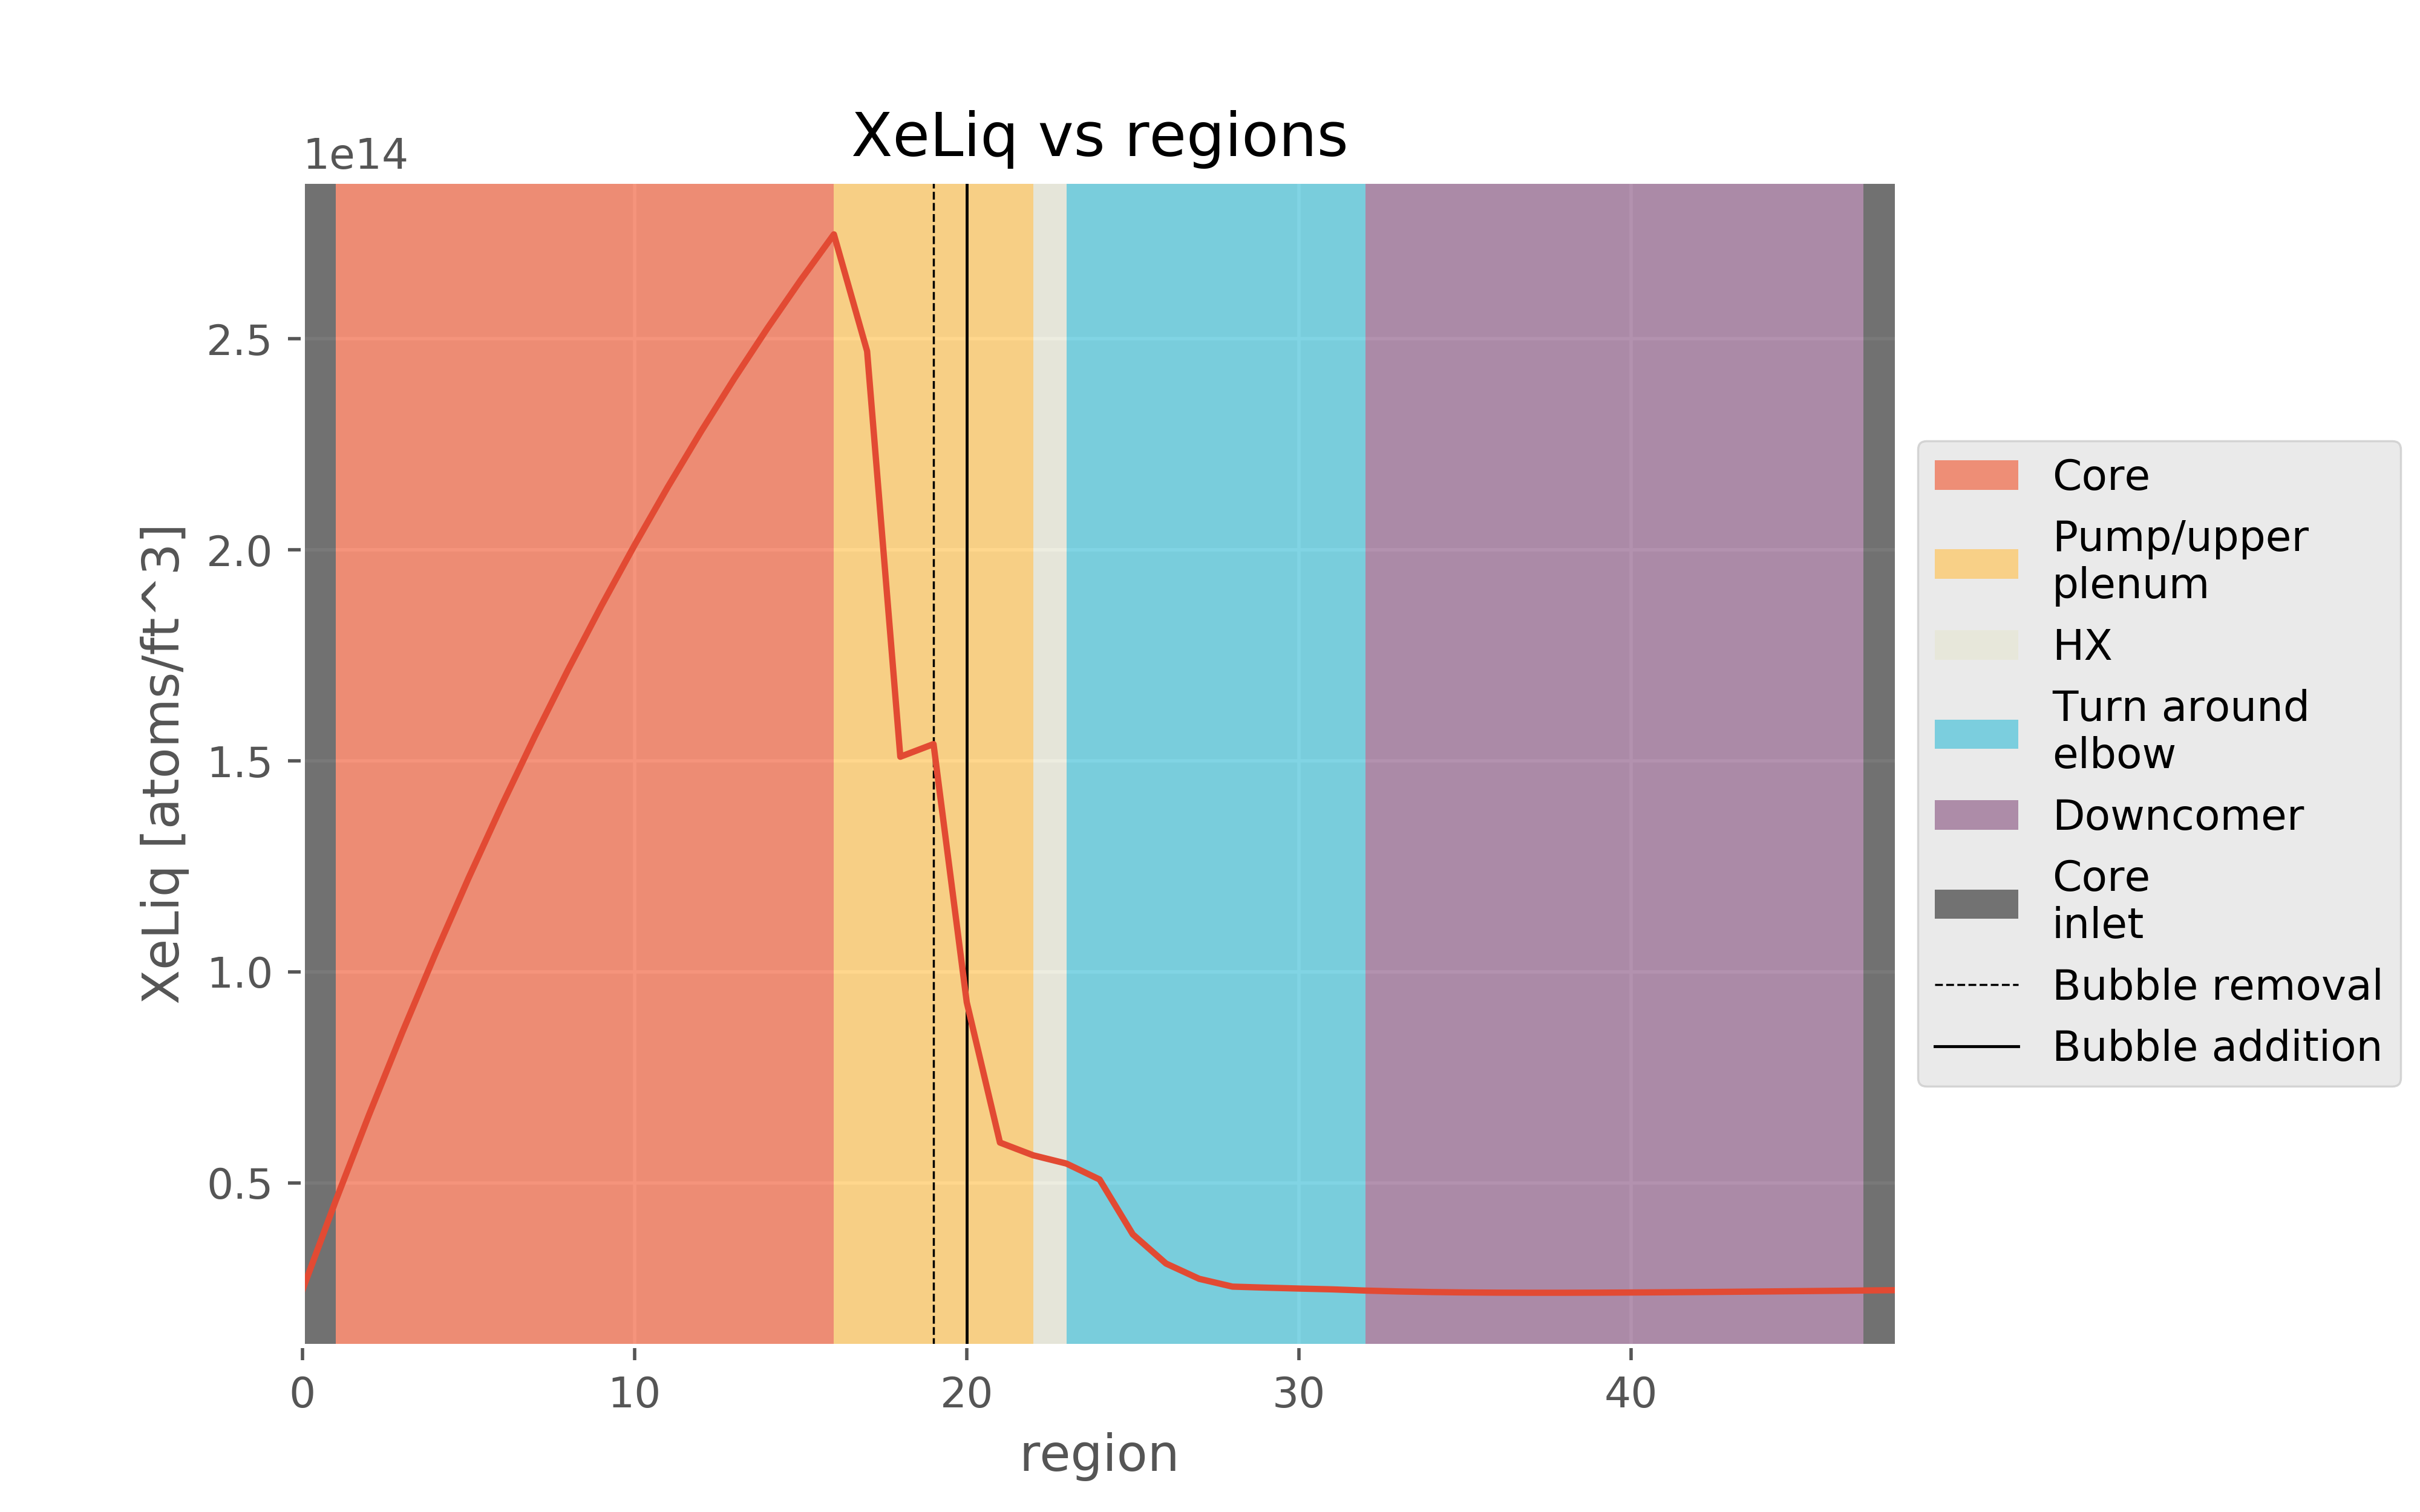
\includegraphics[width=1.0\linewidth]{images/BaseCaseXeLiq.png}
  \captionof{figure}{Xenon in the liquid}
  \label{fig:BaseCaseXeLiq}
\end{minipage}%
\begin{minipage}{.5\textwidth}
  \centering
  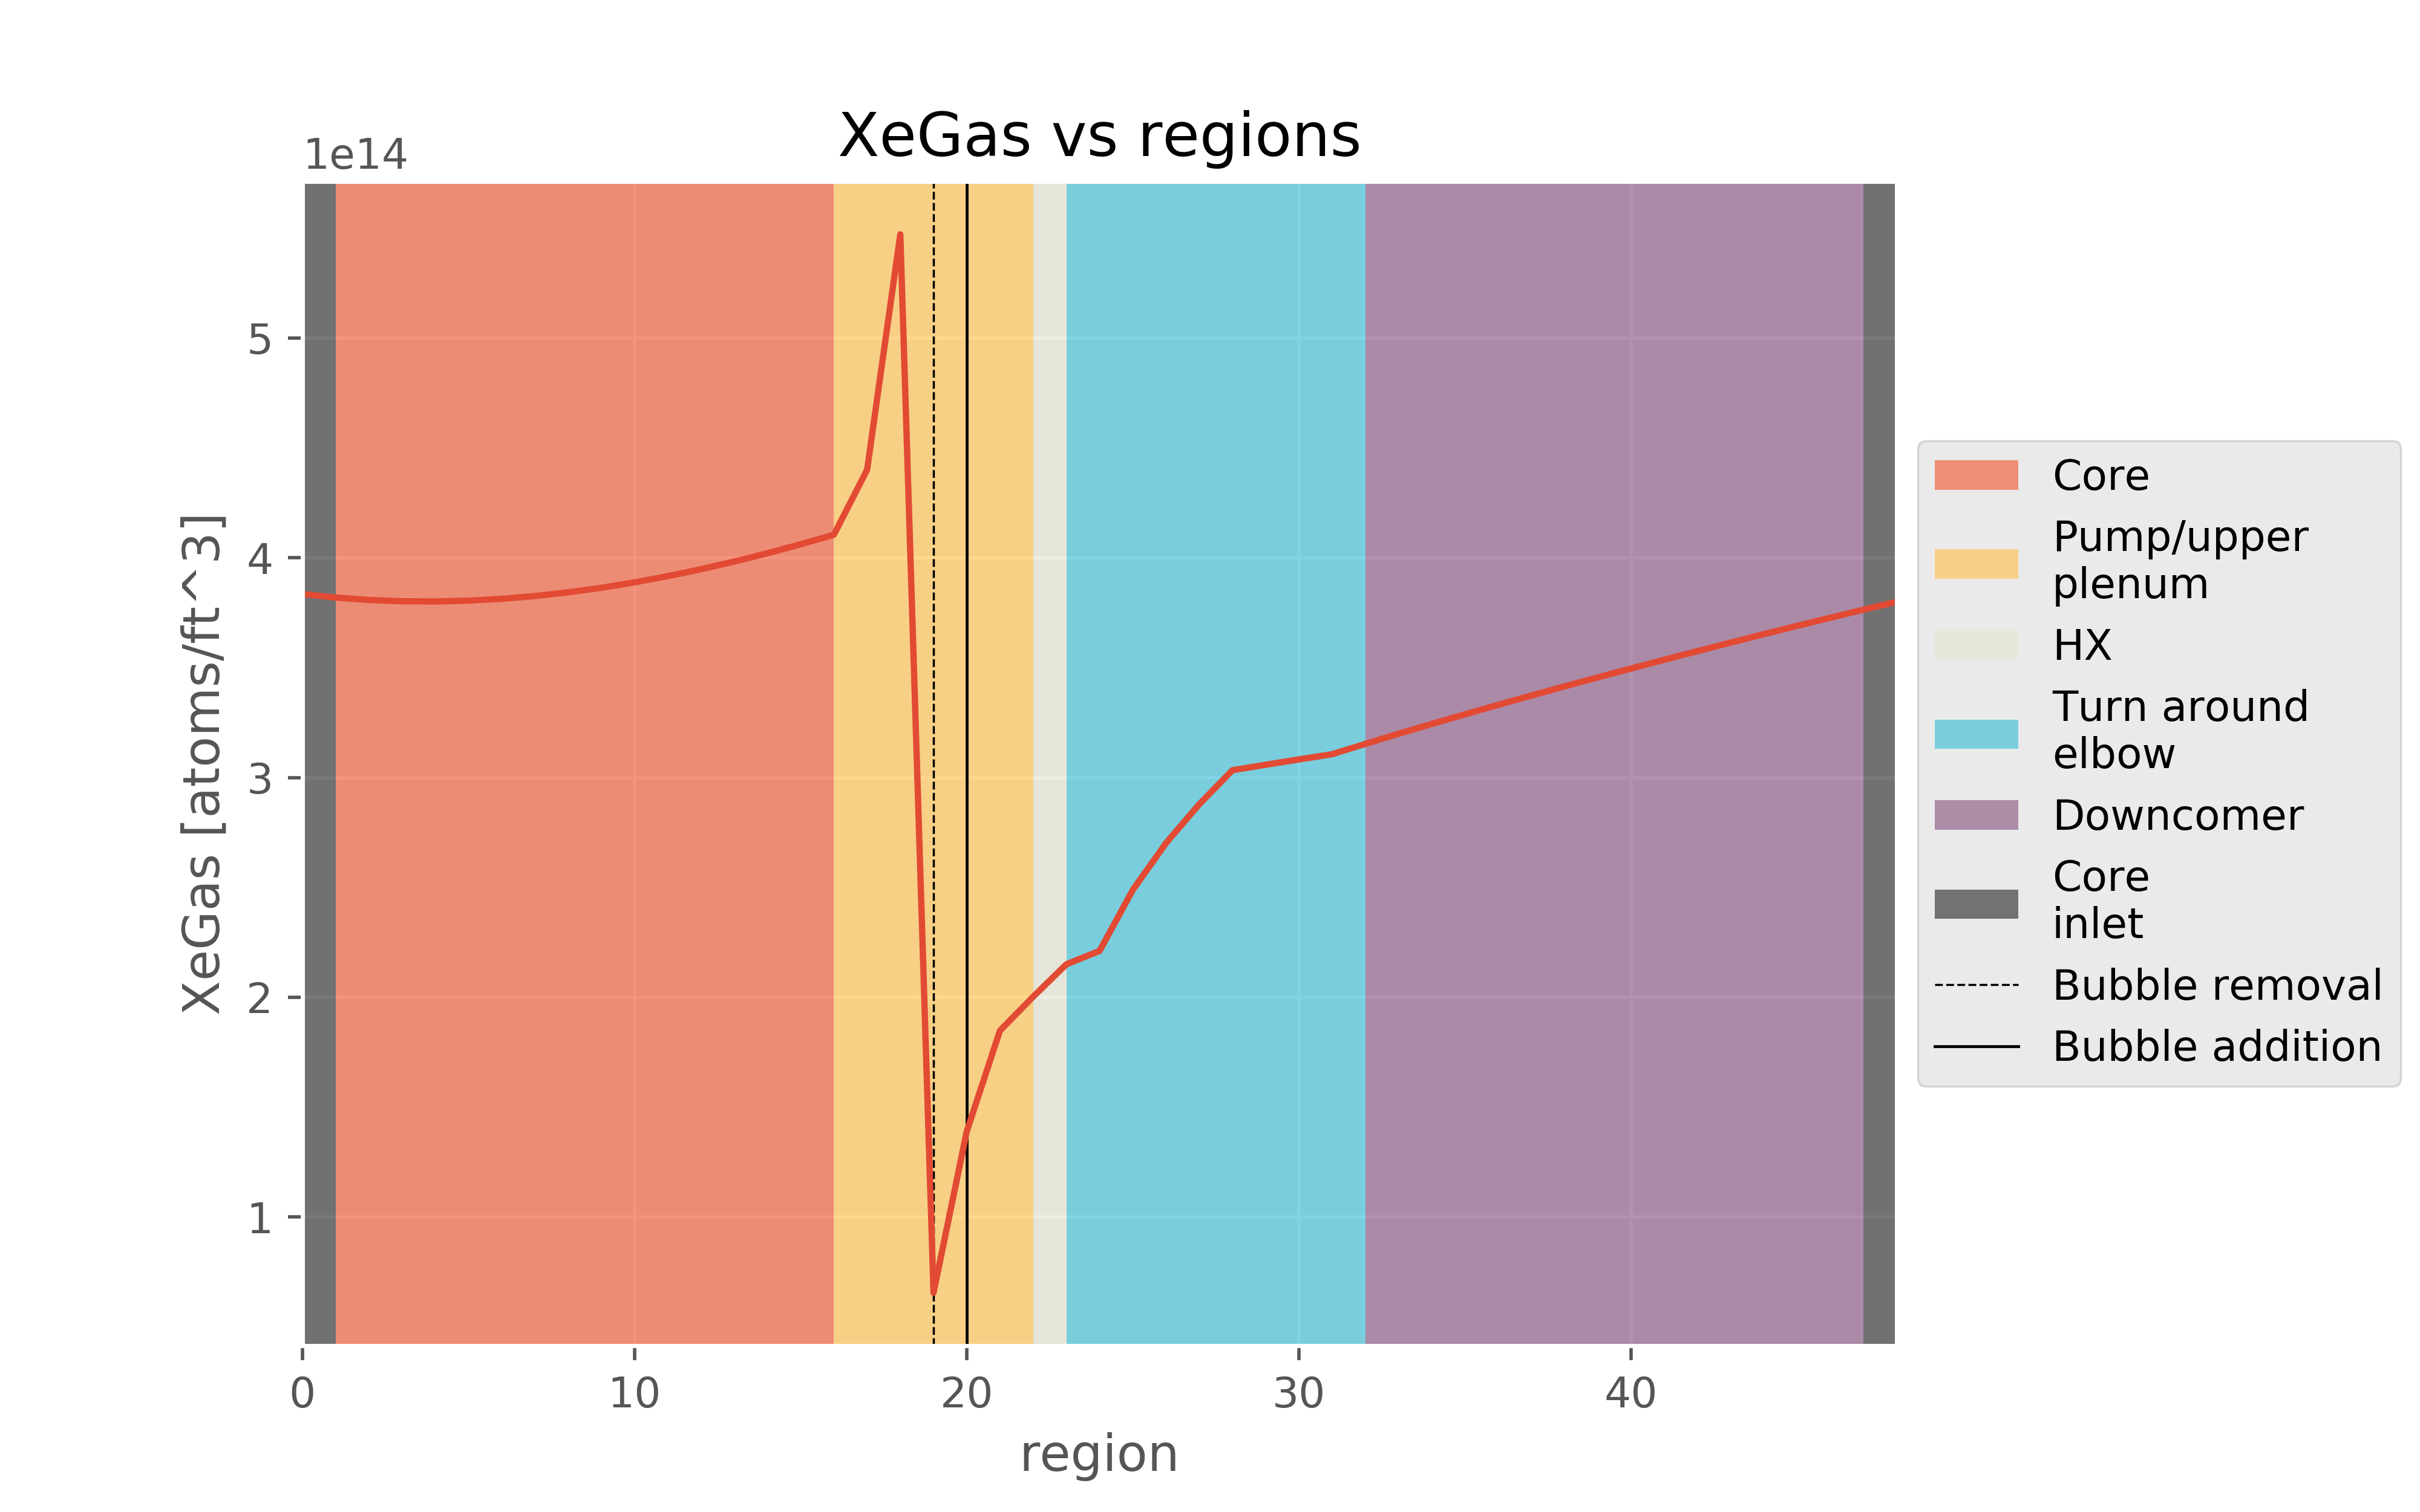
\includegraphics[width=1.0\linewidth]{images/BaseCaseXeGas.png}
  \captionof{figure}{Xenon in the bubbles}
  \label{fig:BaseCaseXeGas}
\end{minipage}
\end{figure}

% percent xe
\begin{figure}[ht]
  \centering
  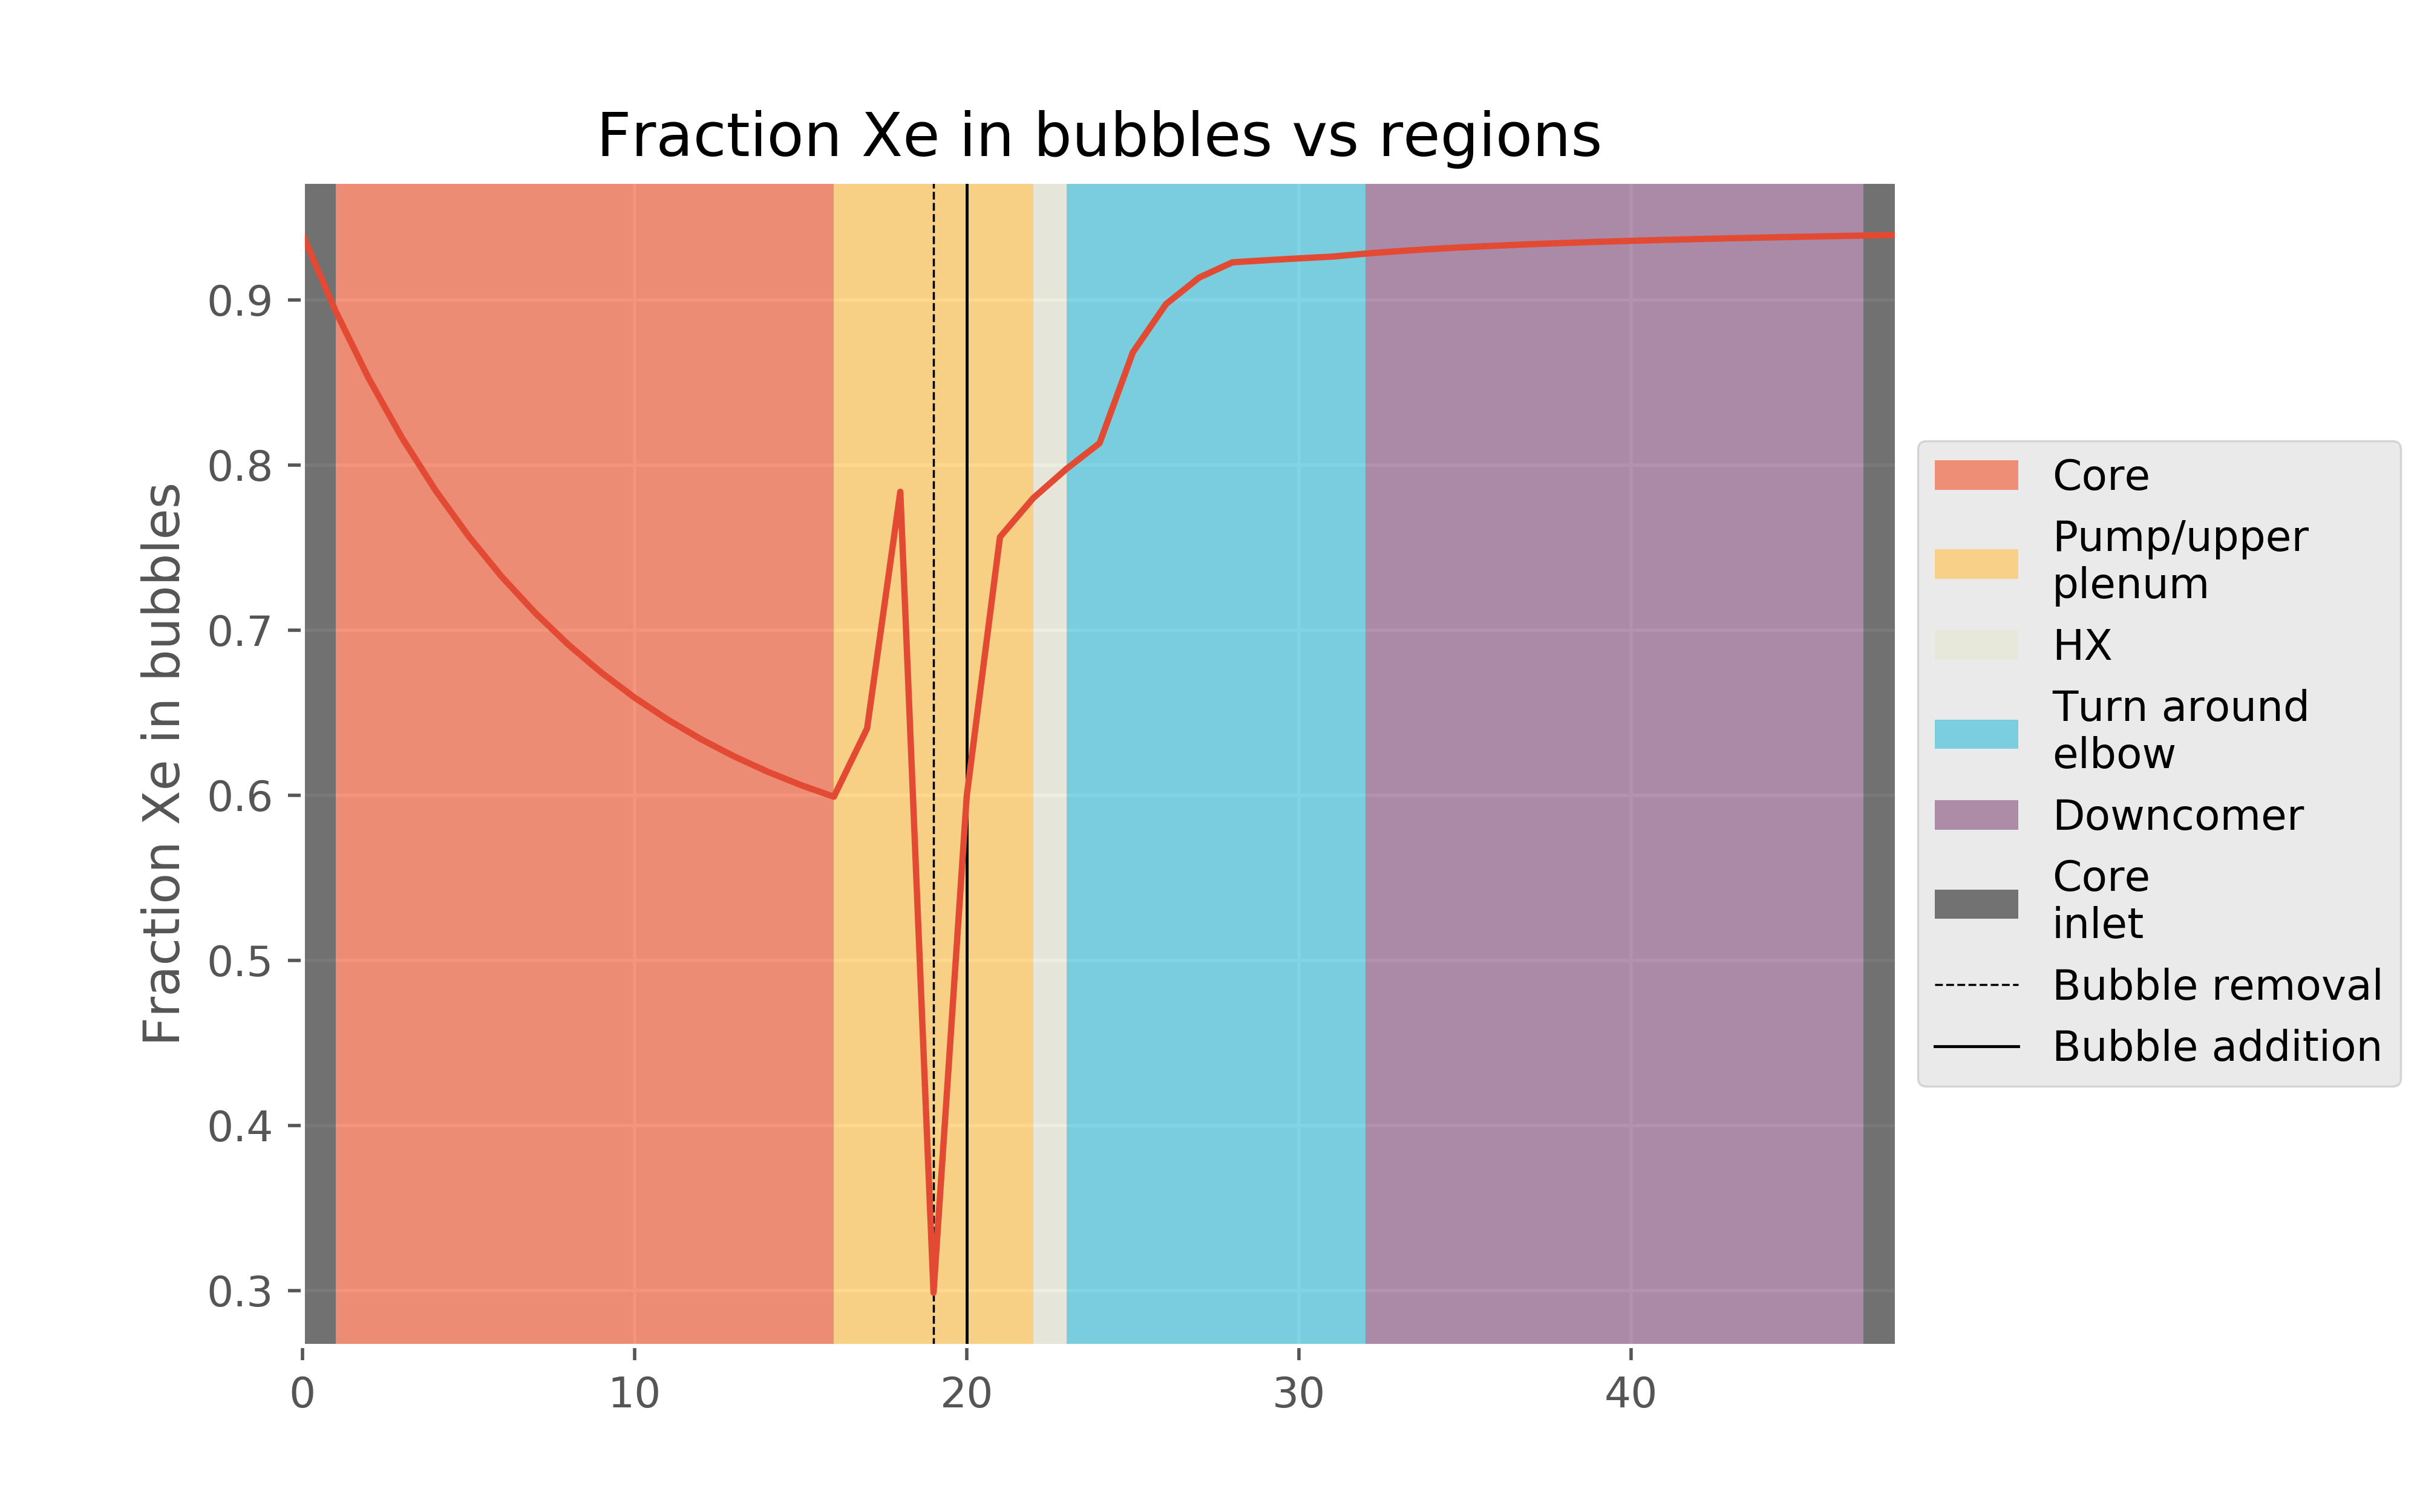
\includegraphics[width=3.5in]{images/BaseCaseFractionXeInBubbles.png}\\
  \caption{Fraction of xenon in bubbles}
  \label{fig:BaseCaseXePercent}
\end{figure}

\FloatBarrier

Interfacial area, bubble diameter and void fractions all follow the same trends. In Figures \ref{fig:BaseCaseDia}, \ref{fig:BaseCaseVoid} and \ref{fig:BaseCaseIntAreaCon} all three variables show an increase in the core region. The core experiences a temperature increase and a pressure decrease, both which contribute to the increase. There is also an increase from mass transfer of the xenon dissolved in the liquid to the bubbles. Void fraction and interfacial area concentration show sharp decreases at the bubble removal location and increases at the bubble injection point. After the pump, diameter, void and interfacial area drop along the heat exchanger, which is attributed to the decrease in temperature. After the heat exchanger a notable drop in pressure is experienced, leading to drops in bubble diameter, void and interfacial area concentration. 

Shown in Figure \ref{fig:BaseCaseI}, iodine increases while traveling up the reactor core as the core is the only generation source. Once above the core, iodine ceases to be generated and begins to decay into xenon for the remainder of the loop. The only exception to this increase in the jump across the heat exchanger. This jump is attributed to the decrease in fluid density as heat is taken away. A reduction in fluid density causes the fluid to slow down, showing an increase in iodine concentration. 

Helium dissolved in the liquid, shown in Figure \ref{fig:BaseCaseHeLiq}, seems to trend with the velocity distribution. This is the same reason the iodine concentration increases across the heat exchanger. As helium travels up the core, the density decreases causing an increase in fluid velocity. This action makes it apparent that the helium concentration is lowering up the core. Three spiked regions occur to the dissolved helium as in travels through the pump, heat exchanger and down comer.  The first spike is an increase after the reactor core. This spike might be attributed to the fact that I am only plotting the on of the core channels and not all four. Once out of the core all channels combine into one which could increase the concentration. The second spike shoots the concentration down after the bubble injection location. A third spike is seen across the heat exchanger, this has been previously discussed. The four spike is right after the heat exchanger. It is unknown why the second and fourth spikes occur. After the fourth spike, the concentration increases in the down comer. This increase is caused by mass transfer from the helium bubbles to the liquid. Helium in the bubbles, shown in Figure \ref{fig:BaseCaseHeGas}, follows a similar, slight decrease across the core. Attributed to both mass transfer and velocity increases. At the bubble removal location a reduction in concentration is seen because the bubbles are removed. The following spike is from gas being injected into the system.

Xenon dissolved in the liquid, shown in Figure \ref{fig:BaseCaseXeLiq}, is generated in the liquid as the fluid passes through the core. After the core it seems that is decay term overpowers the fluctuations in concentration from changes in fluid density. As the dissolved xenon travels through the pump, turn around and down comer it only decreases in concentration. This decrease is both due to mass transfer into the bubbles and decay of xenon. Xenon trapped in the bubbles, shown in Figure \ref{fig:BaseCaseXeGas}, slightly increase going up the core and experience a large spike right after the core. The spike is likely due to the same reason helium dissolved in the liquid also spiked. At the bubble removal location, a sharp decrease is experienced due to bubble removal. After bubble injection, xenon in the bubbles increases until it loops back into the core. The fraction of xenon, shown in Figure \ref{fig:BaseCaseXePercent} in the bubbles decreases in the core because the rate of xenon generation in the liquid is far greater than the rate of mass transfer into the bubbles. A spike after the core is experience and has been previously discussed. At the removal location a spike is seen, followed by increases due to mass transfer into the bubbles. 

% change in bubble diameter
\subsection{Change in Injected Bubble Diameter}
The injected bubble diameter is both increased and decreased 25\%, 50\% and 75\% to determined its effect on the examined variables. While the injected diameter is changed the overall void should not because the boundary condition setter should adjust the number of injected bubbles. From Figure \ref{fig:InjectedVoid}, the void fraction does slightly change, maybe due to the increase in mass transfer into the gas bubbles. As shown in Figures \ref{fig:InjectedDia} and \ref{fig:InjectedIntAreaCon} changing the injection diameter drastically changes the interfacial area. Decreasing the bubble diameter while maintaining the same void fraction increases the overall interfacial area because more bubbles are being injected. The increase in interfacial area increases the source for phase migration of both xenon and helium. Figures \ref{fig:InjectedXeGas}, \ref{fig:InjectedXeLiq} and \ref{fig:InjectedFractionXeInBubbles} shows that more xenon is in the gas bubbles and less is dissolved in the liquid. From Figures \ref{fig:InjectedHeGas} and \ref{fig:InjectedHeLiq}, the change in injected gas bubble diameter doesn't have a significant change in the amount of helium in bubbles.

% void and diameter
\begin{figure}[p] 
\centering
\begin{minipage}{.5\textwidth}
  \centering
  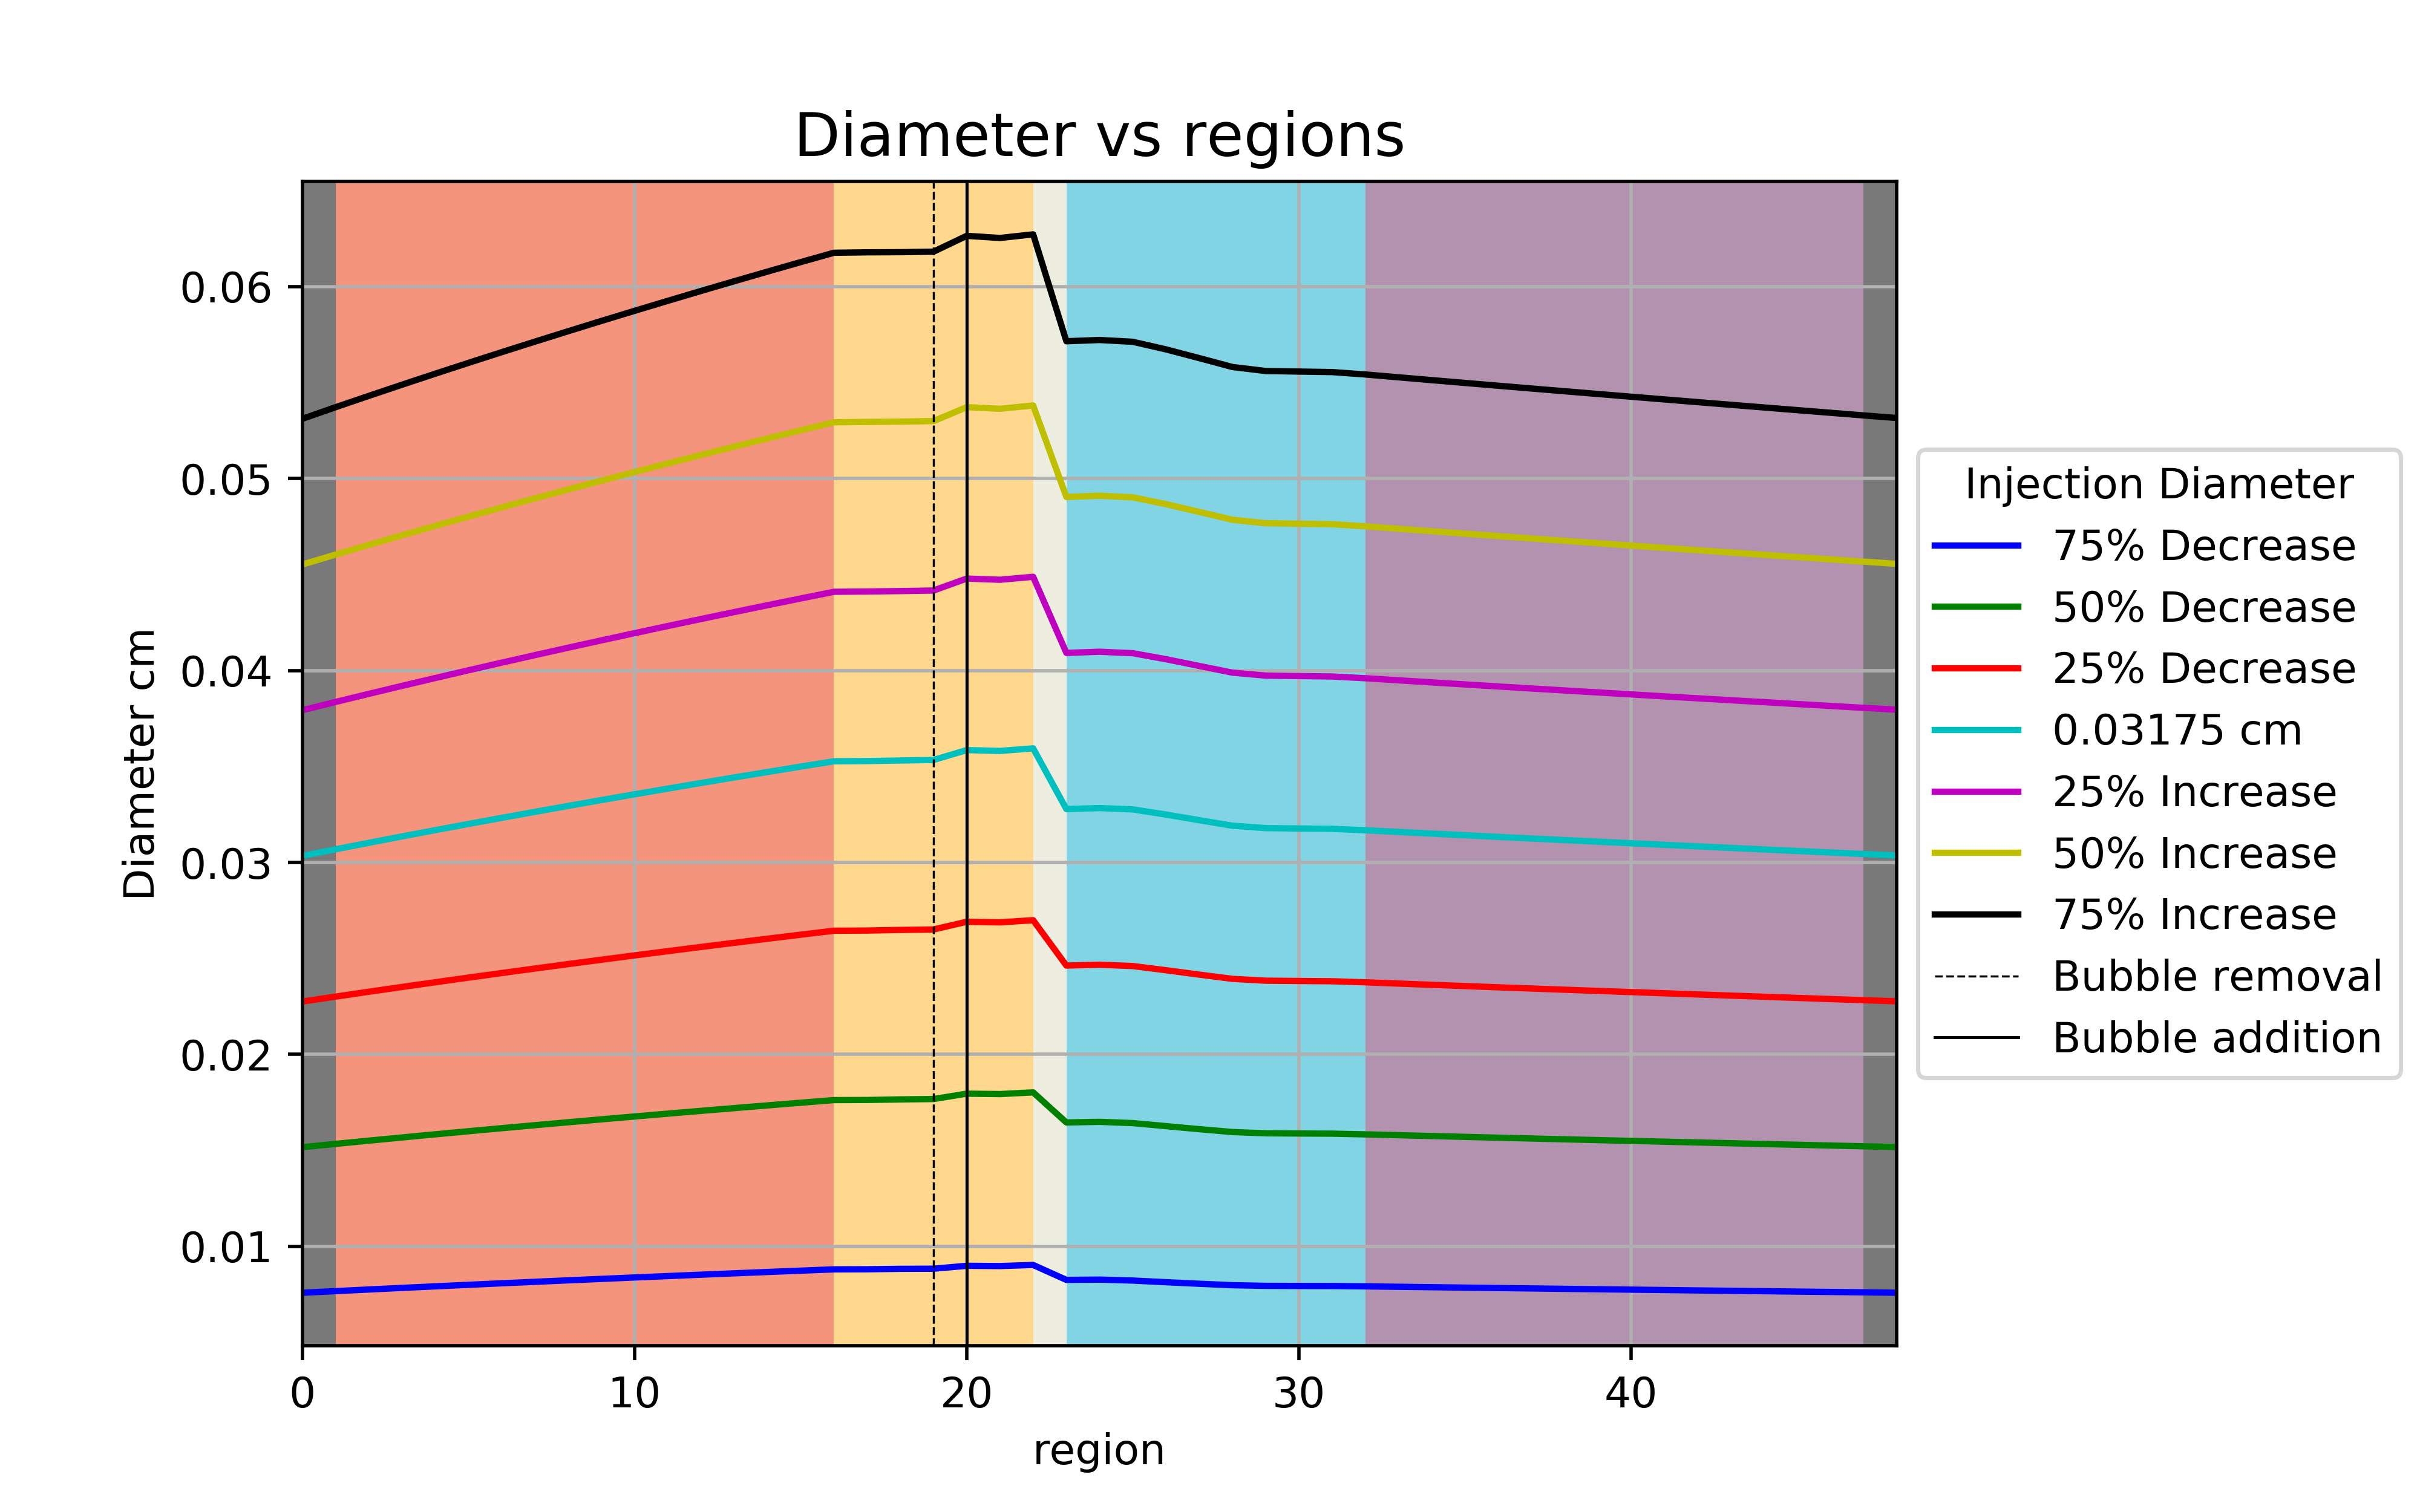
\includegraphics[width=1.0\linewidth]{images/InjectedDiameter.png}
  \captionof{figure}{Changes in bubble diameter \\ with changes in injection diameter}
  \label{fig:InjectedDia}
\end{minipage}%
\begin{minipage}{.5\textwidth}
  \centering
  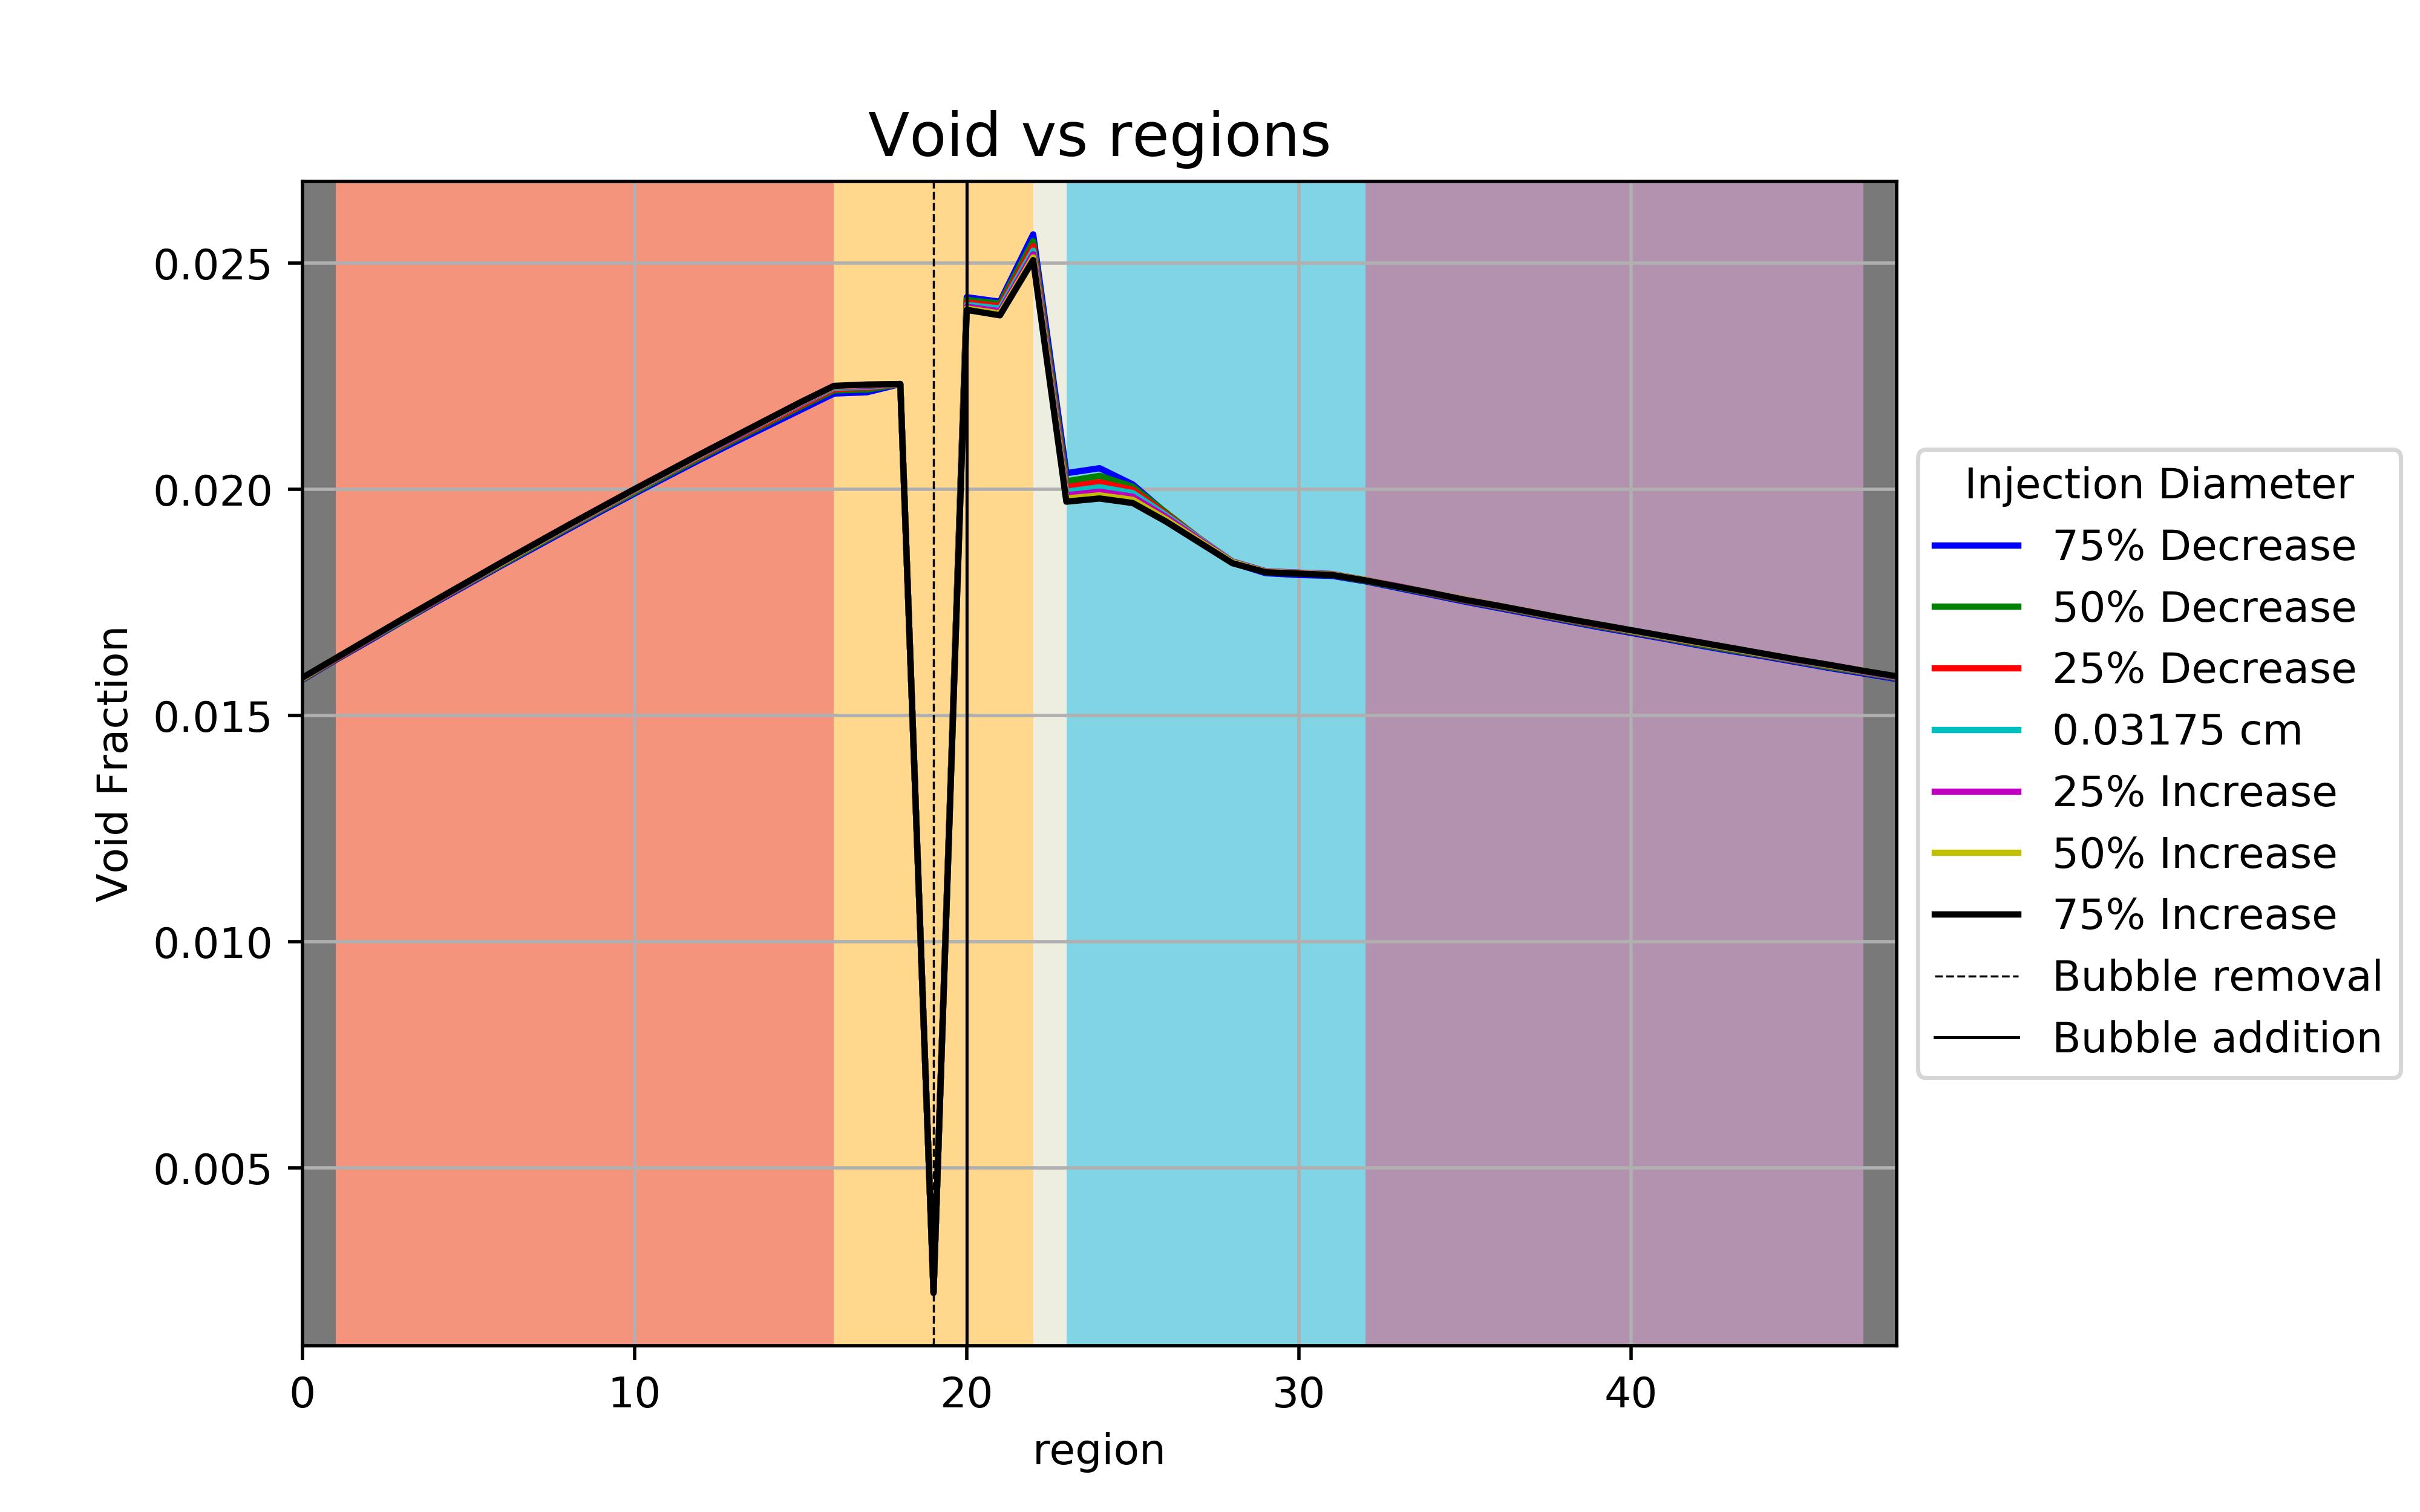
\includegraphics[width=1.0\linewidth]{images/InjectedVoid.png}
  \captionof{figure}{Changes in void fraction \\ with changes in injection diameter}
  \label{fig:InjectedVoid}
\end{minipage}
\end{figure}

% IntArea and Iodine
\begin{figure}[p] 
\centering
\begin{minipage}{.5\textwidth}
  \centering
  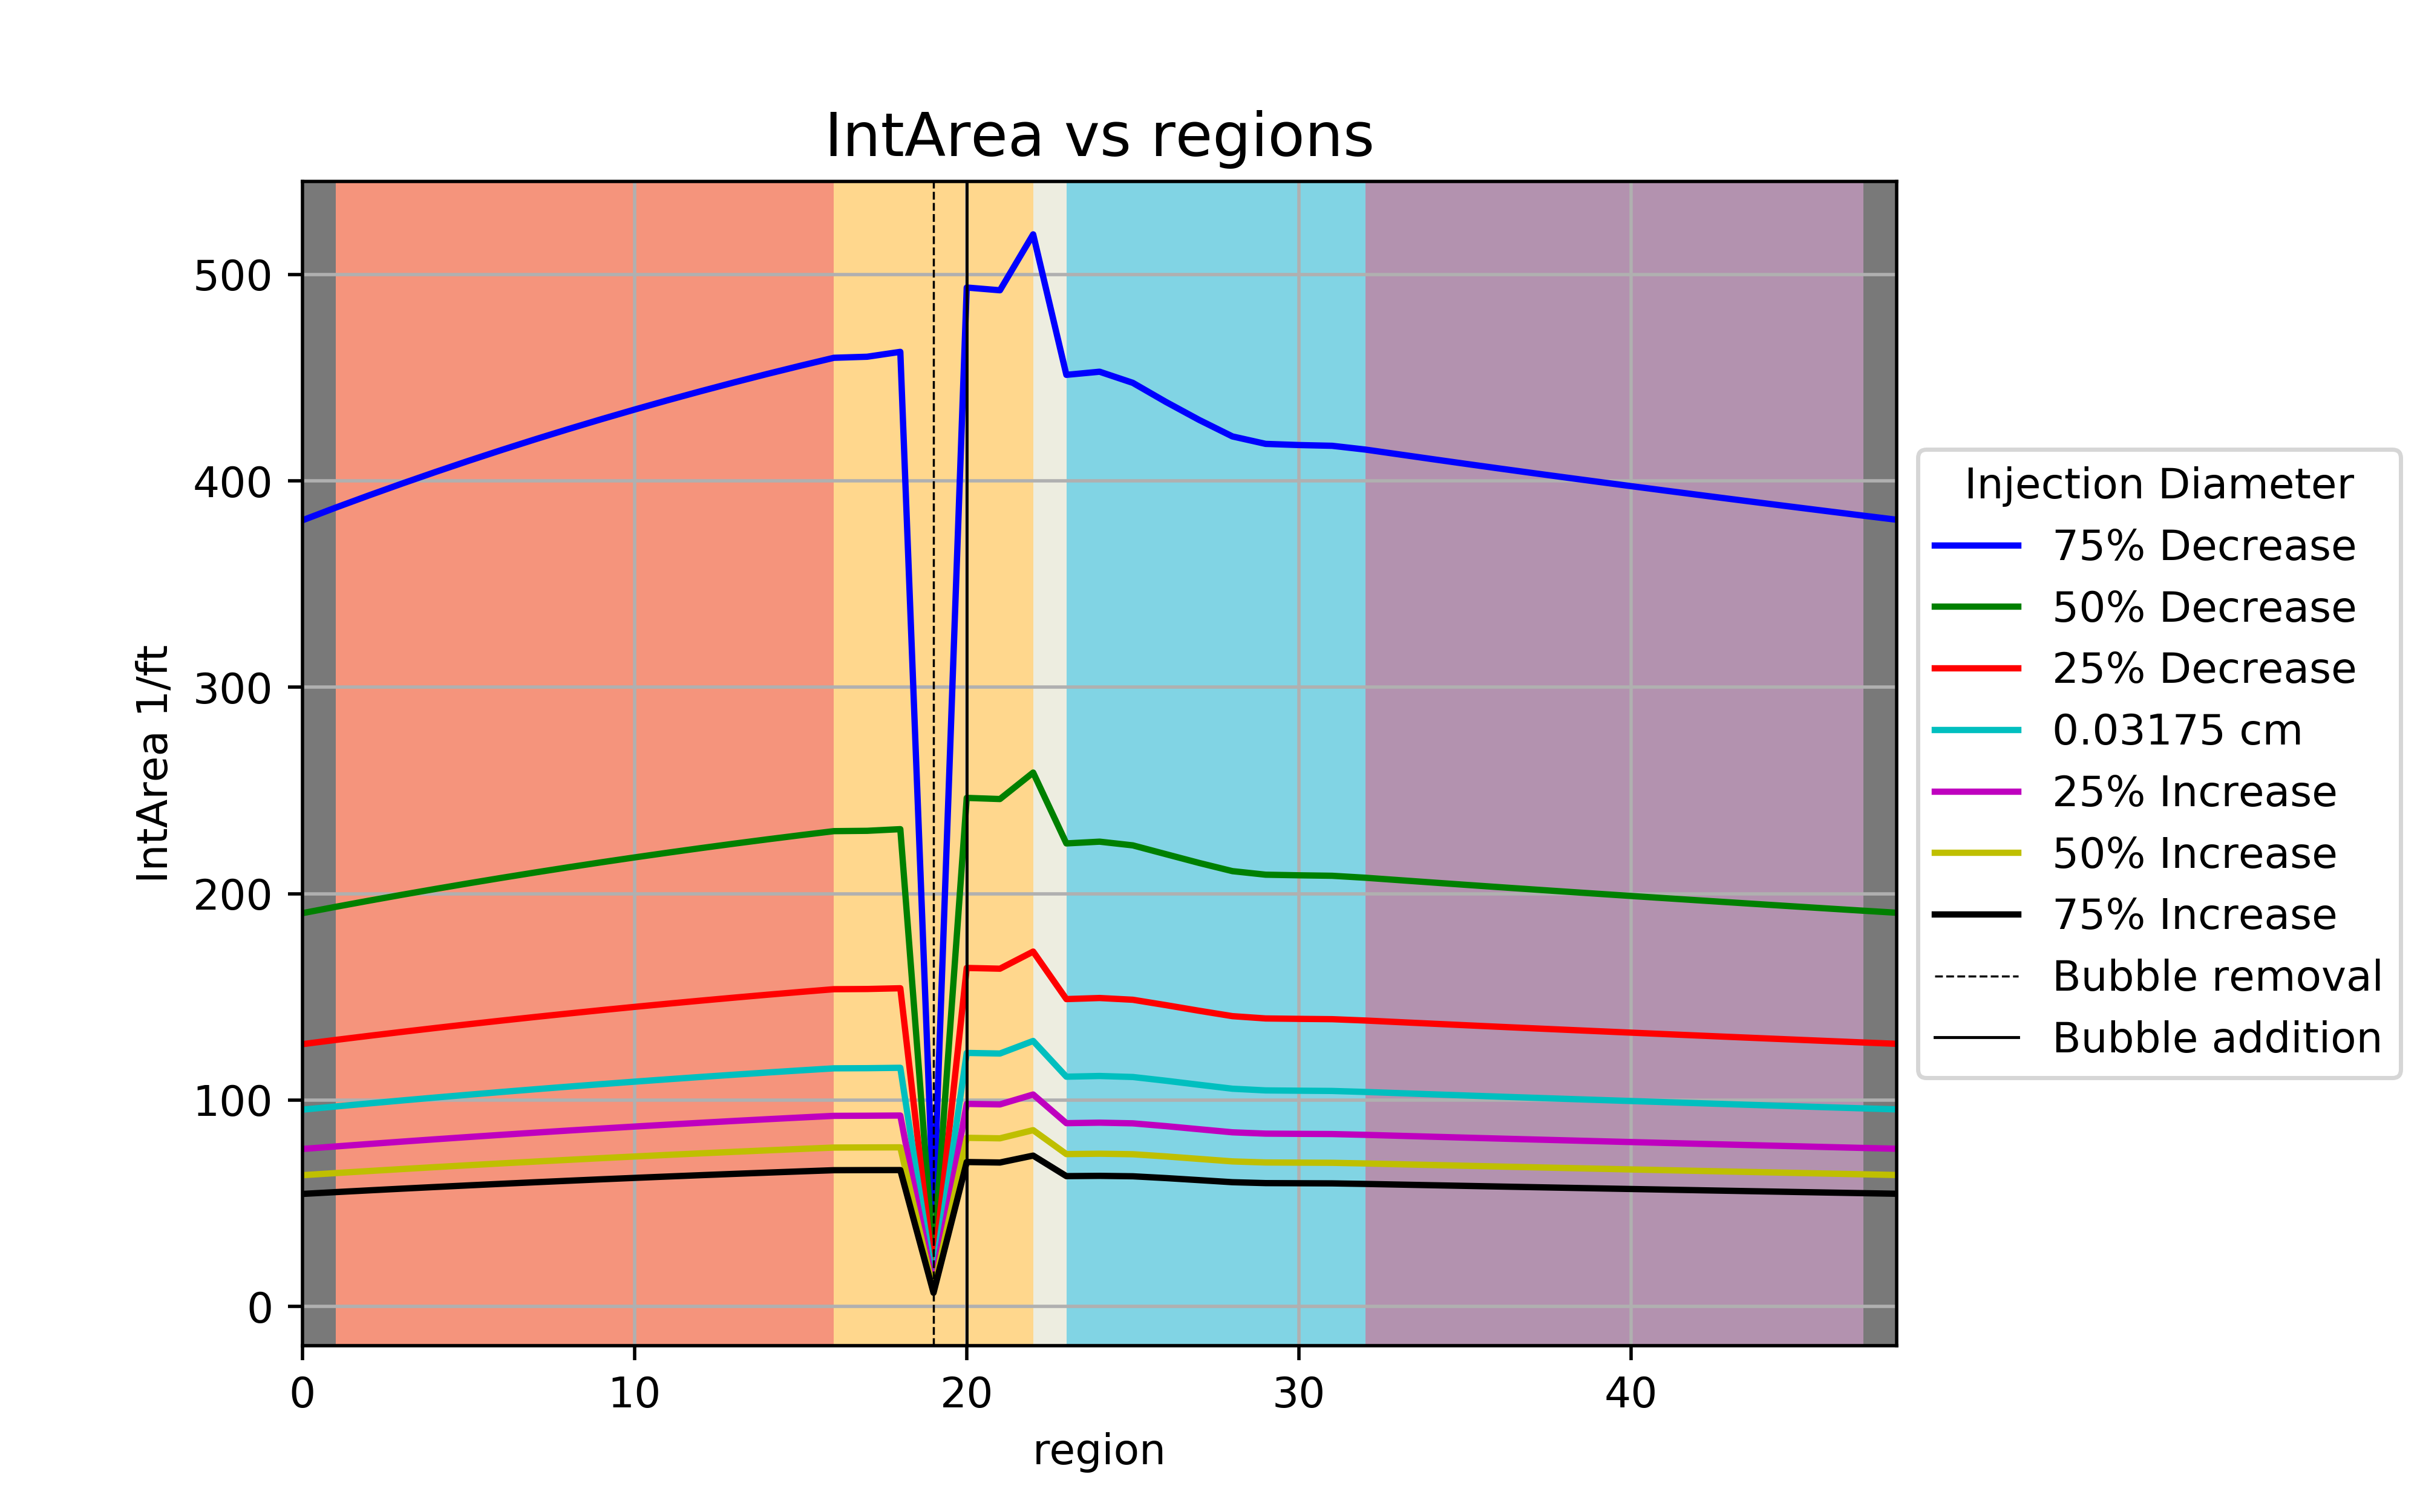
\includegraphics[width=1.0\linewidth]{images/InjectedIntArea.png}
  \captionof{figure}{Changes in interfacial area \\ with changes in injection diameter}
  \label{fig:InjectedIntAreaCon}
\end{minipage}%
\begin{minipage}{.5\textwidth}
  \centering
  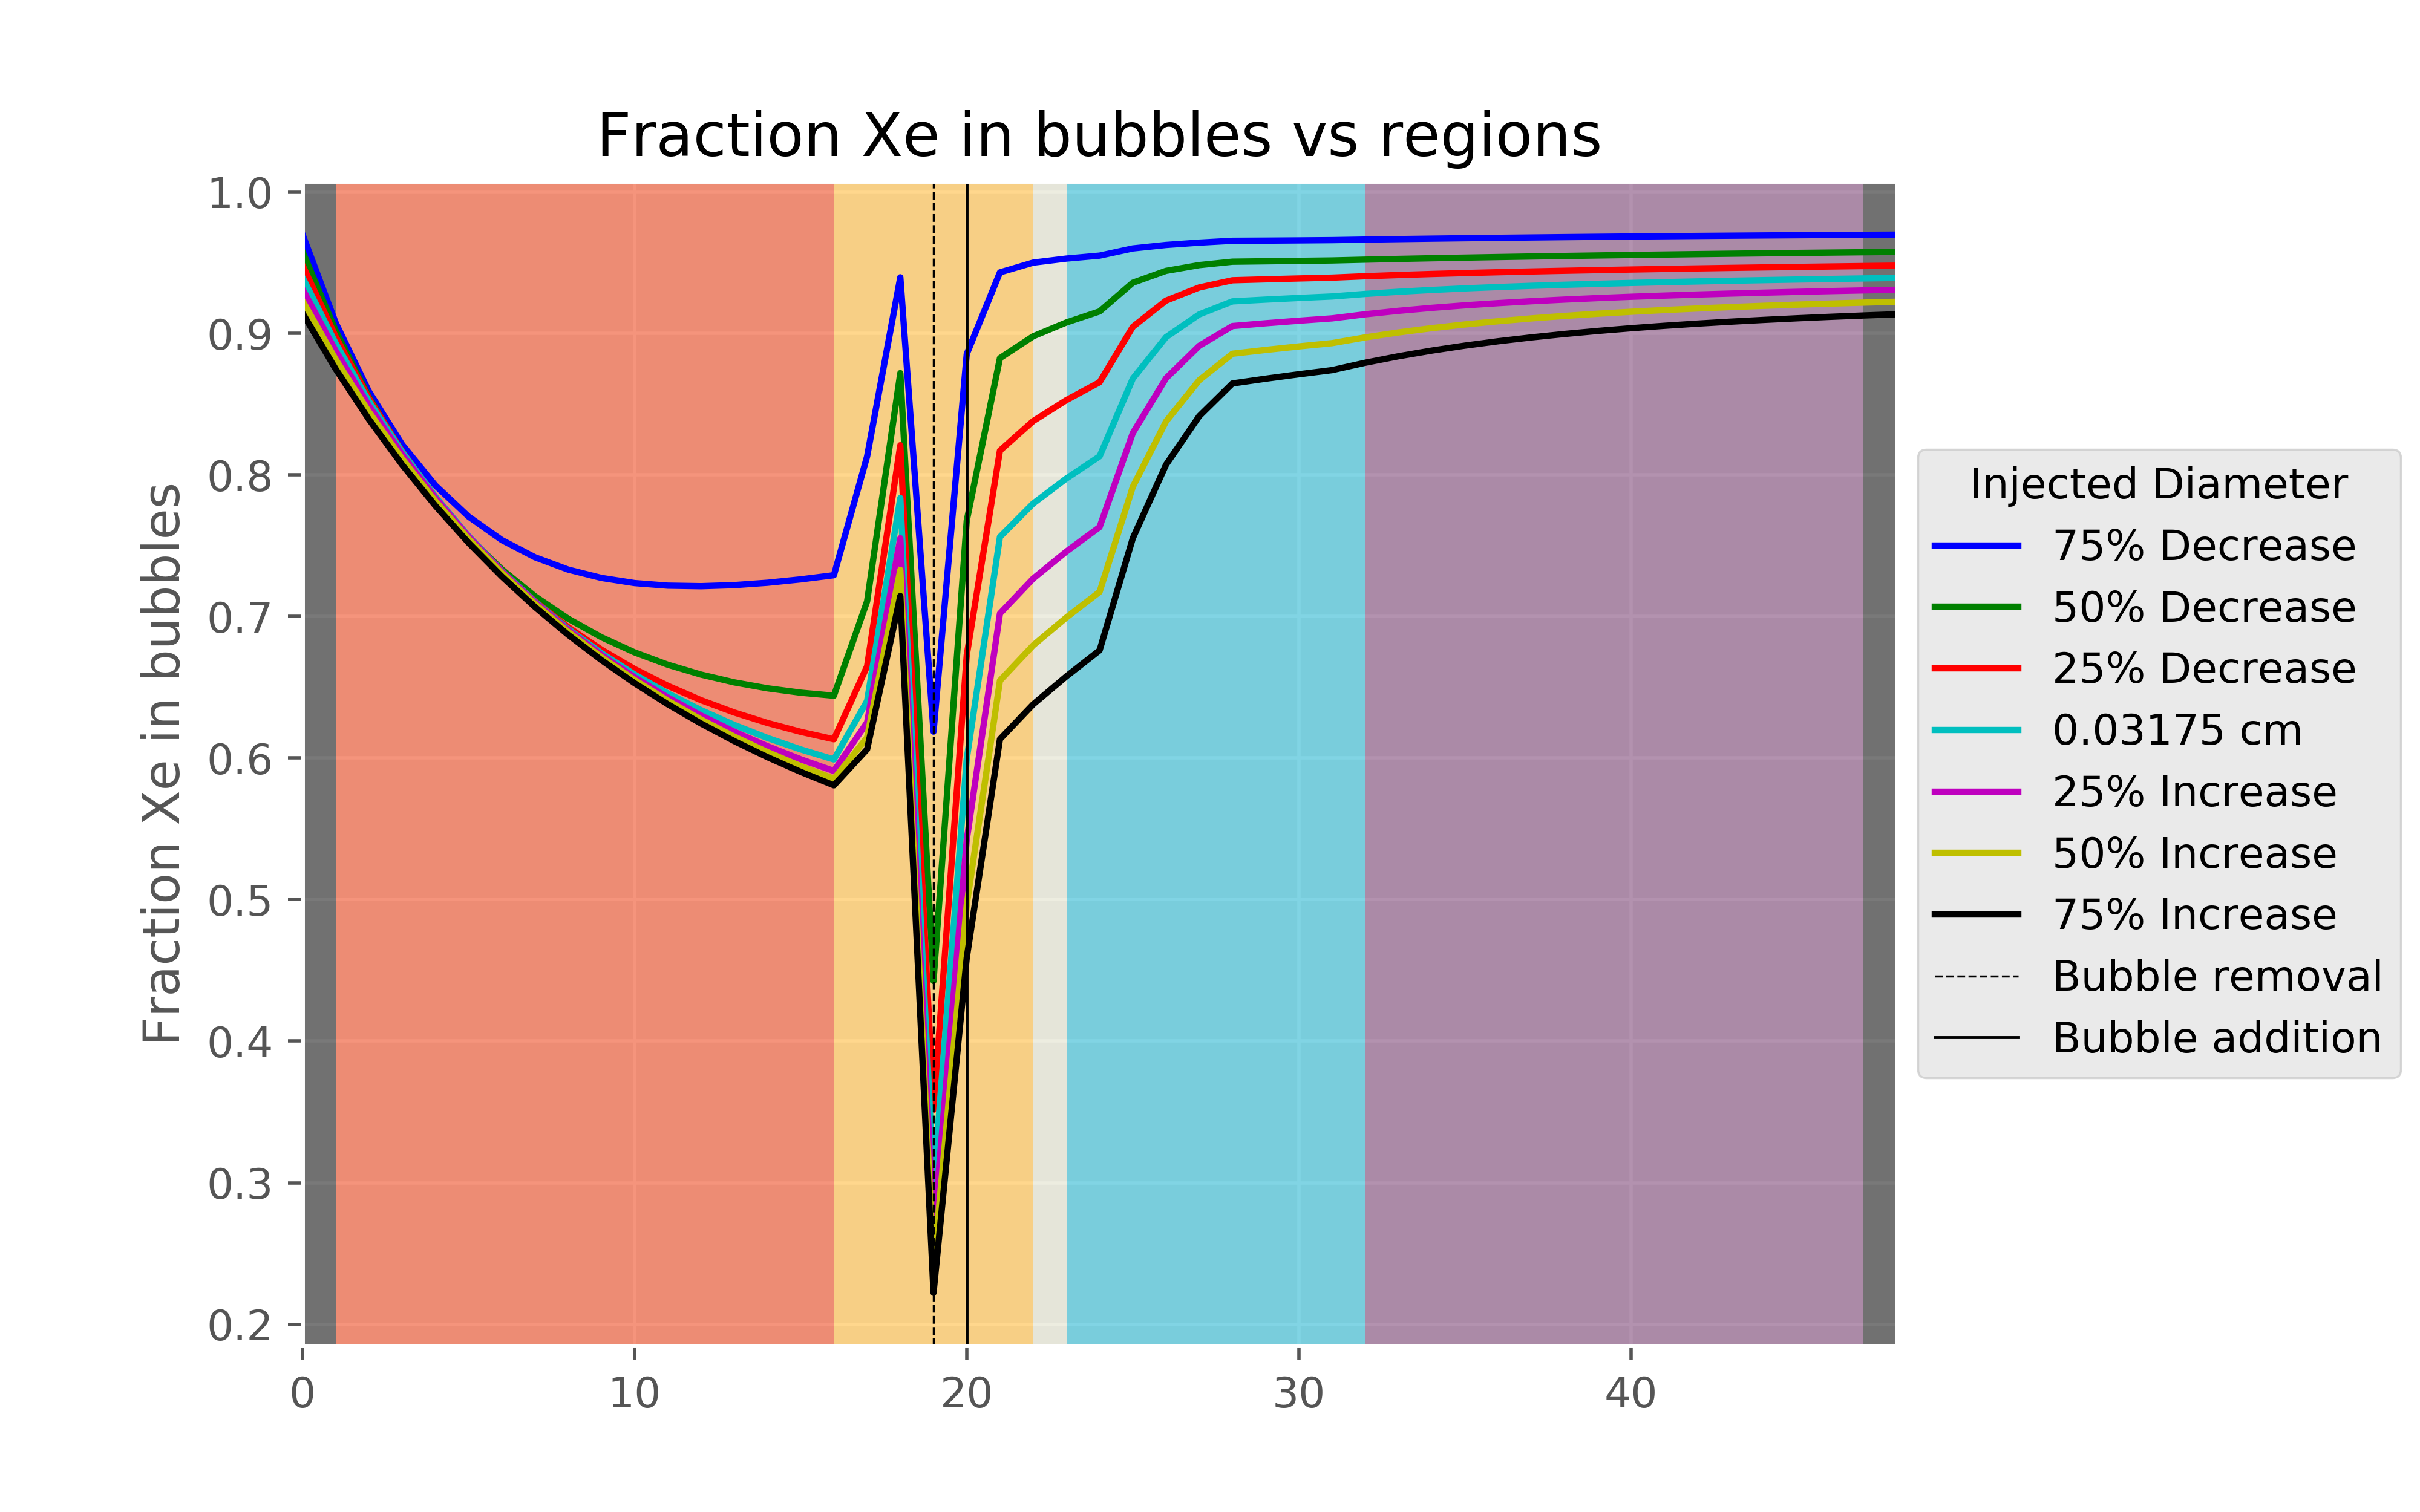
\includegraphics[width=1.0\linewidth]{images/InjectedFractionXeInBubbles.png}
  \captionof{figure}{Changes in xenon in bubbles \\ with changes in injection diameter}
  \label{fig:InjectedFractionXeInBubbles}
\end{minipage}
\end{figure}

\newpage

% HeLiq and HeGas
\begin{figure}[p] 
\centering
\begin{minipage}{.5\textwidth}
  \centering
  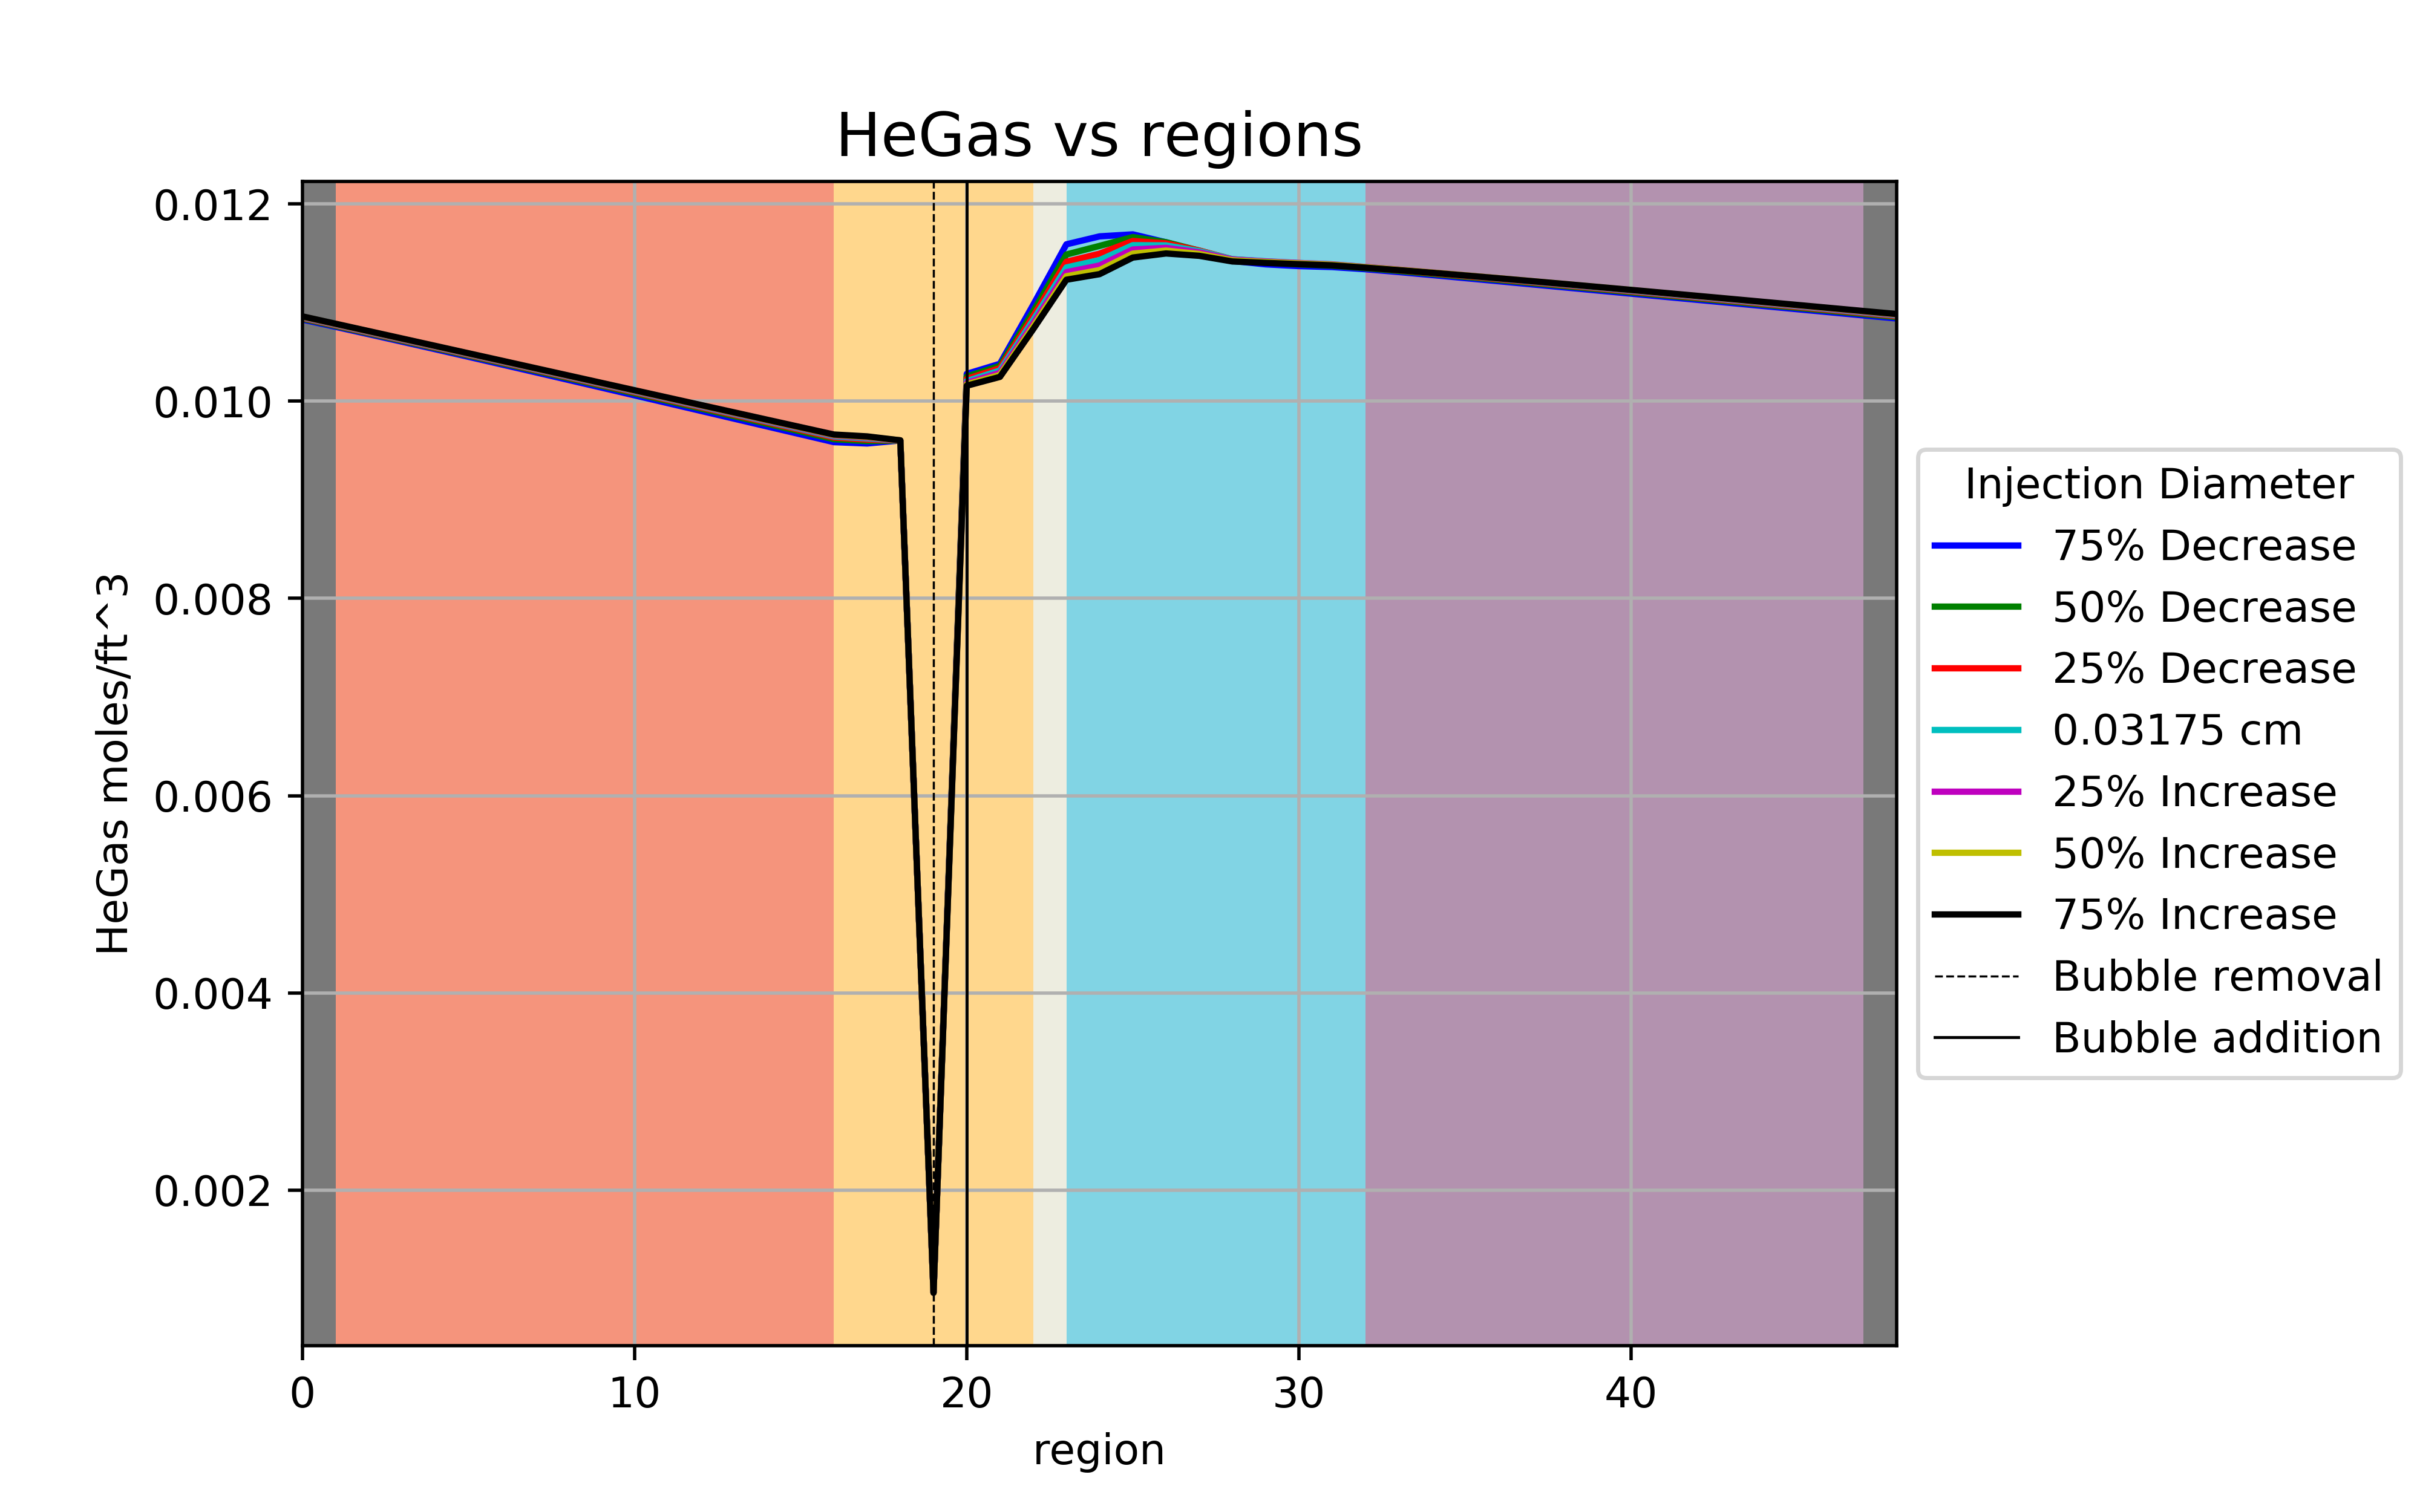
\includegraphics[width=1.0\linewidth]{images/InjectedHeGas.png}
  \captionof{figure}{Changes in helium in bubbles \\ with changes in injection diameter}
  \label{fig:InjectedHeGas}
\end{minipage}%
\begin{minipage}{.5\textwidth}
  \centering
  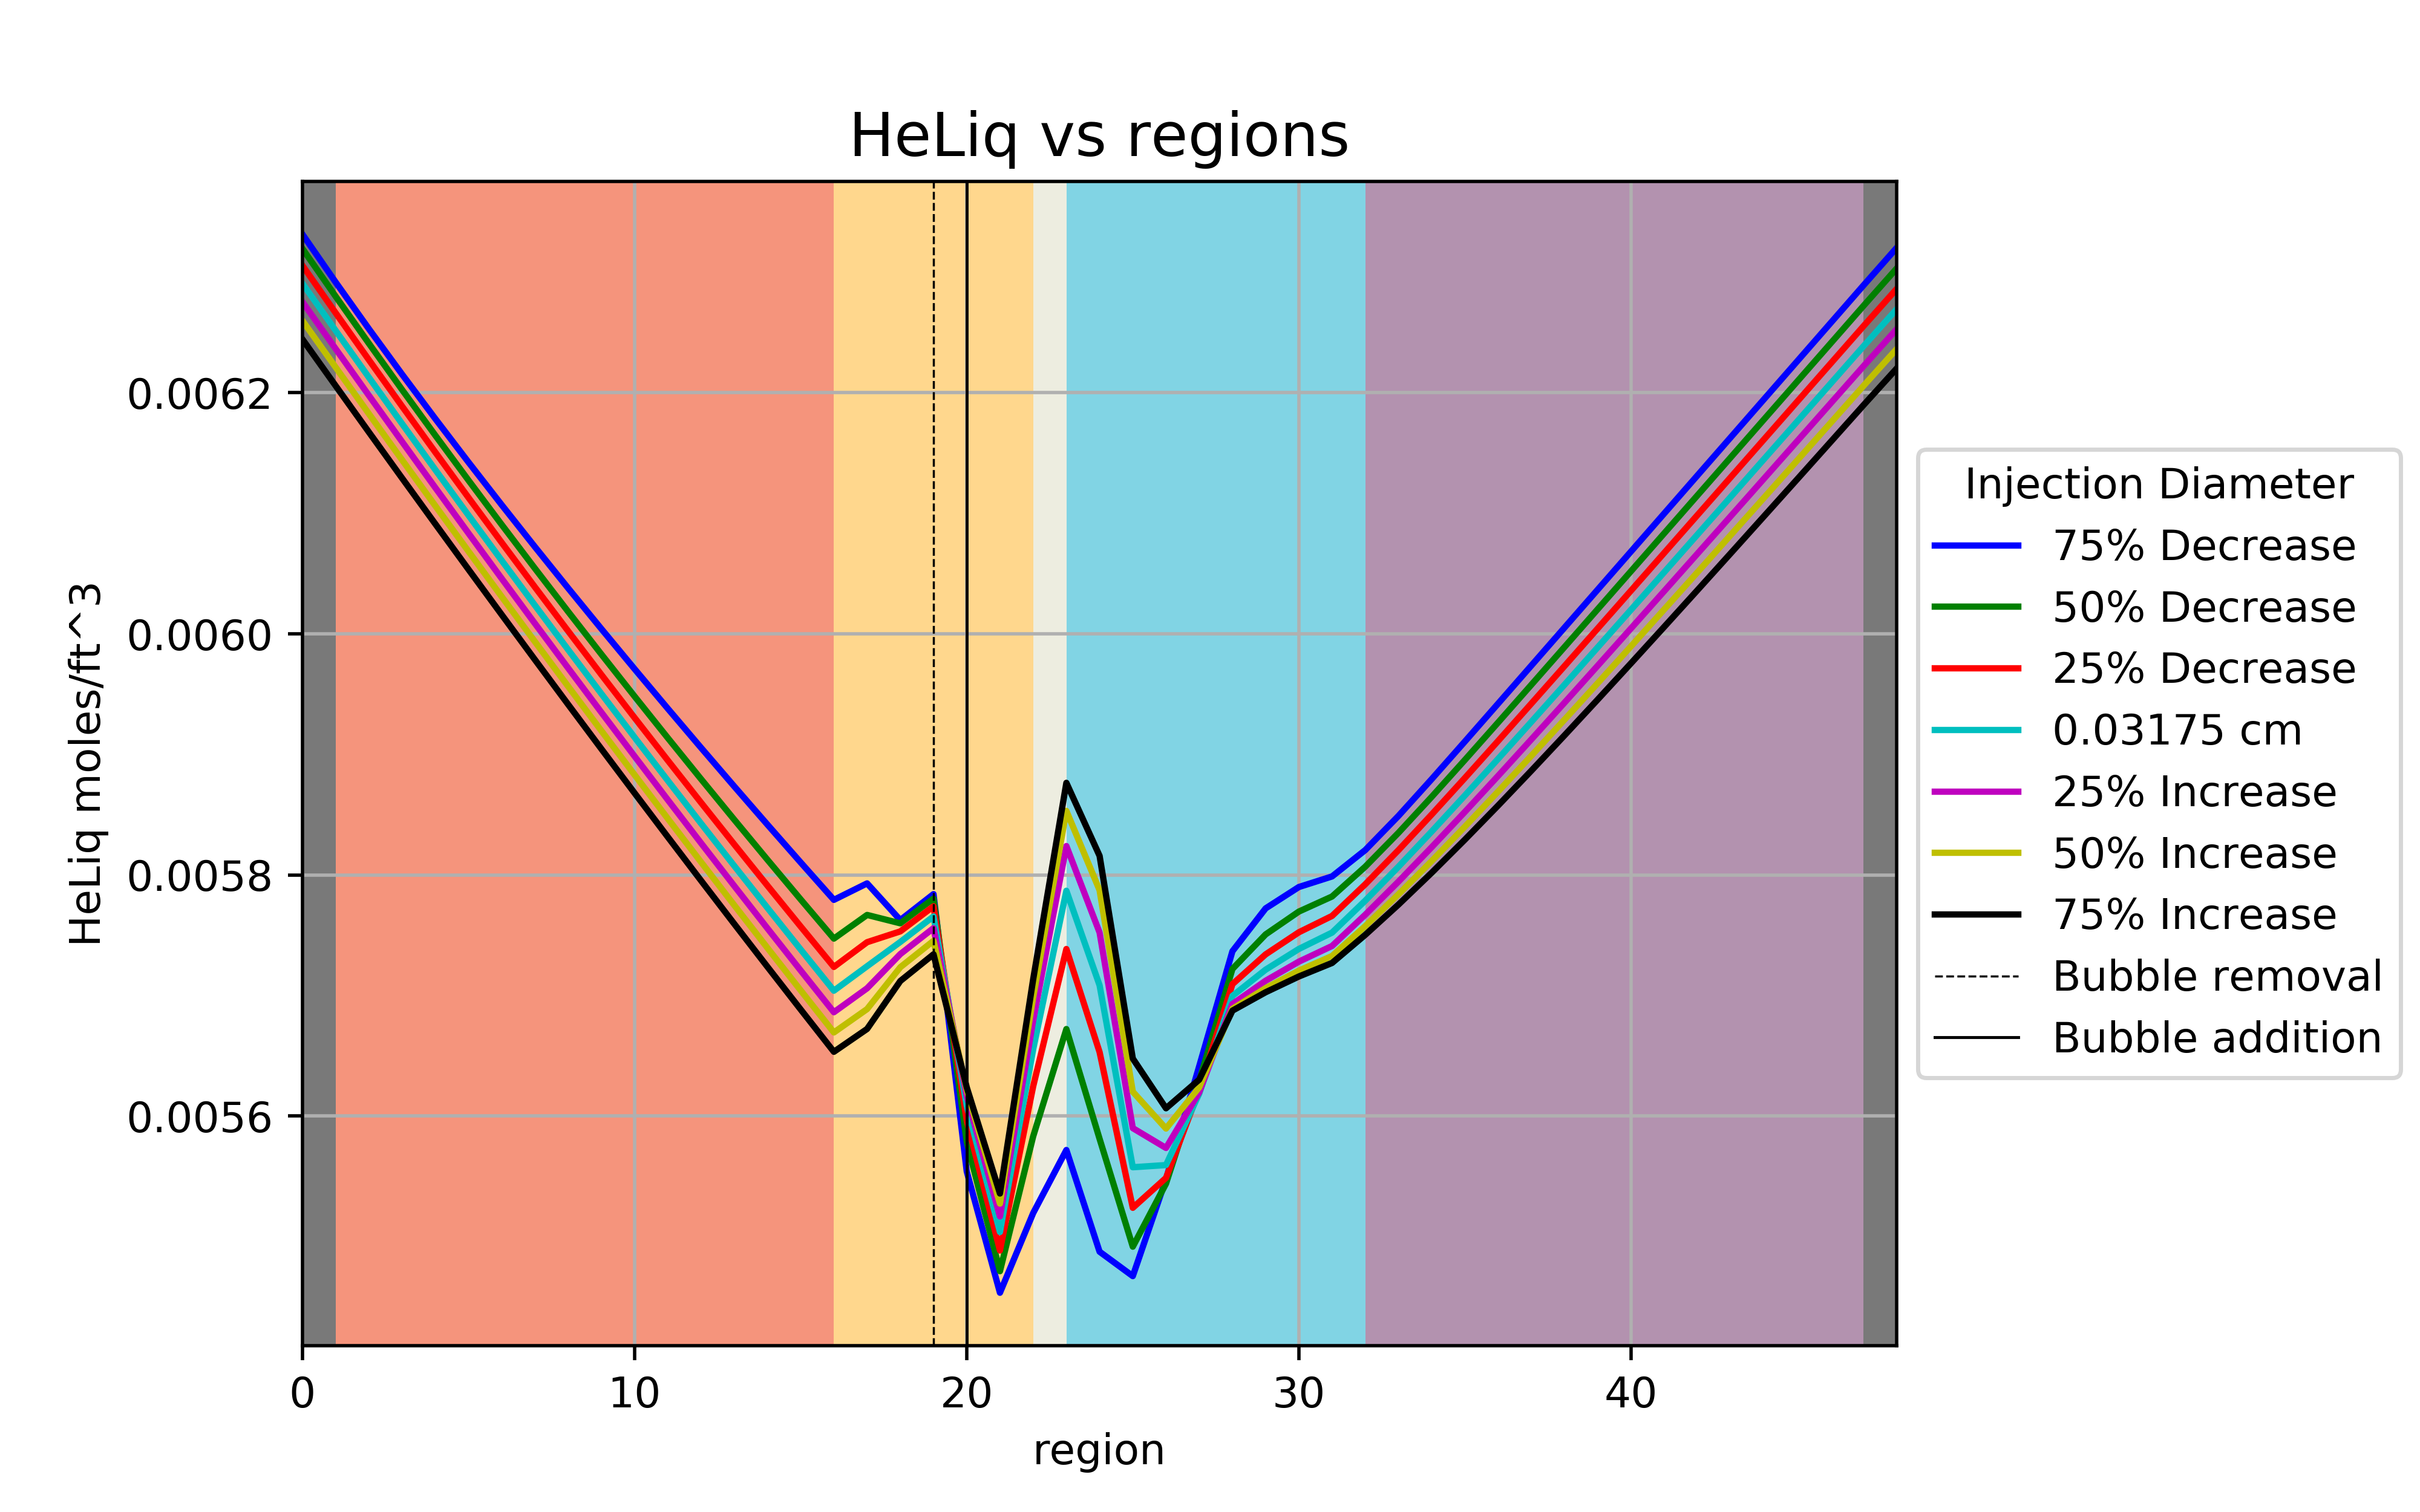
\includegraphics[width=1.0\linewidth]{images/InjectedHeLiq.png}
  \captionof{figure}{Changes in helium in the liquid \\ with changes in injection diameter}
  \label{fig:InjectedHeLiq}
\end{minipage}
\end{figure}

% XeLiq XeGas 
\begin{figure}[p] 
\centering
\begin{minipage}{.5\textwidth}
  \centering
  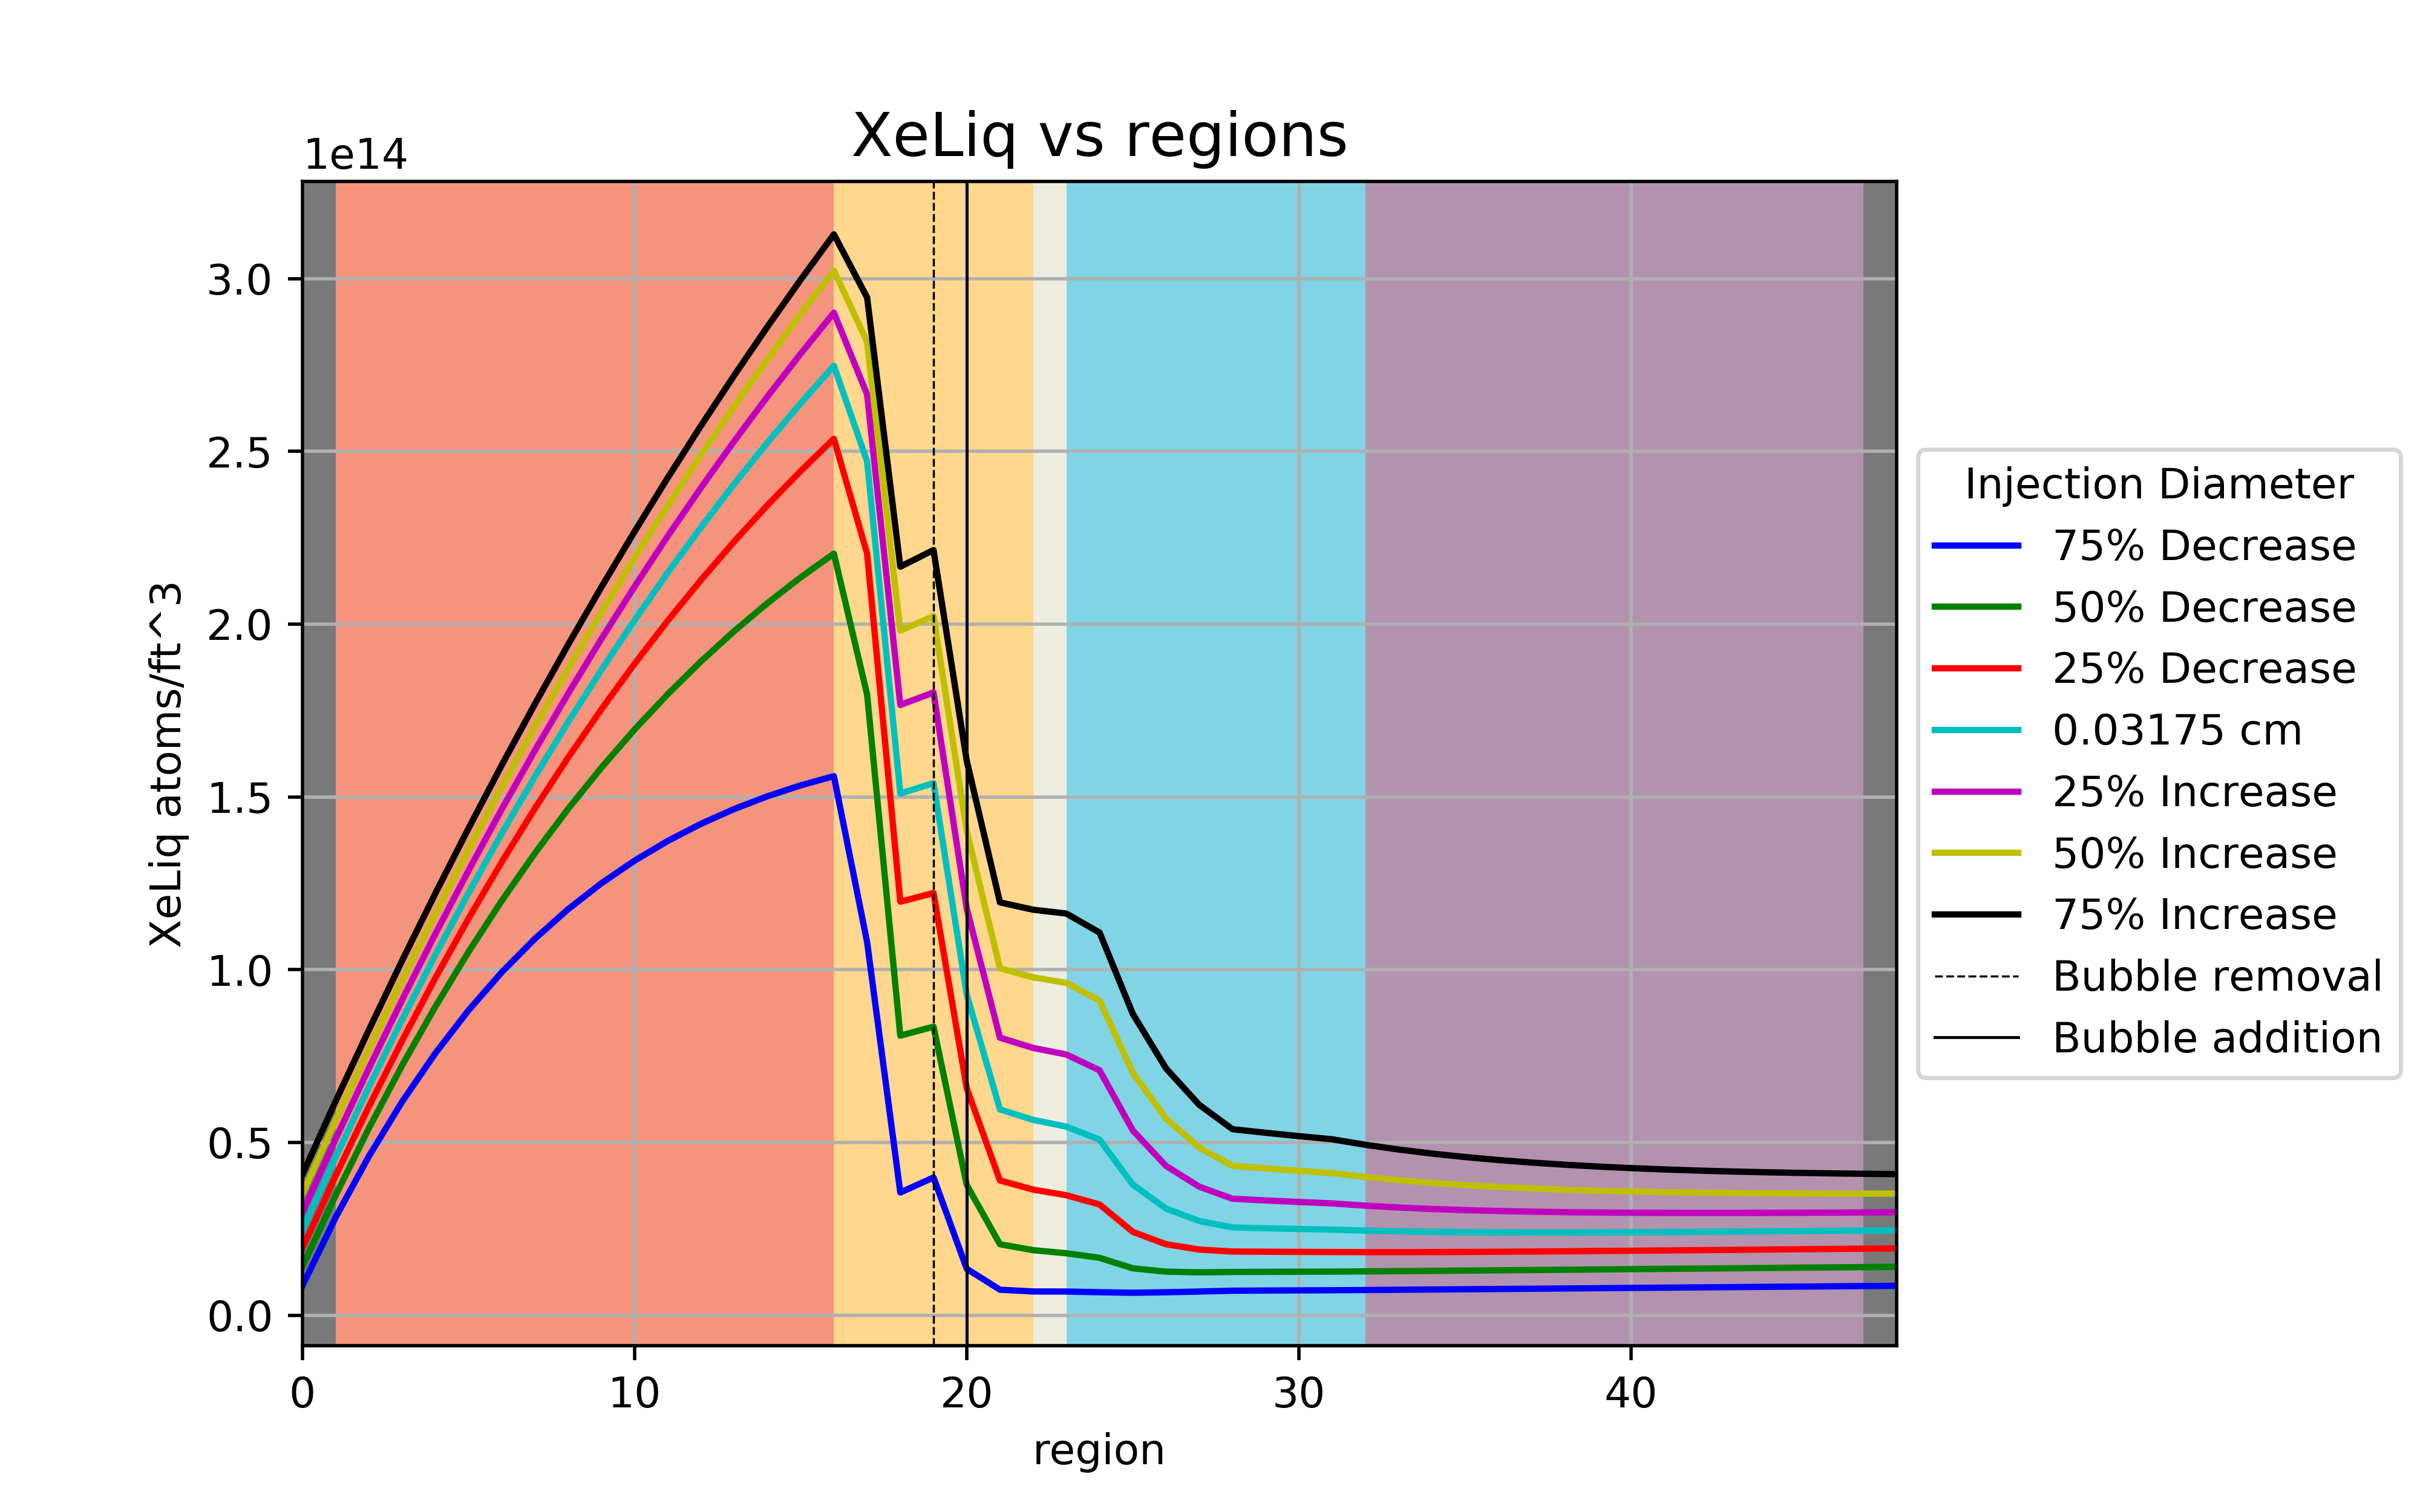
\includegraphics[width=1.0\linewidth]{images/InjectedXeLiq.png}
  \captionof{figure}{Changes in Xenon in the \\ liquid with changes in injection diameter}
  \label{fig:InjectedXeLiq}
\end{minipage}%
\begin{minipage}{.5\textwidth}
  \centering
  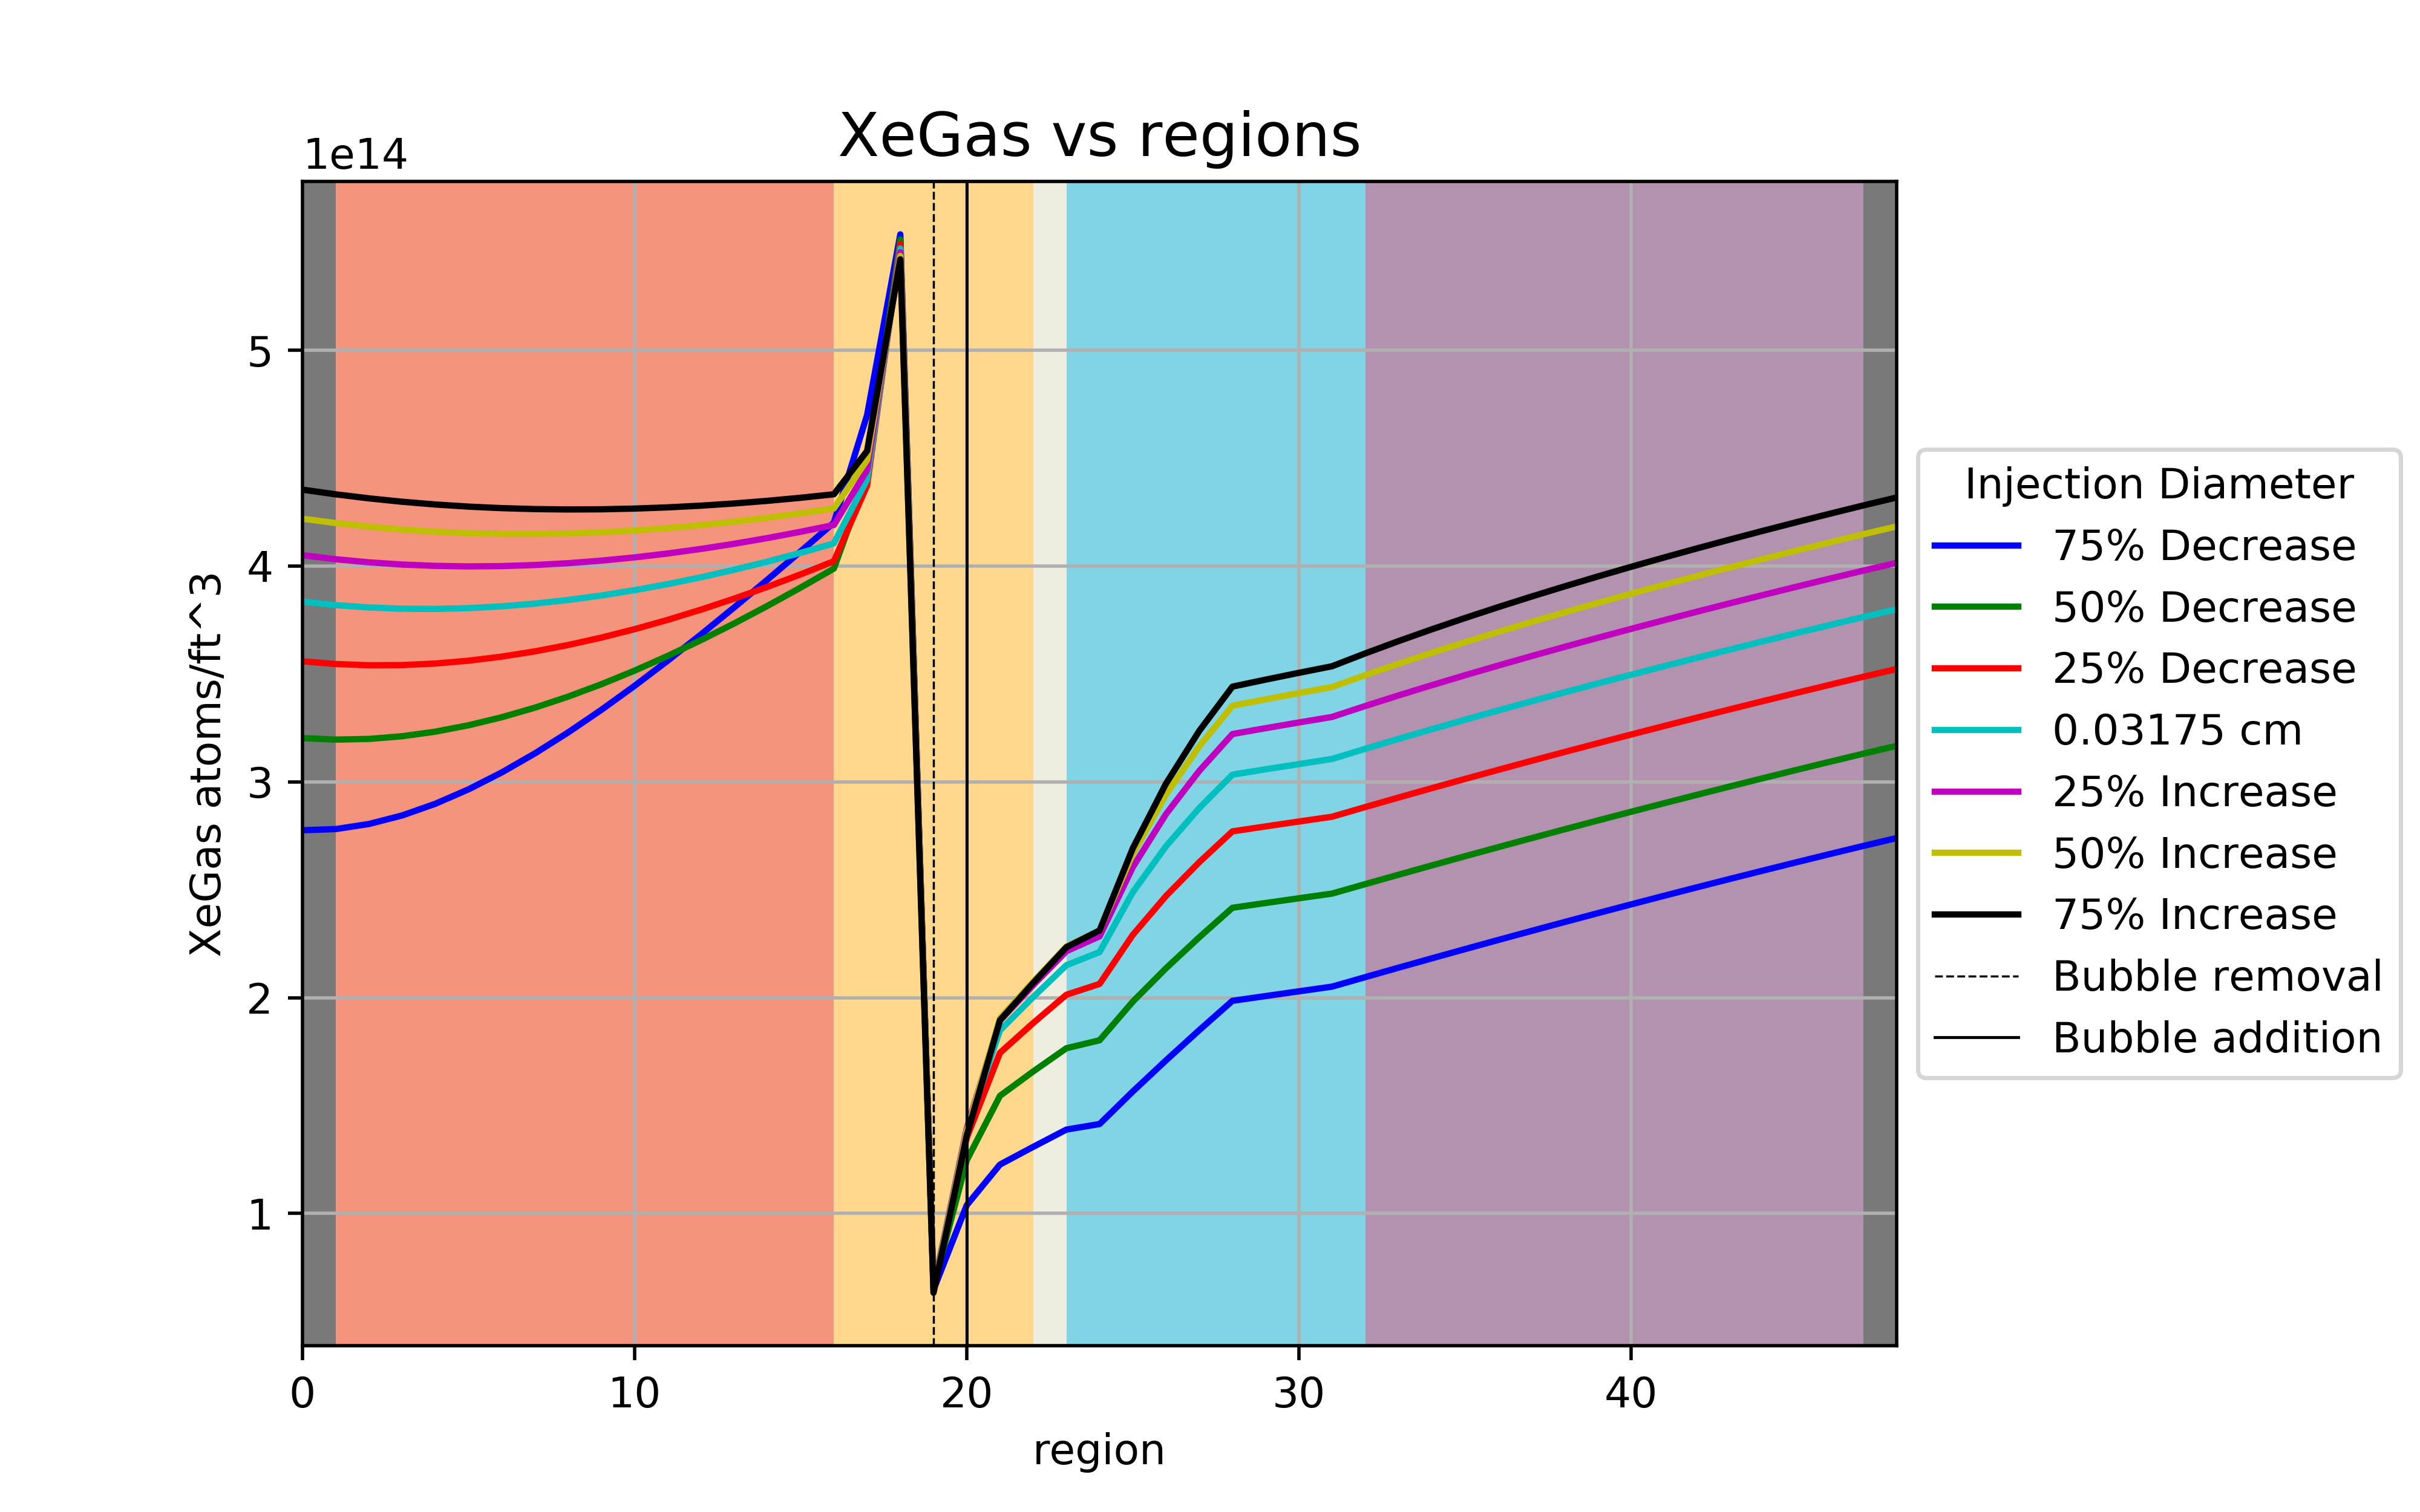
\includegraphics[width=1.0\linewidth]{images/InjectedXeGas.png}
  \captionof{figure}{Changes in Xenon in bubbles \\ with changes in injection diameter}
  \label{fig:InjectedXeGas}
\end{minipage}
\end{figure}

\FloatBarrier
\newpage

% change in mass transfer coefficient
\subsection{Change in Xenon Mass Transfer Coefficient}
The mass transfer coefficient for xenon into the gas bubbles is varied the same as the injected bubble diameter. This should only affect the xenon dissolved in liquid and trapped in the bubbles. Because more xenon is trapped in the bubbles, a slight increase in bubble diameter might be seen. This increase would only be seen if the mass of xenon in the bubbles plays a significant contribution to the over all bubble mass. As shown in Figures \ref{fig:CoeffPercentXe}, \ref{fig:CoeffXeLiq} and \ref{fig:CoeffXeGas} increasing the mass transfer coefficient will increases the amount of xenon in the bubbles and vice versa. The bubble diameter, void, and interfacial area, shown in Figures \ref{fig:CoeffDia}, \ref{fig:CoeffVoid} and \ref{fig:CoeffIntAreaCon} do not change, indicating that the mass of xenon in the bubbles isn't large enough to have an effect. The mass transfer coefficient for helium is not changed and therefor there is no change from case to case, this is shown in Figures \ref{fig:CoeffHeLiq}, \ref{fig:CoeffHeGas}.

% change in gas injection rate
\subsection{Change in Helium Gas Injection Rate}
The cover gas injection rate is varied. This will increase the overall void and interfacial area causing an increase in the amount of xenon in the bubbles. The bubble diameter is held constant and isn't expected to change however, Figure \ref{fig:RateDia} shows slight changes in bubble diameter. This change is likely due to increases mass transfer in helium from an increasing interfacial area. Shown in Figures \ref{fig:RateVoid}, \ref{fig:RateIntAreaCon} and \ref{fig:RateHeGas} void, interfacial area, helium in the bubbles all increase with increasing injection rate. What is interesting is that helium dissolved in the liquid, shown if Figure \ref{fig:RateHeLiq} increases with decreasing injection rates. Xenon trapped in the bubbles, shown if Figures \ref{fig:RatePercentXe}, \ref{fig:RateXeGas} increases with increasing injection rate as expected. As you decrease the inject rate, xenon dissolved in the liquid, Figure \ref{fig:RateXeLiq}, increases.

\vspace{12.7mm} %5mm vertical space

% void and diameter
\begin{figure}[ht] 
\centering
\begin{minipage}{.5\textwidth}
  \centering
  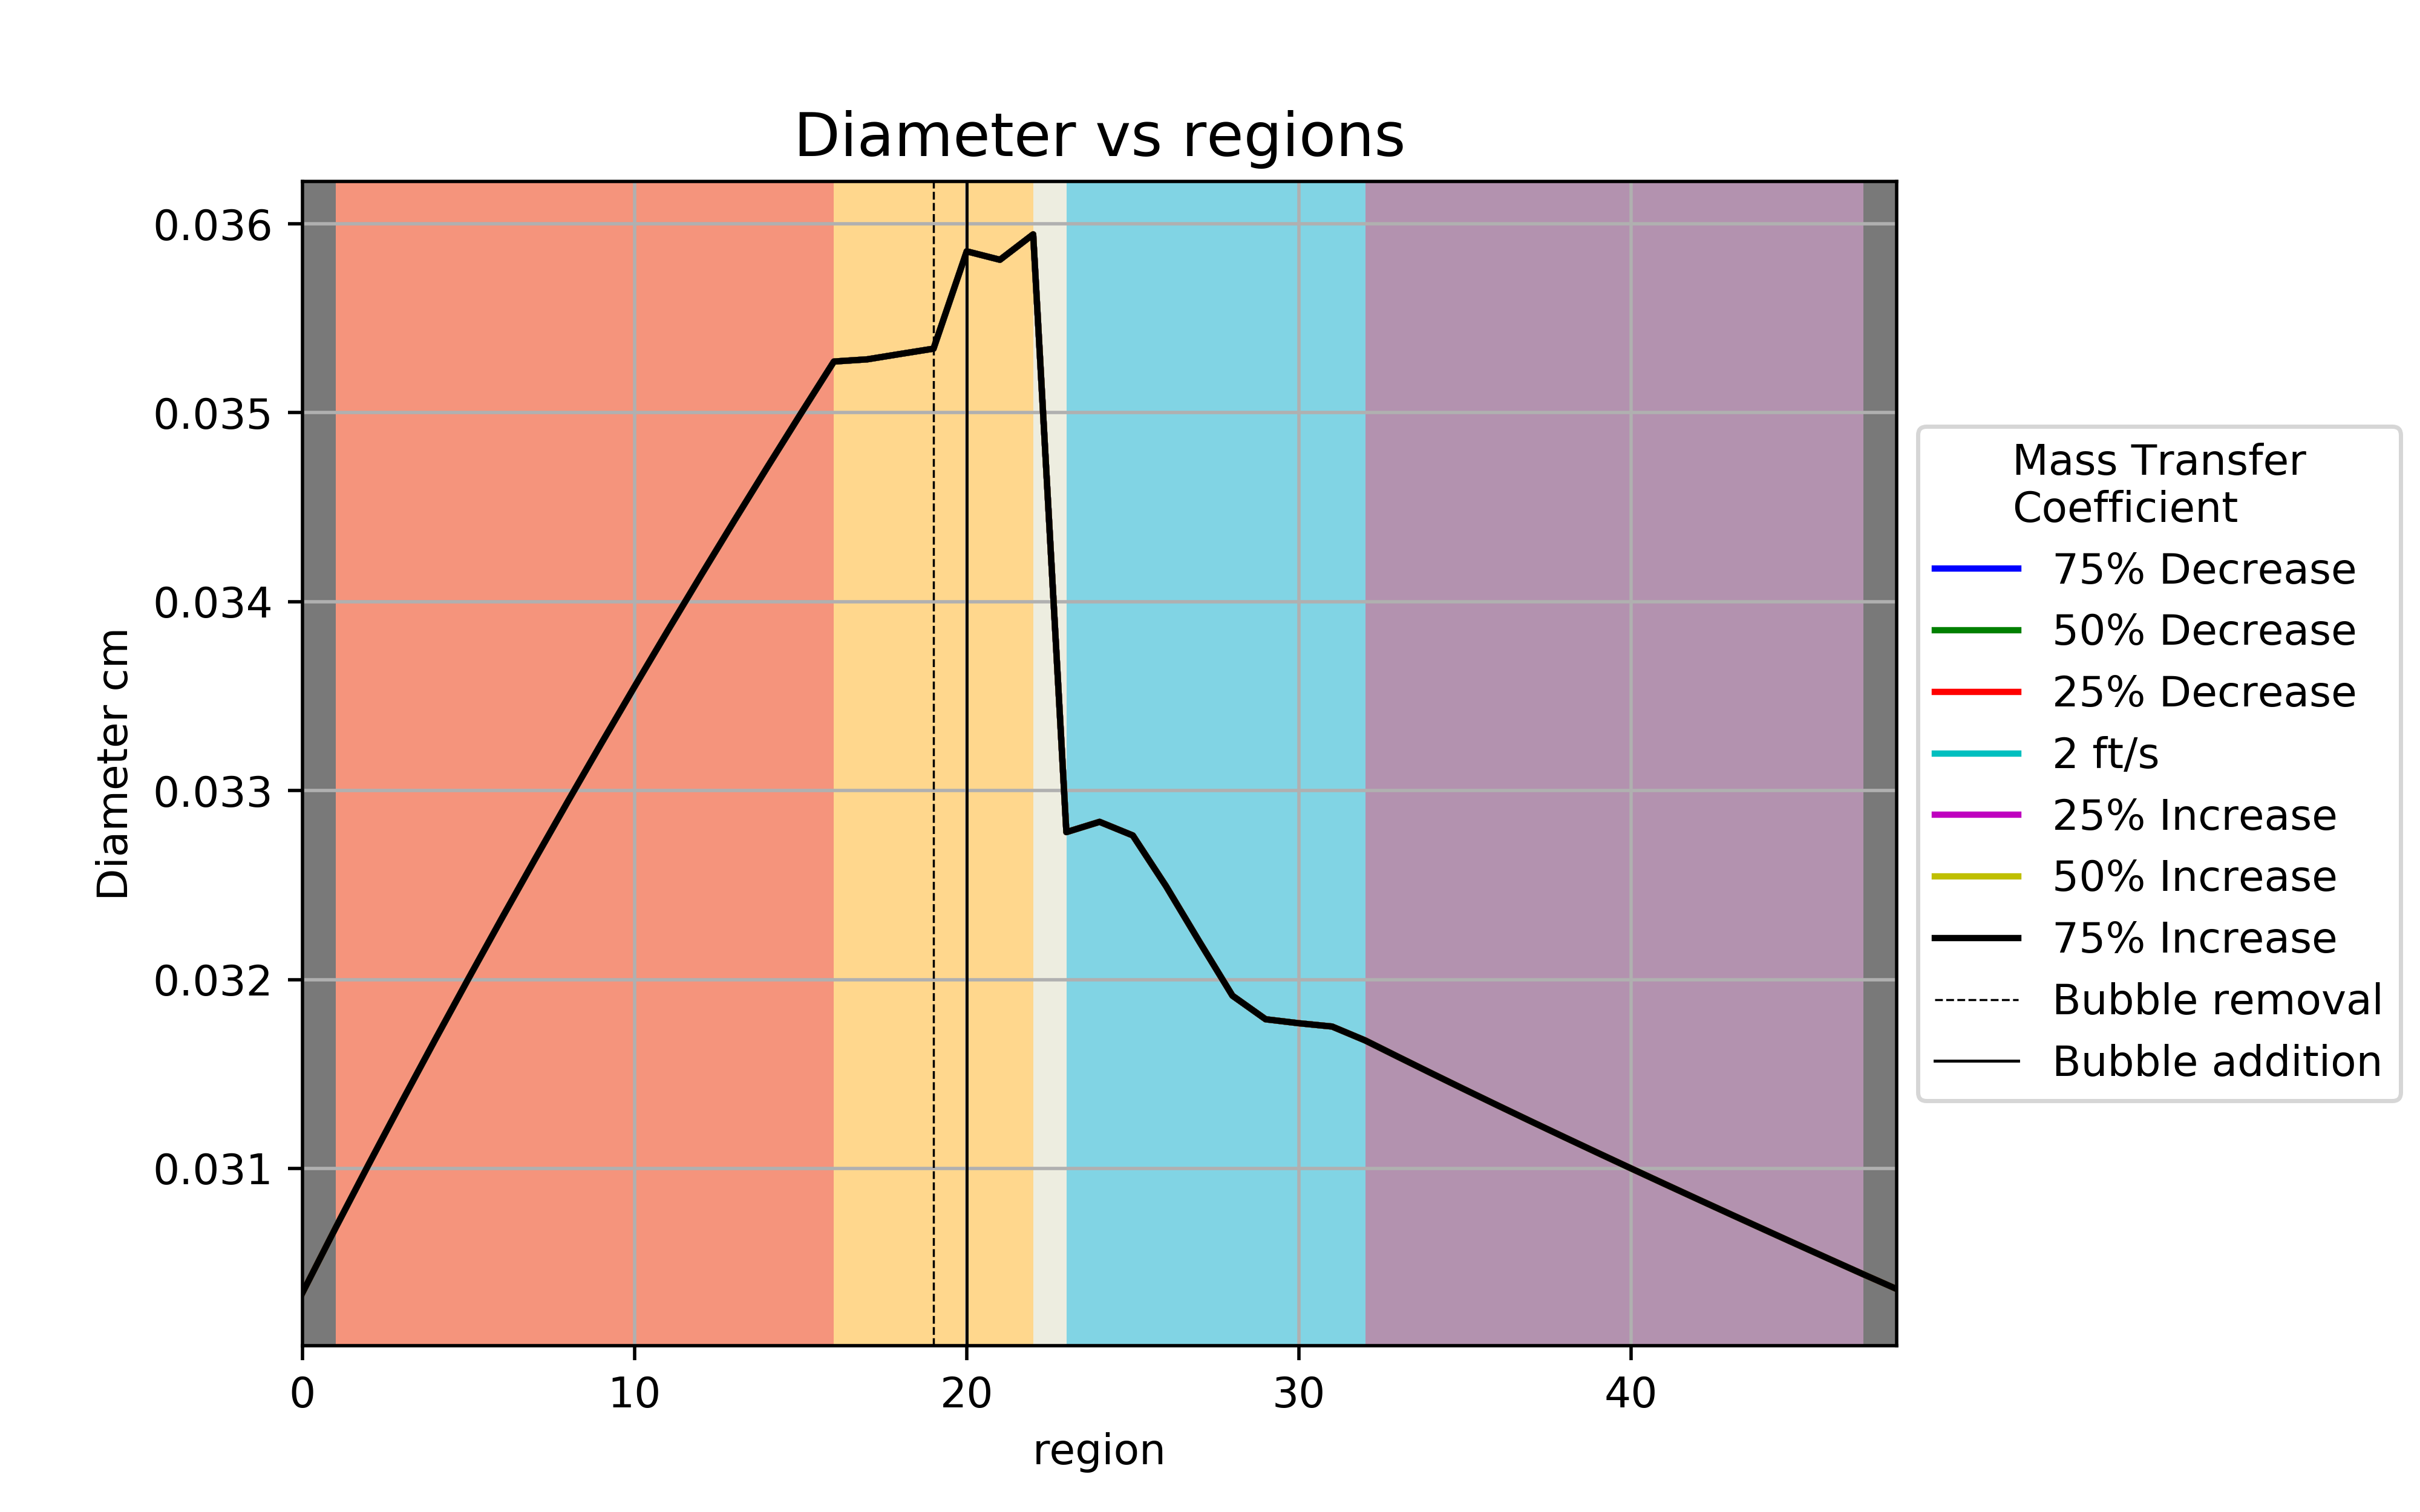
\includegraphics[width=1.0\linewidth]{images/CoeffDiameter.png}
  \captionof{figure}{Changes in bubble diameter \\ with changes in xenon mass transfer \\ coefficient}
  \label{fig:CoeffDia}
\end{minipage}%
\begin{minipage}{.5\textwidth}
  \centering
  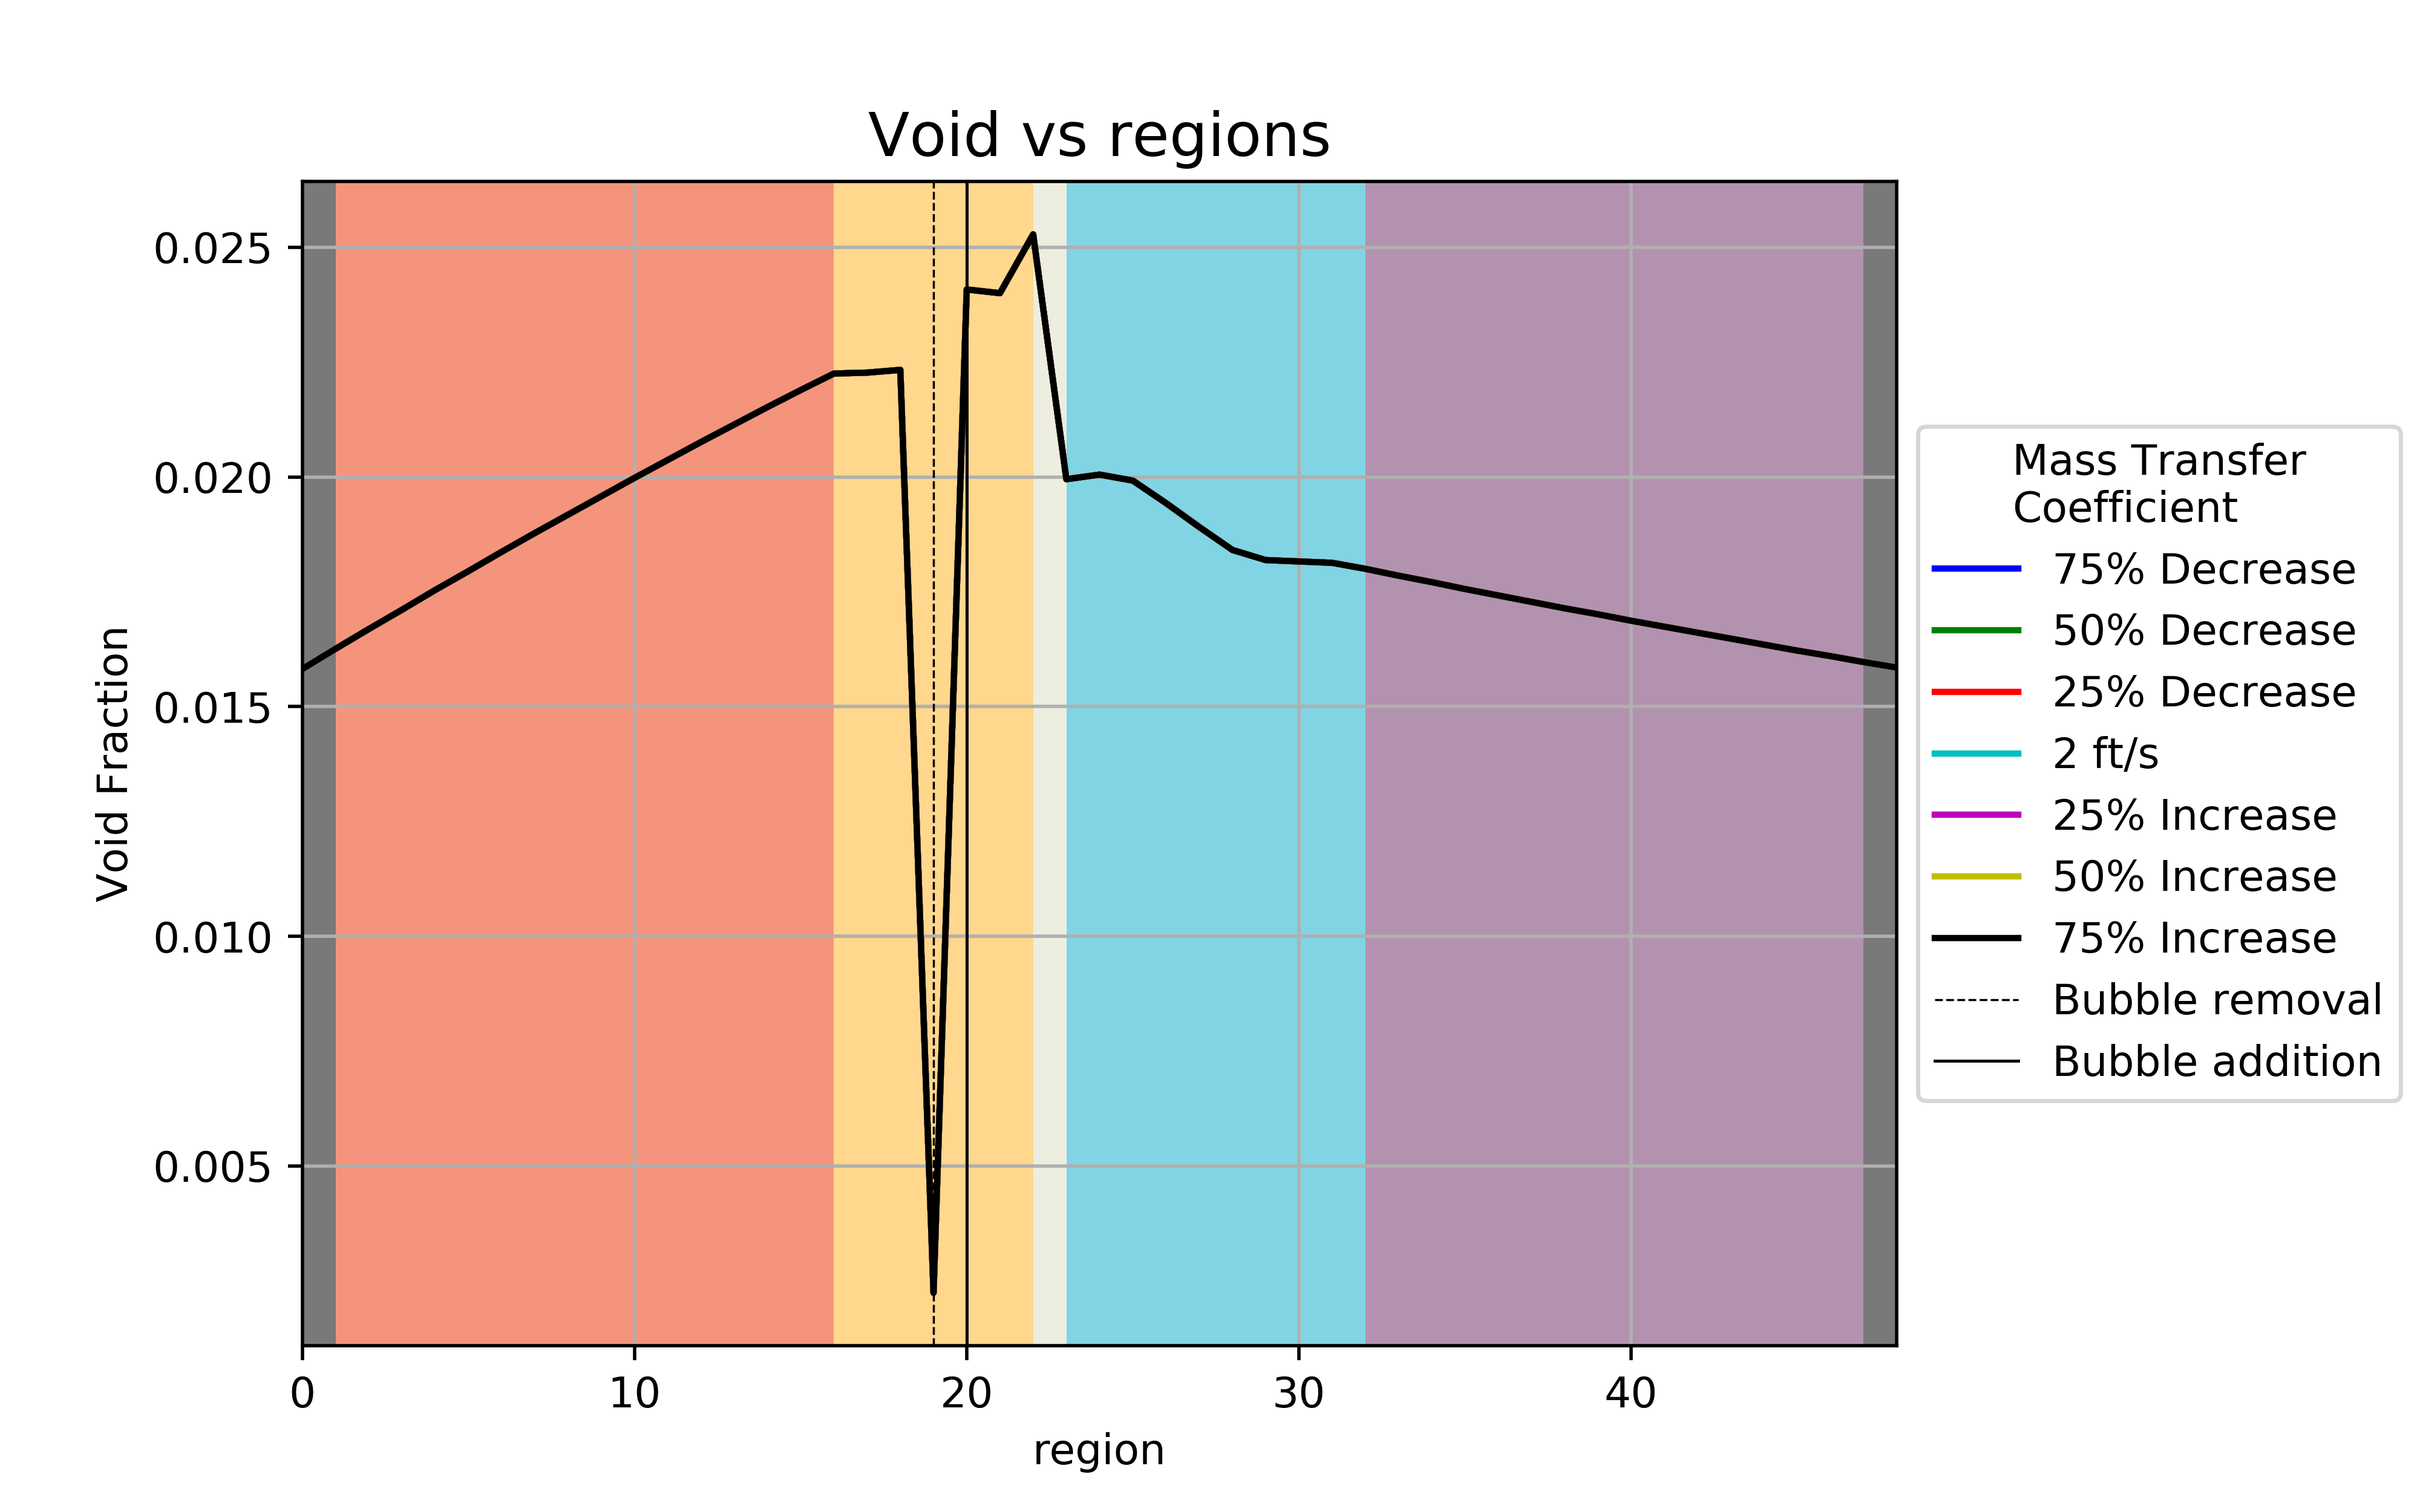
\includegraphics[width=1.0\linewidth]{images/CoeffVoid.png}
  \captionof{figure}{Changes in void fraction \\ with changes in xenon mass transfer \\ coefficient}
  \label{fig:CoeffVoid}
\end{minipage}
\end{figure}


% IntArea and Iodine
\begin{figure}[p] 
\centering
\begin{minipage}{.5\textwidth}
  \centering
  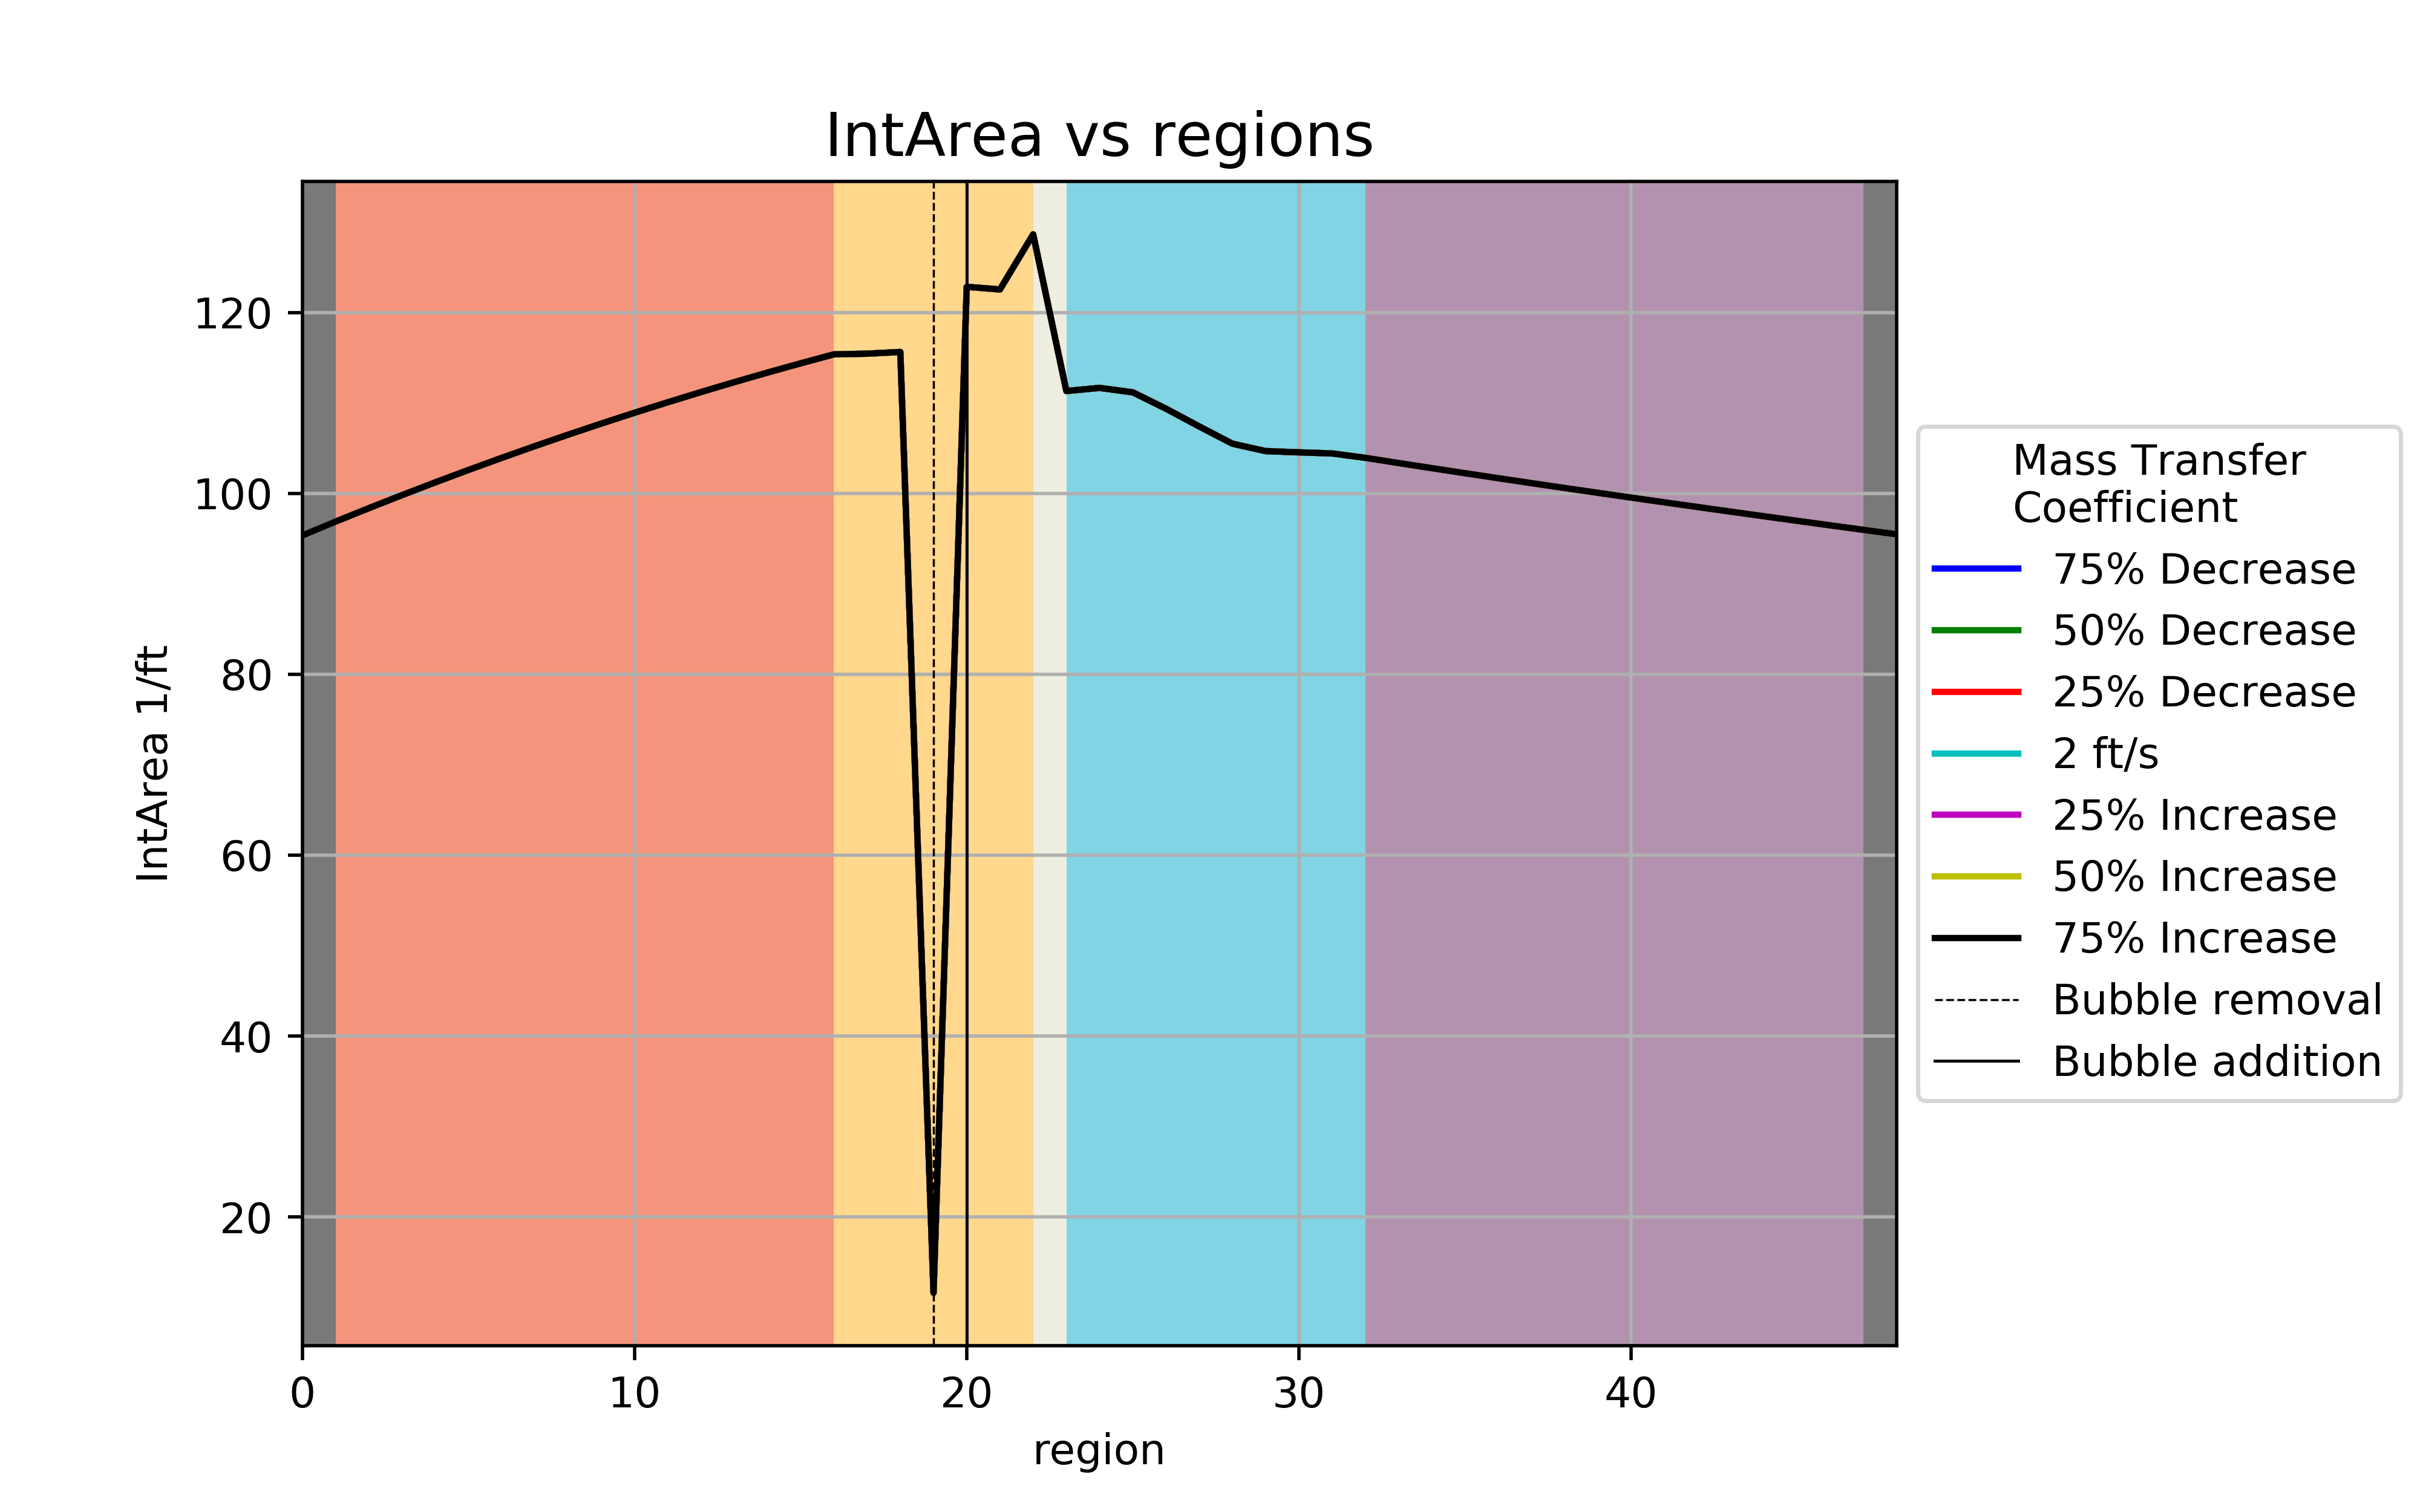
\includegraphics[width=1.0\linewidth]{images/CoeffIntArea.png}
  \captionof{figure}{Changes in interfacial area \\ with changes in xenon mass transfer \\ coefficient}
  \label{fig:CoeffIntAreaCon}
\end{minipage}%
\begin{minipage}{.5\textwidth}
  \centering
  \includegraphics[width=1.0\linewidth]{images/CoeffFractionXeInBubbles.png}
  \captionof{figure}{Changes in xenon in bubbles \\ with changes in xenon mass transfer \\ coefficient}
  \label{fig:CoeffPercentXe}
\end{minipage}
\end{figure}

\FloatBarrier
\newpage
\FloatBarrier

% HeLiq and HeGas
\begin{figure}[p] 
\centering
\begin{minipage}{.5\textwidth}
  \centering
  \includegraphics[width=1.0\linewidth]{images/CoeffHeGas.png}
  \captionof{figure}{Changes in helium in bubbles \\ with changes in xenon mass transfer \\ coefficient}
  \label{fig:CoeffHeGas}
\end{minipage}%
\begin{minipage}{.5\textwidth}
  \centering
  \includegraphics[width=1.0\linewidth]{images/CoeffHeLiq.png}
  \captionof{figure}{Changes in helium in the liquid \\ with changes in xenon mass transfer \\ coefficient}
  \label{fig:CoeffHeLiq}
\end{minipage}
\end{figure}

% XeLiq XeGas 
\begin{figure}[p] 
\centering
\begin{minipage}{.5\textwidth}
  \centering
  \includegraphics[width=1.0\linewidth]{images/CoeffXeLiq.png}
  \captionof{figure}{Changes in Xenon in the \\ liquid with changes in xenon mass transfer \\ coefficient}
  \label{fig:CoeffXeLiq}
\end{minipage}%
\begin{minipage}{.5\textwidth}
  \centering
  \includegraphics[width=1.0\linewidth]{images/CoeffXeGas.png}
  \captionof{figure}{Changes in Xenon in bubbles \\ with changes in xenon mass transfer \\ coefficient}
  \label{fig:CoeffXeGas}
\end{minipage}
\end{figure}

\FloatBarrier
\newpage
\FloatBarrier


% cover gas injection rate
% void and diameter
\begin{figure}[p] 
\centering
\begin{minipage}{.5\textwidth}
  \centering
  \includegraphics[width=1.0\linewidth]{images/RateDiameter.png}
  \captionof{figure}{Changes in bubble diameter \\ with changes in cover gas injection rate}
  \label{fig:RateDia}
\end{minipage}%
\begin{minipage}{.5\textwidth}
  \centering
  \includegraphics[width=1.0\linewidth]{images/RateVoid.png}
  \captionof{figure}{Changes in void fraction \\ with changes in cover gas injection rate}
  \label{fig:RateVoid}
\end{minipage}
\end{figure}

% IntArea and Iodine
\begin{figure}[p] 
\centering
\begin{minipage}{.5\textwidth}
  \centering
  \includegraphics[width=1.0\linewidth]{images/RateIntArea.png}
  \captionof{figure}{Changes in interfacial area \\ with changes in cover gas injection rate}
  \label{fig:RateIntAreaCon}
\end{minipage}%
\begin{minipage}{.5\textwidth}
  \centering
  \includegraphics[width=1.0\linewidth]{images/RateFractionXeInBubbles.png}
  \captionof{figure}{Changes in xenon in bubbles \\ with changes in cover gas injection rate}
  \label{fig:RatePercentXe}
\end{minipage}
\end{figure}

\FloatBarrier
\newpage
\FloatBarrier

% HeLiq and HeGas
\begin{figure}[p] 
\centering
\begin{minipage}{.5\textwidth}
  \centering
  \includegraphics[width=1.0\linewidth]{images/RateHeGas.png}
  \captionof{figure}{Changes in helium in bubbles \\ with changes in cover gas injection rate}
  \label{fig:RateHeGas}
\end{minipage}%
\begin{minipage}{.5\textwidth}
  \centering
  \includegraphics[width=1.0\linewidth]{images/RateHeLiq.png}
  \captionof{figure}{Changes in helium in the liquid \\ with changes in cover gas injection rate}
  \label{fig:RateHeLiq}
\end{minipage}
\end{figure}

% XeLiq XeGas 
\begin{figure}[p] 
\centering
\begin{minipage}{.5\textwidth}
  \centering
  \includegraphics[width=1.0\linewidth]{images/RateXeLiq.png}
  \captionof{figure}{Changes in Xenon in the \\ liquid with changes in cover gas injection \\ rate}
  \label{fig:RateXeLiq}
\end{minipage}%
\begin{minipage}{.5\textwidth}
  \centering
  \includegraphics[width=1.0\linewidth]{images/RateXeGas.png}
  \captionof{figure}{Changes in Xenon in bubbles \\ with changes in cover gas injection \\ rate}
  \label{fig:RateXeGas}
\end{minipage}
\end{figure}

\FloatBarrier
\newpage
\FloatBarrier

\subsection{Bubble Removal Efficiency}
The bubble removal efficiency is varied from 1\% to 99\% in 5 steps. Results are shown in Figures \ref{fig:EffDia} to \ref{fig:EffXeGas}. Bubble diameter increases with increasing removal efficiency, shown in Figure \ref{fig:EffDia}, this can be attributed to increasing the residence time for mass transfer for a single bubble. The void fraction, shown in Figure \ref{fig:EffVoid}, increases with decreasing removal efficiency. A likely cause for this increase is due to not removing as many bubbles, thus increasing the steady state void. As removal efficiency is increased less bubbles are present resulting in a decrease in interfacial area and helium in the bubbles shown in Figures \ref{fig:EffIntAreaCon}, \ref{fig:EffHeLiq} and \ref{fig:EffHeGas}. With higher efficiency more of helium and xenon will be in the liquid, which is shown in Figures \ref{fig:EffPercentXe}, \ref{fig:EffXeLiq} and \ref{fig:EffXeGas}. What is interesting is that as you increase the efficiency you decrease the amount of xenon in the bubbles and the percent of xenon in the bubbles approaches unity. This behavior is due to the bubbles being able to spend more time in the loop resulting in more xenon transporting into said bubbles. 

\subsection{Change in Cover Gas}
Argon was another cover gas utilized in the MSRE. The primary difference between helium and argon is from the order of magnitude decrease in solubility of argon in the molten salt. This means that less argon will transport out of the bubbles and into the liquid. As a result the bubble will better hold its identity under pressure changes. Results are shown in Figures \ref{fig:CoverGasDia} to \ref{fig:CoverGasXeGas}. As shown in the results, changes between the two gases are minimal. Helium dissolves more in the molten salt and is shown in Figure \ref{fig:CoverGasHeLiq}. Bubble diameter seems to slightly change after the heat exchanger with the argon bubbles being less affected by pressure changes, this is shown in the void, diameter and interfacial area, Figures \ref{fig:CoverGasVoid}, \ref{fig:CoverGasDia} and \ref{fig:CoverGasIntAreaCon}. This is seen by the increase in bubble diameter. Changes in the fraction of xenon in the bubbles, xenon in the bubbles and xenon in the liquid shown in Figures \ref{fig:CoverGasPercentXe}, \ref{fig:CoverGasXeGas} and \ref{fig:CoverGasXeLiq}, are not noticeable. 

\FloatBarrier
\newpage
\FloatBarrier

% void and diameter
\begin{figure}[p] 
\centering
\begin{minipage}{.5\textwidth}
  \centering
  \includegraphics[width=1.0\linewidth]{images/EffDiameter.png}
  \captionof{figure}{Changes in bubble diameter \\ with changes in removal efficiency}
  \label{fig:EffDia}
\end{minipage}%
\begin{minipage}{.5\textwidth}
  \centering
  \includegraphics[width=1.0\linewidth]{images/EffVoid.png}
  \captionof{figure}{Changes in void fraction \\ with changes in removal efficiency}
  \label{fig:EffVoid}
\end{minipage}
\end{figure}

% IntArea and Iodine
\begin{figure}[p] 
\centering
\begin{minipage}{.5\textwidth}
  \centering
  \includegraphics[width=1.0\linewidth]{images/EffIntArea.png}
  \captionof{figure}{Changes in interfacial area \\ with changes in removal efficiency}
  \label{fig:EffIntAreaCon}
\end{minipage}%
\begin{minipage}{.5\textwidth}
  \centering
  \includegraphics[width=1.0\linewidth]{images/EffFractionXeInBubbles.png}
  \captionof{figure}{Changes in xenon in bubbles \\ with changes in removal efficiency}
  \label{fig:EffPercentXe}
\end{minipage}
\end{figure}

\FloatBarrier
\newpage
\FloatBarrier

% HeLiq and HeGas
\begin{figure}[p] 
\centering
\begin{minipage}{.5\textwidth}
  \centering
  \includegraphics[width=1.0\linewidth]{images/EffHeGas.png}
  \captionof{figure}{Changes in helium in bubbles \\ with changes in removal efficiency}
  \label{fig:EffHeGas}
\end{minipage}%
\begin{minipage}{.5\textwidth}
  \centering
  \includegraphics[width=1.0\linewidth]{images/EffHeLiq.png}
  \captionof{figure}{Changes in helium in the liquid \\ with changes in removal efficiency}
  \label{fig:EffHeLiq}
\end{minipage}
\end{figure}

% XeLiq XeGas 
\begin{figure}[p] 
\centering
\begin{minipage}{.5\textwidth}
  \centering
  \includegraphics[width=1.0\linewidth]{images/EffXeLiq.png}
  \captionof{figure}{Changes in Xenon in the \\ liquid with changes in removal efficiency}
  \label{fig:EffXeLiq}
\end{minipage}%
\begin{minipage}{.5\textwidth}
  \centering
  \includegraphics[width=1.0\linewidth]{images/EffXeGas.png}
  \captionof{figure}{Changes in Xenon in bubbles \\ with changes in removal efficiency}
  \label{fig:EffXeGas}
\end{minipage}
\end{figure}

\FloatBarrier
\newpage
\FloatBarrier


% cover gas 
% void and diameter
\begin{figure}[p] 
\centering
\begin{minipage}{.5\textwidth}
  \centering
  \includegraphics[width=1.0\linewidth]{images/CoverGasDiameter.png}
  \captionof{figure}{Changes in bubble diameter \\ with changes in cover gas}
  \label{fig:CoverGasDia}
\end{minipage}%
\begin{minipage}{.5\textwidth}
  \centering
  \includegraphics[width=1.0\linewidth]{images/CoverGasVoid.png}
  \captionof{figure}{Changes in void fraction \\ with changes in cover gas}
  \label{fig:CoverGasVoid}
\end{minipage}
\end{figure}

% IntArea and Iodine
\begin{figure}[p] 
\centering
\begin{minipage}{.5\textwidth}
  \centering
  \includegraphics[width=1.0\linewidth]{images/CoverGasIntArea.png}
  \captionof{figure}{Changes in interfacial area \\ with changes in cover gas}
  \label{fig:CoverGasIntAreaCon}
\end{minipage}%
\begin{minipage}{.5\textwidth}
  \centering
  \includegraphics[width=1.0\linewidth]{images/CoverGasFractionXeInBubbles.png}
  \captionof{figure}{Changes in xenon in bubbles \\ with changes in cover gas}
  \label{fig:CoverGasPercentXe}
\end{minipage}
\end{figure}

\FloatBarrier
\newpage
\FloatBarrier

% HeLiq and HeGas
\begin{figure}[p] 
\centering
\begin{minipage}{.5\textwidth}
  \centering
  \includegraphics[width=1.0\linewidth]{images/CoverGasHeGas.png}
  \captionof{figure}{Changes in cover gas in \\ bubbles with changes in cover gas}
  \label{fig:CoverGasHeGas}
\end{minipage}%
\begin{minipage}{.5\textwidth}
  \centering
  \includegraphics[width=1.0\linewidth]{images/CoverGasHeLiq.png}
  \captionof{figure}{Changes in cover gas in \\ liquid with changes in cover gas}
  \label{fig:CoverGasHeLiq}
\end{minipage}
\end{figure}

% XeLiq XeGas 
\begin{figure}[p] 
\centering
\begin{minipage}{.5\textwidth}
  \centering
  \includegraphics[width=1.0\linewidth]{images/CoverGasXeLiq.png}
  \captionof{figure}{Changes in Xenon in the \\ liquid with changes in cover gas}
  \label{fig:CoverGasXeLiq}
\end{minipage}%
\begin{minipage}{.5\textwidth}
  \centering
  \includegraphics[width=1.0\linewidth]{images/CoverGasXeGas.png}
  \captionof{figure}{Changes in Xenon in bubbles \\ with changes in cover gas}
  \label{fig:CoverGasXeGas}
\end{minipage}
\end{figure}